%    Copyright (C) Adapted Version by Tiefenbacher (philipp.tiefenbacher@tum.de)
% 	 Original version from Moritz Kaiser
%    Institute for Human-Machine Communication
%    Technische Universität München, Germany
%    
%
%    %%%%%%%%%%%%%%%%%%%%%%%%%%%%%%%%%%%%%%%%%%%%%%%%%%%%%%%%%%%%%
%    Document:       Template for master's thesis at our institute
%    Version:        0.5
%    %%%%%%%%%%%%%%%%%%%%%%%%%%%%%%%%%%%%%%%%%%%%%%%%%%%%%%%%%%%%%

\documentclass{mmkthesis} %set to mmkthesis_deutsch when writing in german

%%%%%%%%%%%%%%%%%%%%%%%%%%%%%%%%%%%%%%%%%%%%%%%%%%%%%%%
% Include packages, these are only the basic packages %
% Add own things if you want                          %
%%%%%%%%%%%%%%%%%%%%%%%%%%%%%%%%%%%%%%%%%%%%%%%%%%%%%%%
\usepackage[utf8]{inputenc}
\usepackage[german, english]{babel}               
% We want to have some math
\usepackage{amsmath}
\usepackage{amssymb}
% For the set of real numbers
\usepackage{amsfonts}
% Nice figures 
\usepackage{graphicx}
% with subfigures
\usepackage[tight]{subfigure}
% Wrap text around figures
\usepackage{wrapfig}    
% More beautiful tables
\usepackage{booktabs}
% For pseudo codes (don't forget the noend option)
%\usepackage{algorithmic}
\usepackage{algorithm}
\usepackage[noend]{algpseudocode}

% Comment package
\usepackage{comment}

% Blind text
\usepackage{blindtext}

% subfigure package
\include{subfigure}

% wrap figure
\usepackage{wrapfig}

% table
\usepackage{tabularx}
\usepackage{multirow}

% Referencing
\usepackage{xcolor}
\usepackage{hyperref}
\hypersetup{
    colorlinks,
    linkcolor={red!50!black},
    citecolor={blue!50!black},
    urlcolor={blue!80!black}
}

\usepackage{url}

\usepackage{afterpage}
\newcommand\blankpage{%
    \null
    \thispagestyle{empty}%
    \addtocounter{page}{-1}%
    \newpage}


% MY COLOR PALETTE : ["#2C3531", "#116466", "#548E92", "#D9B08C", "#FFCB9A", "#D1E8E2"]
% RGB equivalents => [(44,53,49), (17,100,102), (84,142,146), (217,176,140), (255,203,154), (209,232,226)]

%create nice graphics with tikz. We recommend to convert your matlab plots with matlab2tikz to a tikz file.
%\usepackage{tikz}
%\usepackage{pgfplots}
%\usetikzlibrary{external, arrows, scopes, decorations.pathreplacing, shapes.geometric, matrix, positioning, decorations.markings}

%convert eps to pdf --> faster compilation of document
%\usepackage{epstopdf}

%extended enumeration environemt, e.g., inline enumerations
%\usepackage{enumitem}

%want to read and revise your printed document. Use double space to have more space for corrections between lines.
%\usepackage{setspace}
%\doublespacing

%more beautiful fraactions
%\usepackage{nicefrac}

%you want to add an url?
%\usepackage{url}

% Make overfull errors more visible in the output PDF by setting \overfullrule:
\overfullrule=1pt

% Own commands - very helpful
% \input frontmatter/newcommands.tex


%%%%%%%%%%%%%%%%%%%%%%%%%%%%%%%%%%%%%%%%%%
% Document information for the titlepage %
%%%%%%%%%%%%%%%%%%%%%%%%%%%%%%%%%%%%%%%%%%
\newcommand{\mmktitle}{Real-time Detection  \\\vspace{0.1cm}      % Title of the thesis
            and \\\vspace{0.2cm}  % add vspace if your title
            Classification of Dynamic Hand Gestures}                            % does not occupy three lines
\newcommand{\mmkauthor}{Ahmet G\"und\"uz}                             % You, the author, no plagiarism
\newcommand{\mmkadvisor}{ M.Sc.\ Okan K\"op\"ukl\"u}          % Your advisor
				%in case of a B.Sc. or M.Sc title: NameOfYou/YourAdvisor, B.Sc.
\newcommand{\mmktypeofwork}{Master's Thesis}                        % Bachelor/Master/IDP, etc.        
\newcommand{\startedon}{01.04.2018}                                   % Started on
\newcommand{\handedinon}{30.09.2018}                                  % Handed in on
\setlength\parindent{0pt}
\begin{document}
%%%%%%%%%%%
%if you write in german, uncomment the next line
%\selectlanguage{german}   
%%%%%%%%%%%

\titlepage    % The TUM typical title page, defined in the mmkthesis class
%%%%%%%%%%%%%%%%%%%%%%%%%%%%%%%%%%%%%%%%%%%%%%%%%%%%%%%%%%%%%%%%%%%%%%%%
% Frontmatter, usually incorporates acknowledgements and abstract, see %
%             http://en.wikipedia.org/wiki/Book_design                 %
%%%%%%%%%%%%%%%%%%%%%%%%%%%%%%%%%%%%%%%%%%%%%%%%%%%%%%%%%%%%%%%%%%%%%%%%   
% \frontmatter, \mainmatter, \backmatter is for the book class
\frontmatter
\chapter*{Abstract}
Real-time detection and classification of dynamic hand gestures in video data is a challenging task since (i) there is no indication when a gesture starts and ends in the video, (ii) performed gestures should only be recognized once, and (iii) the entire architecture should be designed considering the memory and power budget. In this work, we address these challenges by proposing a hierarchical structure enabling offline-working convolutional neural network (CNN) architectures to operate efficiently in real-time by using sliding window approach. The proposed architecture consists of two models: (1) Detector which is a lightweight CNN architecture for detecting gestures and (2) Classifier which is a deep CNN for classifying the detected gestures. In order to evaluate the single-time activations of the detected gestures, we propose to use the Levenshtein metric. We evaluate our architecture on two publicly available datasets - EgoGesture and NVIDIA Dynamic Hand Gesture Datasets (nvGesture) - which require temporal detection and classification of the performed hand gestures. ResNeXt-101 model which is used as classifier achieves the state-of-the-art offline classification accuracy of 94.04\% on EgoGesture dataset and 83.82\% on the nvGesture dataset. In online detection and classification, we achive 91.04\% and 77.39\% accuracy on the Levenshtein metric in the EgoGesture and nvGesture, respectively. Additionally, the proposed architecture can detect gestures even before it actually ends since each gestures discriminative information is contained in its middle.  


\chapter*{Preface}

This thesis was completed in the chair of Human-Machine  Communications  (MMK) for the Electrical and Computer  Engineering department of TUM, with the supervision of Okan K\"op\"ukl\"u .\\

The department is mainly working on exploring and developing new Artificial Intelligence methods for Speech and Image data.   On the other hand,  Okan is specialized in vision-based action recognition, gesture recognition, and action tracking via Deep Neural Networks methods.\\

Foremost,  I would like to thank  Okan K\"op\"ukl\"u  for giving me the opportunity to explore new areas in Artificial Intelligence and do my master thesis under his direct supervision. His very kind support,  advice, encouragement, and motivation helped me a lot to be able to complete this master thesis work.\\

I would like to thank  Prof.  Dr.-Ing G. Rigoll, the head of the department, who allowed me to carry out this thesis under the MMK chair.\\

In the end, I would like to thank my family, my friends for their support and especially my uncle, Assoc. Prof.  Dr.  Abuzer G\"und\"uz, for his continuous support and encouragements during my whole academic life. I would have never been able to persevere in my education to this level without his rich advice, continuous encouragements and financial support. 
\tableofcontents
\listoffigures
\listoftables
\addcontentsline{toc}{chapter}{\protect\numberline{}Preface}
%%%%%%%%%%%%%%
% Mainmatter %
%%%%%%%%%%%%%%
\mainmatter
% Introduction
\chapter{Introduction}
\label{ch:introduction}

\section{Motivation}
\label{sec:motivation}
Computers and computing devices are becoming an essential part of our lives day by day.  The increasing demand for such computing devices increased the necessity of comfortable and practical computer interfaces.  The number of systems using vision-based interaction and controlling mechanism exponentially increased in the last decade.  As a result of this, gesture recognition got more and more popular in the research community due to various application possibilities in human-machine interaction. Compared to Mouse and keyboard, any vision-based interface is more convenient, practical and natural because of the intuitiveness of gestures.   In Cambridge  Dictionary\footnote{\url{https://dictionary.cambridge.org/dictionary/english/gesture-recognition}}, gesture recognition is defined as the ability of a computer to react to movements made by a human being and to do tasks according to what the movements mean.  In other words, gesture recognition is a natural user interface for human-machine communication that allows computers to capture and interpret human gestures.\\

In order to understand gesture recognition, we need to define what gesture is. A gesture is a form of non-verbal communication in which a movement of part of the body is involved to communicate or express an idea or a meaning.  Gestures can consist of movement of the hands,  face, or other visible parts of the body.  In other words, a gesture is a natural interface in human-machine communication for providing real-time feedback to a machine; therefore, it has been the most convenient way to establish this interaction.\\

Gesture recognition can be practiced with mainly three kinds of way:  (1) Using glove- based wearable devices \cite{abhishek_glove-based_2016}, (2)  3D Model-Based Hand method \cite{wen_intraoperative_2010}  and (3) Vision-based Gesture  Recognition.   The first method comes with the obligation of wearing an additional device with which lots of cables comes even though the accuracy and the speed of detection are generally sufficient.  The second, on the other hand, lacks to achieve reasonable time constraints for recognition although it can classify and detect hand gestures correctly.  Lastly, in (3) an image capturing sensor has been used , such as camera, infrared sensor or depth sensor; which is much more practical and intuitive. Since the user does not require to wear a burdensome device together with its acceptable accuracy in recognition and speed in computation, this option stands out as the most practical one.  It is essential for the infrastructure of any gesture recognition system to be practical.  After all, we aim to use it in a real-life environment\\

On the other hand, the progression of Artificial Intelligence (AI)  brought up many possibilities in many research areas.  Computer vision is one of the most affected areas especially after the development of convolutional  neural networks (CNNs).  Before CNNs, it was common to train classical machine learning algorithm  (e.g., SVM, Regression, K-Means) on hand-crafted features from images. Moreover, the challenge was how to extract the best representative features in the CV community.  This approach has been investigated in the area of action recognition \cite{shen_dynamic_2012,tamrakar_evaluation_2012,wang_robust_2015}.   Since gesture/action recognition has strong relationships with both spatial and temporal information, reserachers investigated how to represent shape, appearance,  and motion cues using traditional computer vision techniques.  Some video classification systems successfully employ improved dense trajectories  \cite{wang_robust_2015} and Fisher vector representations \cite{perronnin_improving_2010} , which are widely regarded as state-of-the-art local features and aggregation techniques for video analysis.\\

As opposed to hand-crafted features, there is an irrefutable demand for feature representations learned by deep neural networks (DNNs).  CNNs has been studied and proven as a useful feature extraction tool for many image-based tasks.  The increased number of available large datasets has also played a crucial role for these data-hungry models.  Currently, CNNs provides the state-of-the-art results for image recognition, segmentation, tracking,  and classification tasks.  Consequently,  it does not  surprise  that  CNNs is also dominant in video-based tasks,  such as gesture  recognition and  action  tracking.   Especially after development of different version of CNNs, such as R3DCNN \cite{molchanov_online_2016}, ResNet  \cite{hara_can_2017} and  C3D \cite{tran_learning_2014}, that  can capture  not  only spatial  but  also temporal information  out of a stack of images.\\


Most of the previous researches mainly focus on increasing the offline accuracy in gesture recognition, and some are almost impossible to run in real-time because of the computational limitations on the calculation of the modalities they used such as optical flow even though these models can achieve the best performance.  However, in real-time applications, the ability to have a fast processing model is as important as the level of the accuracy.  In real-time  gesture recognition applications, there are three crucial characteristics need to be satisfied by the system:
\begin{enumerate}
\item Accuracy
\item Fast reaction time
\item Resource efficient
\end{enumerate}
Most of these works, only consider (1), and disregard others. Consequently, research community lacks a blueprint that describe how to efficiently integrate these models into an online working system.\\

In this work,  a novel strategy that allows us to integrate these models, which shows an acceptable accuracy performance,  into a real-time application as efficient as possible. The proposed architecture contains two offline-trained CNN archotecture, a gesture classifier (classifier)(classifier)\footnote{In this thesis, this model is referred as "classifier"} and a light weight detection classifier (detector)\footnote{In this thesis, it is referred as "detector"},  which identify between gesture and no gesture. By this way, we can achieve followings:
\begin{itemize}
\item Compensation  of the variability  in the number of frames in the gestures
\item Reduction  of noise due to the movement of the subject, e.g., walking, or random hand motions
\item Efficient use of computational resources because the classifier, which is a much more complex model than the detector, runs only when a gesture is detected. 
\end{itemize}

Additionally,  according to Molchanov et al.  \cite{molchanov_online_2016}, dynamic hand gestures generally consists of overlapping phases:  preparation, nucleus, and retraction,  of which the nucleus is most discriminative.   The other two phases can be very similar for different gestures, and the actual information for the gesture lies in the nucleus phase.   On the other hand,  in \cite{card_information_1991,miller_response_1968} it is stated that humans get annoyed with lags greater than 100 ms in reaction time. As a results of this, we propose several post-processing methods that allow offline-trained models even to detect/classify gestures while still in the nucleus phase.   To the best of our knowledge, the only work done on this is \cite{molchanov_online_2016} and they do not use any pre-trained models instead they train a model using CTC  loss, and this is not applicable for our purposes since we aim to use an already working model not training one. Moreover, our goal is to identify dynamic gestures not only with negative lag but also do single-time activation per gesture in real-time.\\

In the rest of this chapter, I give an introduction to computer vision and the evolution of action and gesture recognition. After that I  give more detail about Machine Learning and its effect in computer vision tasks, and finally I introduce the development of CNNs and different variations of it.\\
\clearpage
\section{Computer Vision}
\label{sec:CV}

Computer  Vision (CV) is a multidisciplinary field that deals with the process of using machines/computers to extract high-level information by processing digital images and videos.  Information in this context means symbolic (numerical)  descriptors of the real world projected onto 2D space.  CV utilizes models constructed with the help of geometry, physics, mathematics, statistics, machine learning, and learning theory.\\

The history of computer vision goes back to 1966. It started as an undergraduate project \cite{papert_summer_1966} at the Massachusetts Institute of Technology.  This project aimed to create an intelligent algorithm that recognizes objects using a camera to help a robot. After this first attempt, in the following decade, researchers invented algorithms like optical flow, edge and corner detection,  which are still actively been used in the domain even now, formed the primary foundation of the computer vision. Also, it has been followed by more complex mathematical methods such as projective 3D reconstructions, and camera calibration.  One of its main application areas is vision-based gesture recognition,  especially hand gesture recognition. \\
%One common approach to deal with gesture recognition is utilizing some mathematical algorithms in computer vision, such as  optical flow, as a feature extractor from images. Another method is creating 3D Model-Based Hand method  \cite{wen_intraoperative_2010} that aim to create a 3D model of each gesture and detect gestures by using a distance measure between the 3D reconstructed data from a test image with the true model of gestures.

As a scientific field, computer vision has been used in many challenging tasks in image and video domain.  Some of these are :
% 3D reconstruction, image segmentation, scene reconstruction, object recognition in images, image restoration, action / gesture recognition, surveillance monitoring, autonomous driving, event detection, etc.  
\begin{itemize}
\item Video \textbf{motion analysis}, algorithms producing information based on the apparent motion in the temporally related images like the velocity of objects, or the camera itself.
\item \textbf{Image segmentation}, algorithms dividing a digital image into multiple sets of views.
\item \textbf{Scene reconstruction}, algorithms  that  infer the geometrical  structure of a scene inputted through  a collection of images.
\item \textbf{Image restoration}, algorithms  that  remove the  noise from a corrupted/noisy image and estimate  the original image. 
\end{itemize}
Additionally, it is important to note that, unlike digital image processing,  computer vision aims to retrieve three-dimensional pieces of information from images and have a full understanding of the scene.\\
\begin{figure}[t]
	\centering
	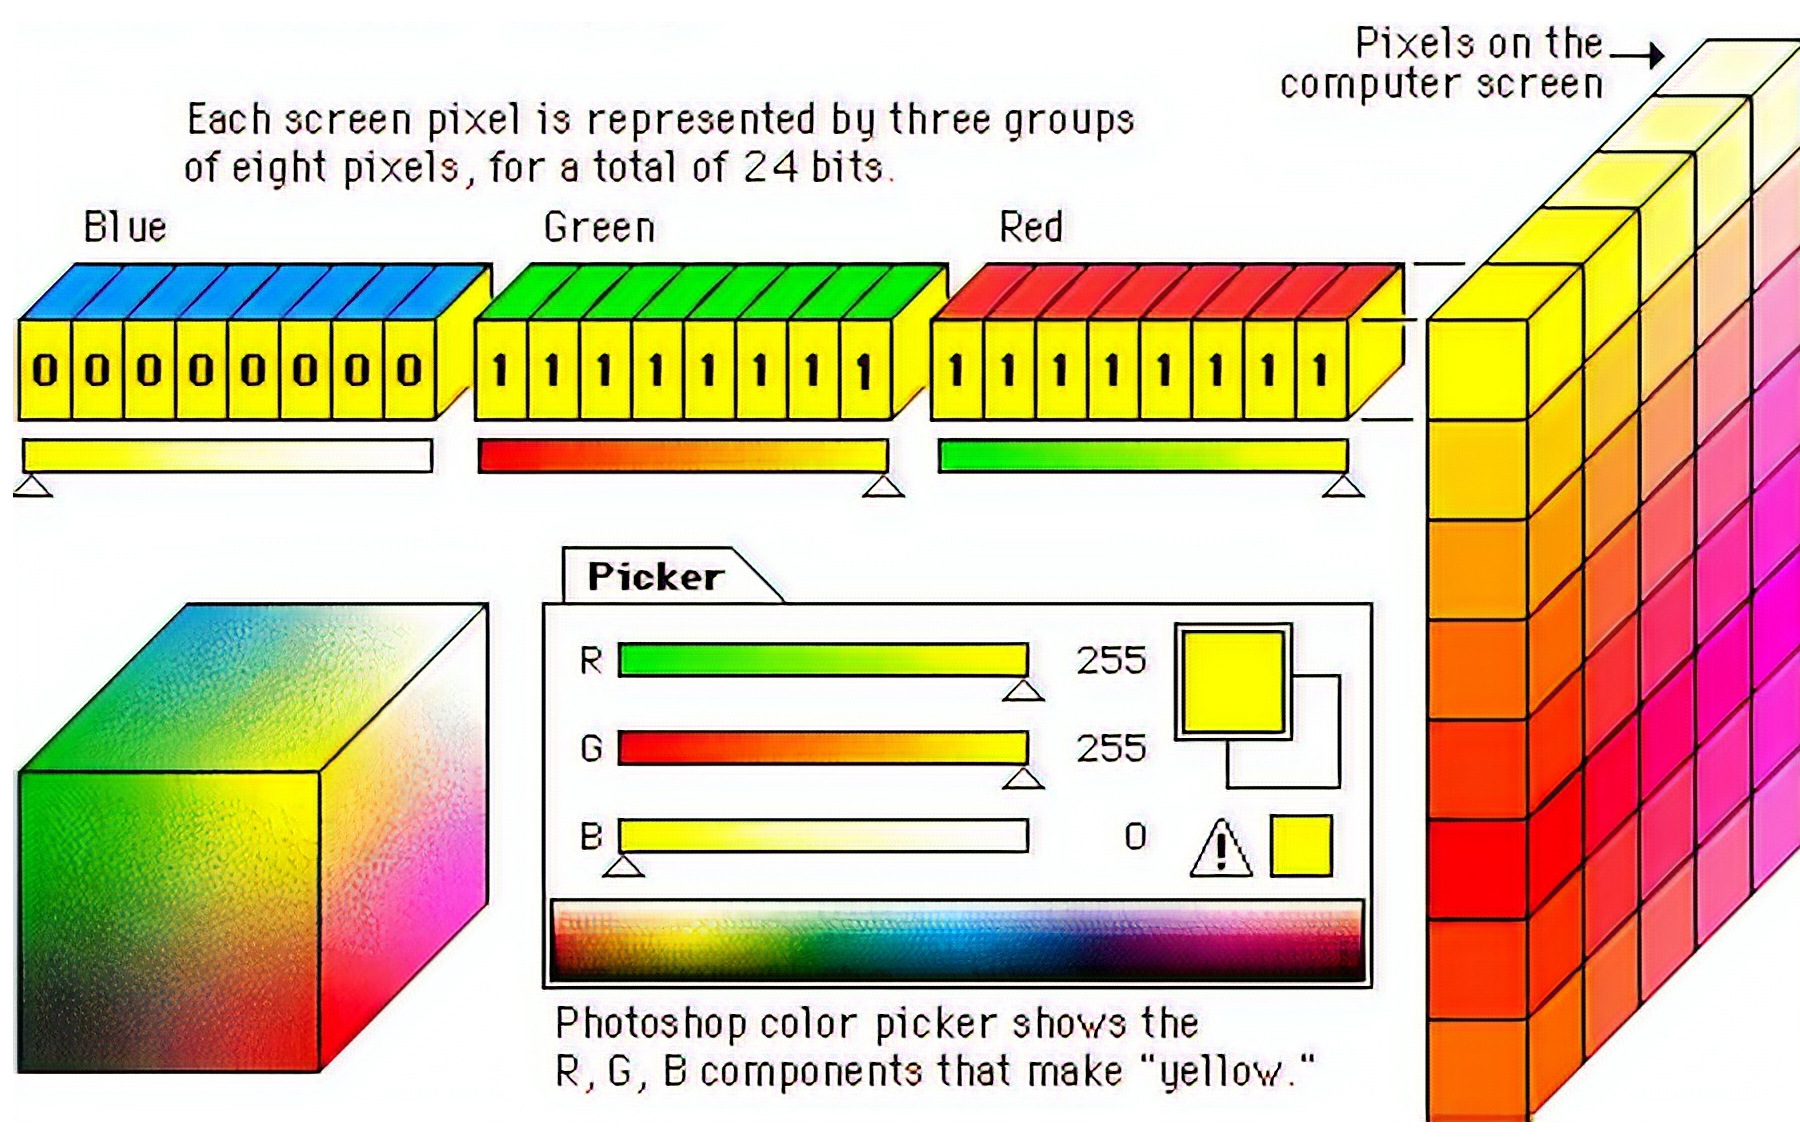
\includegraphics[width=0.8\linewidth]{figures/rgb}
	\caption{RGB color representation in 24-bit color display}
	\label{fig:rgb}
\end{figure}

In order to comprehend the broad range of computer vision, we shall understand the way computers "see" an image. Computers represent everything by binary numbers, meaning that it only consists of 0 and  1.  So images are no exception.   Machines interpret images as a series of pixels, each with their set of mathematical equivalent of color values as numbers.   In other words, an image is represented by a matrix, and each item in this matrix corresponds to a pixel; and the value of an item,  pixel in this context, represents the color values.  One can represent colors with numbers in many ways.  The most common method is to represent the level of red, green, and blue primary colors. By changing the respective amount of these colors, any desired color can be created. Each of these primary colors is represented by a 2-dimensional matrix of $height \times width$, in which each item represents the amount of the color in the corresponding pixel.\\

The range of colors is limited by the amount of bits assigned to each item.  If it is 8-bit, then we can have values ranging from 0 to 255 for each of the RGB primaries of the color, and in total, we can have 2563 = 16, 777, 216 different color combinations. Figure \ref{fig:rgb}\footnote{\url{https://cdn-images-1.medium.com/max/1600/0*I6XPXr9fzJ43L0ii.gif}} shows the way colors represented by machines.\\

As the involvement of machines in our daily lives escalated, human-computer interaction (HCI)  techniques became the main challenge for the computer vision community.   A typical example of these is controlling machines with commands performed by hands. As expected, image-based hand gesture recognition interfaces \cite{pavlovic_visual_1997} got popular really fast.  In the early years of computer vision, this had been done by creating models/templates of hands position and motion similar to many other applications of computer vision like object recognition.  Then it followed by extraction  of features using these templates.  And finally, an intelligent trajectory/motion recognition algorithm  used for classification \cite{jiang_dynamic_2013}. An example of this general form is shown in Figure \ref{fig:cv_gesture_workflow}.\\

\begin{figure}[h!]
	\centering
	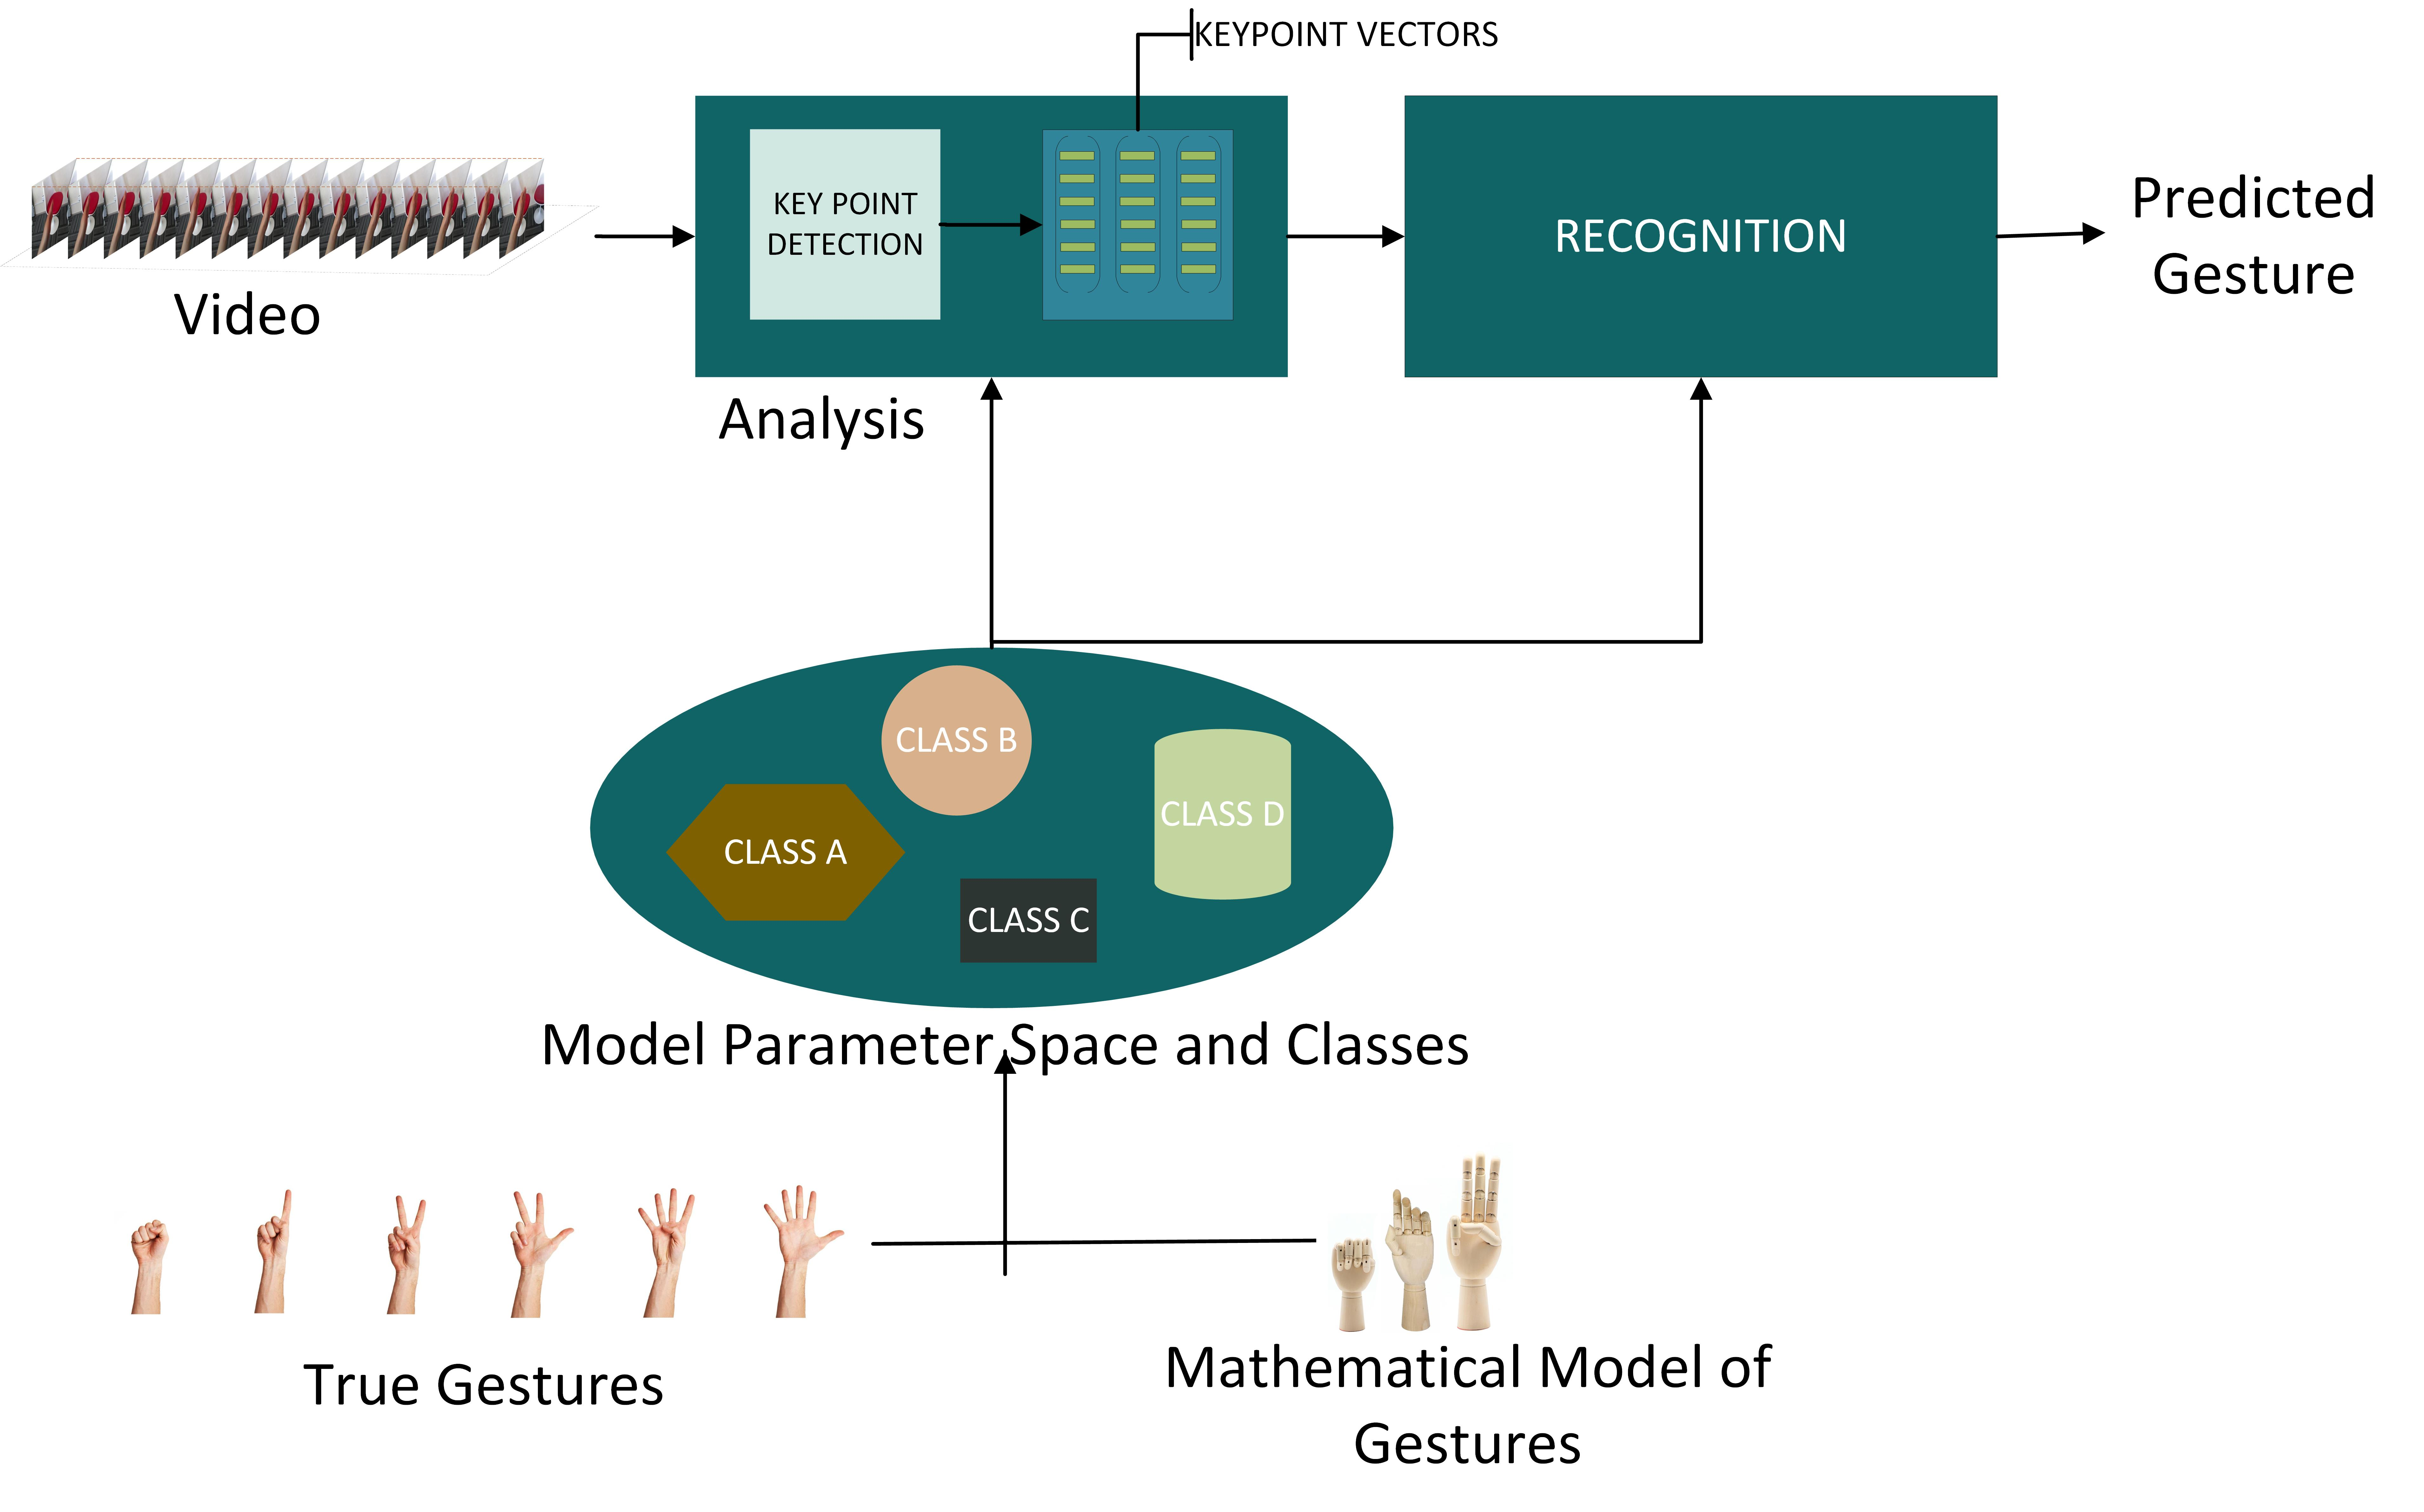
\includegraphics[width=0.8\linewidth]{figures/cv_gesture_workflow}
	\caption{A general framework of traditional gesture recognition system:  Each frame from the video stream is analyzed, and it is converted to a model space of the gestures.  After then  a recognition algorithm,  mostly k-means, predict  observed gesture.}
	\label{fig:cv_gesture_workflow}
\end{figure}

Although this approach showed some level of success, it is far from perfect.   For example, hand configuration is not always the same and has more than  26 degrees of freedom, and hand shape can change drastically depending on the view of the camera \cite{bergh_haarlet-based_2009}. One major drawback of this approach is that it is built upon many assumptions which have been taken for granted,  and either not general enough or too specific to the task.  Additionally,  computation requirements for most of these algorithms do not allow a robust real-time application system.  For a detailed background of computer vision researches on hand gesture recognition, please see Chapter  \ref{ch:relatedwork}.  These drawbacks brought up the question: "How  can we have a more reliable and robust algorithm for computer vision applications,  especially for the feature extraction phase?" With the availability of large datasets and the development of new computational devices like Graphical  Processing  Units  (GPUs),  it became possible that deep learning methods to show their true potential.   Consequently, conventional computer vision methods have been partly replaced by Deep Neural Networks in many application areas lately,  especially after the CNNs had proven their abilities in learning feature representations from images through the large publicly available datasets.\\

\section{Machine Learning} 
\label{sec:ML}

Machine learning is an application of Artificial  Intelligence  (AI)  which enables systems to automatically find patterns from the seen data without being preprogrammed.  Artificial neural networks (ANNs) or other methods of machine learning are mainly supervised technologies.  This means that, in addition to a large amount of input data, a substantial (best case equivalent) amount of corresponding labels is needed for this input data in order to sufficiently characterize the properties of the input data.  Those labels enable the machine learning method to find a meaningful connection between input data and its labels.  The general workflow of supervised machine learning task is illustrated in Figure \ref{fig:svml}: In (a) Training, the aim is to learn a classifier model function.In (b) Prediction,  the learned classifier model (output function of the machine learning algorithm)  can be used to classify new, previously unseen input data. The output/prediction of this classifier is a label for the new, previously unseen input. The portion of correctly classified input data gives the accuracy of the classifier model.\\
\begin{figure}[h]
	\centering
  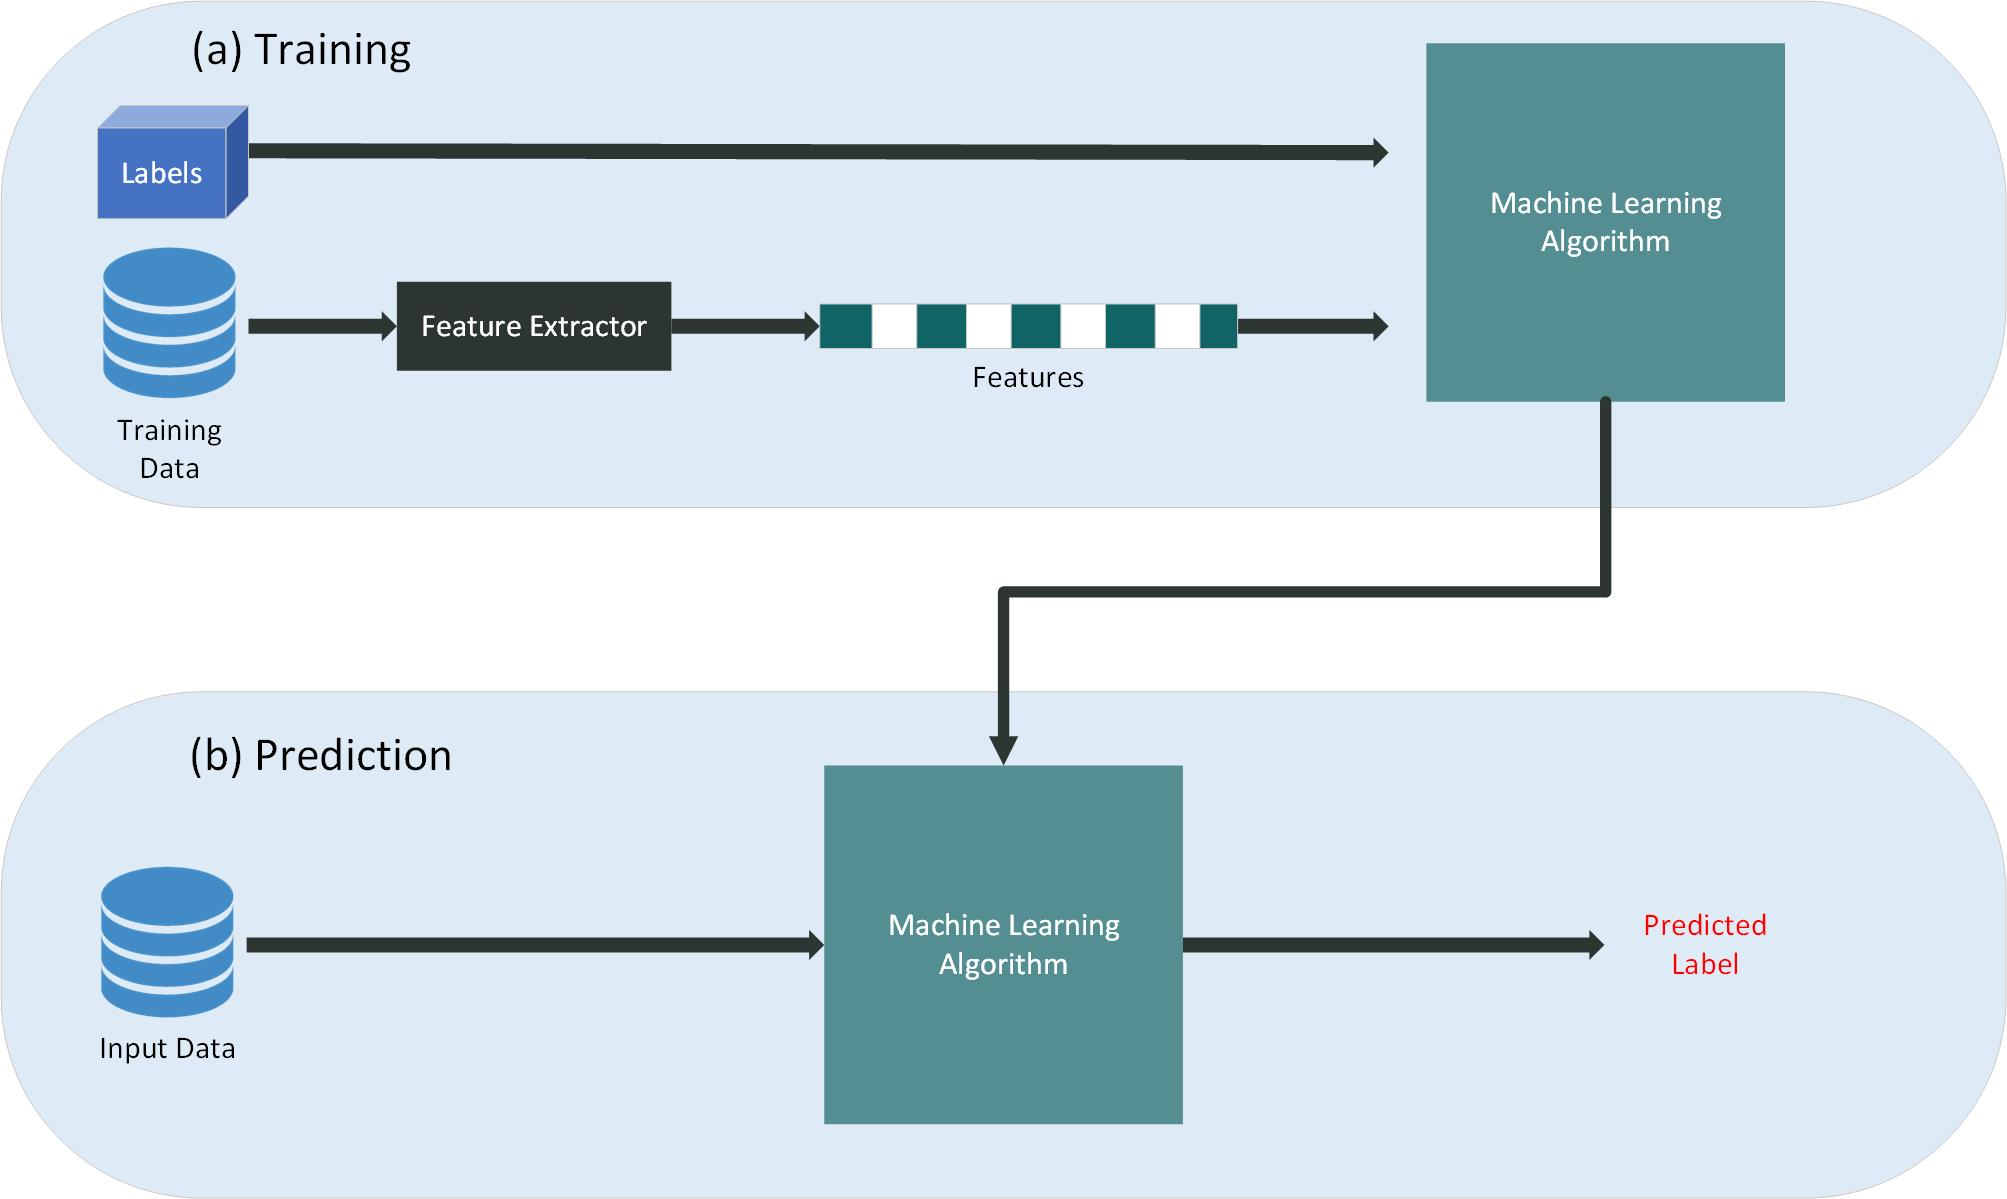
\includegraphics[width=\linewidth]{figures/ml_workflow}
  \caption{Supervised Machine Learning}
  \label{fig:svml}
\end{figure}

The concept of inferring a function from labeled training data,  which is described in the paragraph above and illustrated in Figure  \ref{fig:svml}, is called Supervised Machine Learning.  Methods of supervised machine learning include (among many others) regression, trees, random forests, nearest neighbor algorithms,  SVM (Support  Vector Machines), artificial neural networks, and many methods of deep learning, e.g. Convolutional  Neural Networks (CNNs), Long-Short-Term-Memory Networks (LSTMs),  or Neural Turing  Machines (NTM).\\

Apart from supervised machine learning, unsupervised machine learning (without labels) allows for finding patterns in the data,  also referred to as clustering.  Also, there is a third method; one can combine supervised and unsupervised learning methods if the small portion of the input data is labeled and the rest is unlabeled.  In a first step, patterns in the input data  are detected  in an unsupervised manner.  In a second step, the generated data pattern model is used as a pre-trained-model and labels, which are only available for a small portion of data set,  are used to add meaning to the previously structuring pre-trained model.   This method is called Semi-supervised learning,  see Figure  \ref{fig:ssml}. However,  for gesture recognition tasks,  - to the best of our knowledge- we almost always know the labels for the data in the training phase.   So, in this work,  we considered supervised learning.\\
\begin{figure}[h]
	\centering
  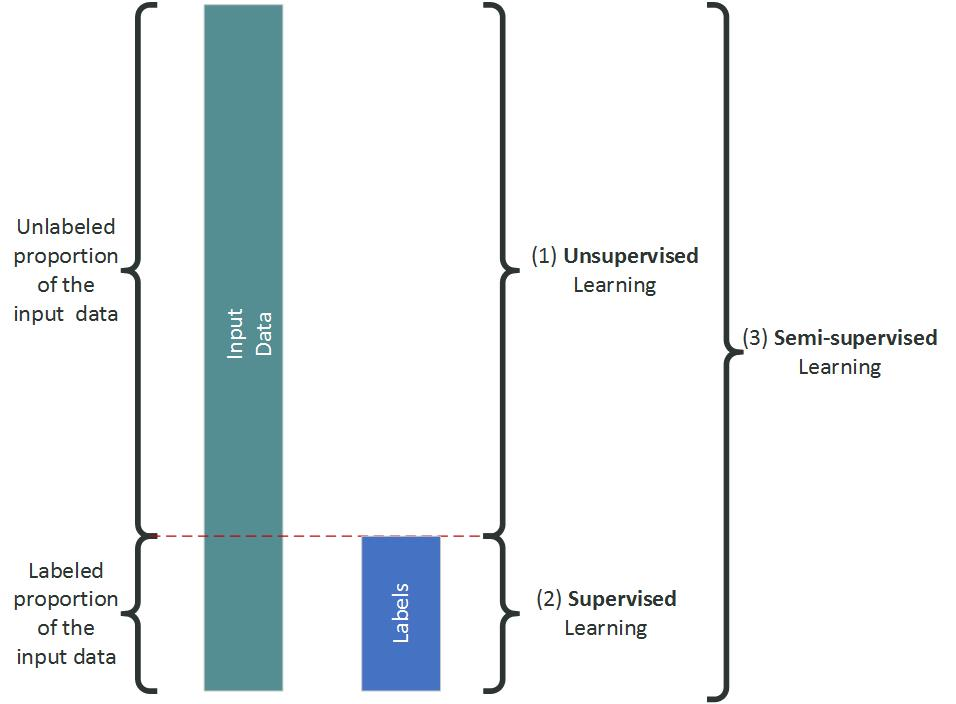
\includegraphics[height=0.6\linewidth]{figures/ml_learnings}
  \caption{Semi-Supervised Machine Learning for partly-labeled input data}
  \label{fig:ssml}
\end{figure}

Methods of Machine Learning are currently broadly used in a variety of sectors, also often referred to as methods of ”Artificial  Intelligence”  (AI).   Popular areas of application are, e.g., automatic image recognition,  automated driving or precise weather forecasts. Analysts evaluated AI’s potential as very high being a game changer for the technology of the 21st Century of humankind.  Naturally, computer vision has shared its part of the change, and in the last decade many computer vision tasks have been strengthened, evolved with the integration of more intelligent algorithms.  Convolutional  neural networks (CNNs) and its variations played an important part in this.  CNNs are being known for their ability in learning feature representations with a much lower number of parameters as opposed to the traditional fully-connected neural network.   As a consequence of this,  ”old-fashioned”  methods have been used in CV has been replaced by a CNN network.  In other words, the analysis and recognition parts in Figure \ref{fig:cv_gesture_workflow} are replaced by a machine learning algorithm, usually, a CNN network followed by a fully-connected network or LSTM network.\\


\subsection{Feed Forward Neural Networks}
\label{subsec:ffnn}
Artificial neural networks (ANNs) create the basis for many models in machine learning.  It is called ”neural”  because it is a brain-inspired system which is intended to imitate the way that we humans learn.  As a structure, it resembles a lot to the neural structure of human brains.  In some tasks which require mathematical calculations,  ANNs can find patterns which are far too complicated for a human programmer to extract and train the machine to recognize manually.  It consists of computing units called neuron,  and these neurons form a layer at which all neurons output together with a set of weights for one input. Each neuron in a layer is connected to all neurons in the consecutive layer through learned weights, refered as "fully-connected".  Neural networks consist of input,  output and (in most cases) hidden layers.  In Figure \ref{fig:ff}, the basic structure of a neuron and a simple fully-connected two layer networks are shown.\\
\begin{figure}[h]
	\centering
  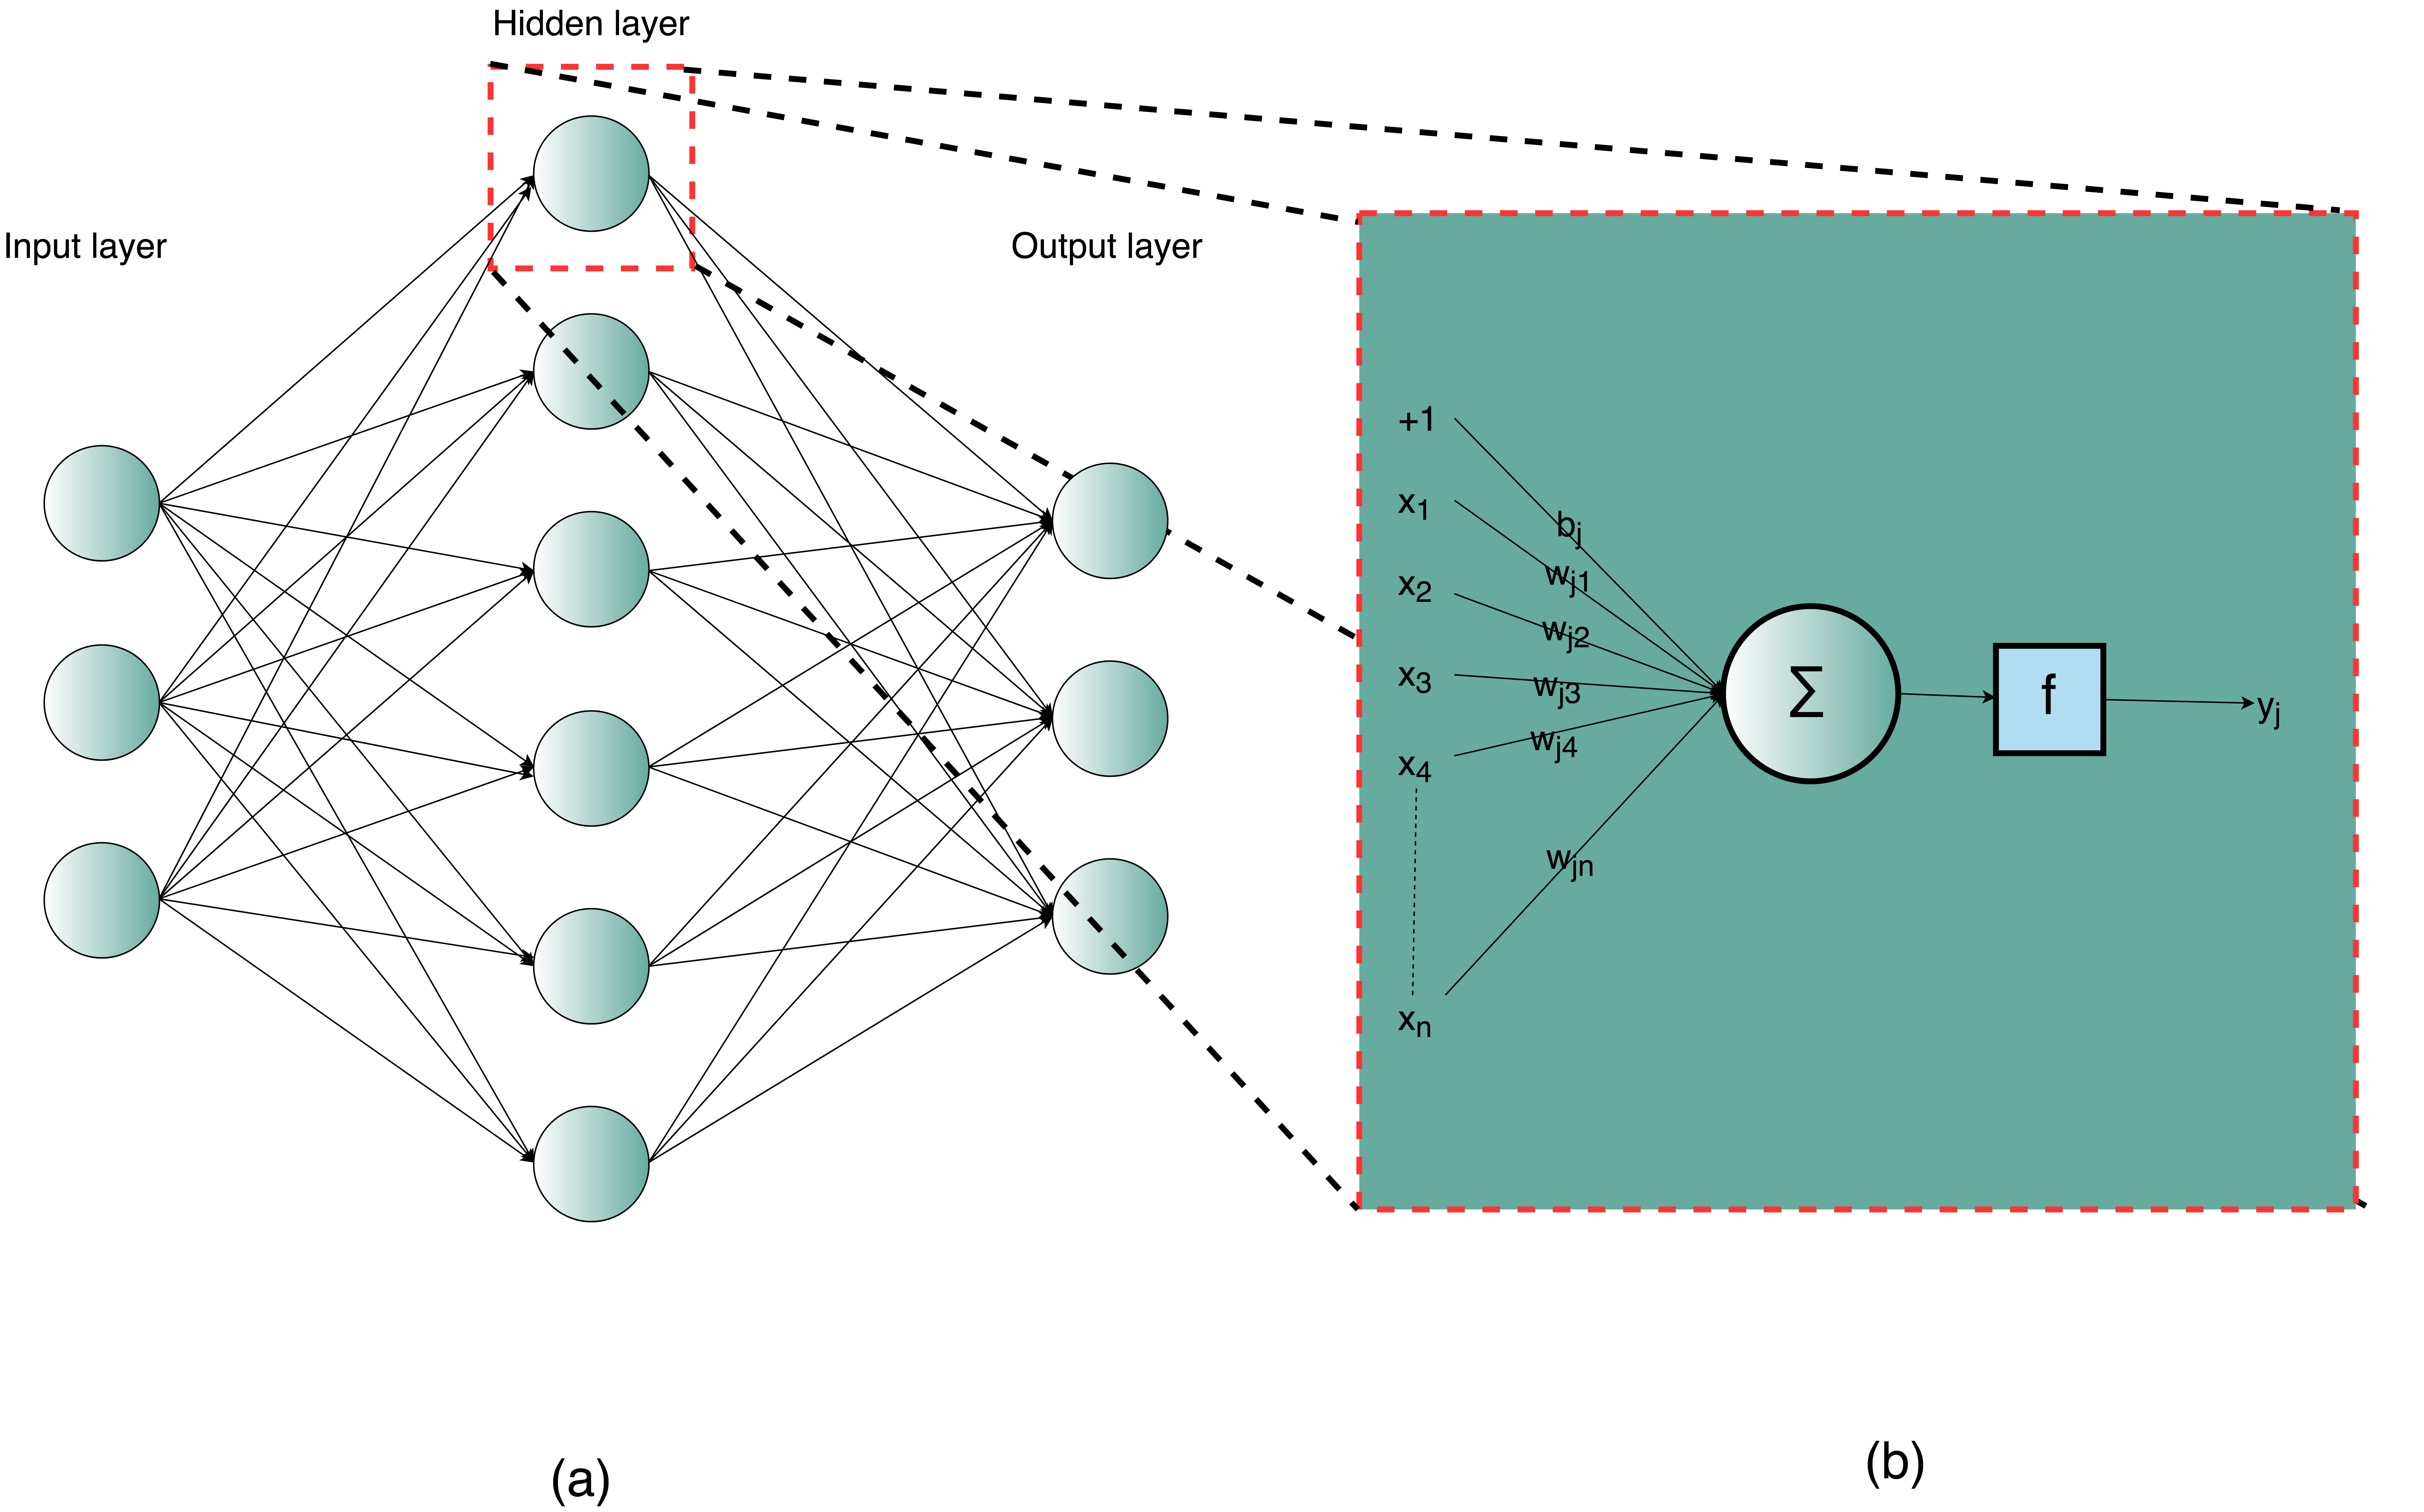
\includegraphics[width=\linewidth]{figures/ff_structure}
  \caption{An example ANNs structure: (a) A two-layer fully connected neural network with one hidden layer and output layer (b)  Structure of one neuron which is fed by n inputs and one bias term  (+1),  which are outputs of the previous layer, and an activation function f.}
  \label{fig:ff}
\end{figure}

Neural networks (perceptrons) roots back to the 1940s. They have become an essential method of artificial intelligence (AI)  in the last decades because of the discovery of the technique called \textbf{backpropagation}, which is derived from the chain-rule of mathematical derivation and allows neurons to adjust their weights according to the distance between the predicted outcome and the true outcome.\\

Another critical factor in the success of neural networks is the technological development in the last decade, which  make it possible to train deeper networks (\textbf{deep learning neural networks}). The most outstanding ability of the neural networks is to automatically learn to extract different features using backpropagation, which allow it to converge to the true label.  If the amount of the data is enough, then it can learn the feature representations without much of intervention by a practitioner. Besides that,  the deeper the neural network is, the better it learns distinctive features.\\ 

The most basic ANN model is the feedforward multilayer perceptron network (MLP) in which each neuron in one layer is connected to each neuron of the following layer \cite{goodfellow_deep_2016}, and these connections do not form a cycle.  This structure is also called a fully-connected neural network. Some other examples of feedforward networks are convolutional neural networks (CNNs) and  recurrent neural networks (RNNs) in which the information flows not only from input to output but also from output to input using feedback connections.  RNNs is a strong tool in complex tasks such as learning handwriting or language recognition in which there are temporal relations.  In this thesis, however, we will focus more on CNNs and their the ability in learning spatiotemporal relations, as we do not aim to desing a complex model that make use of, instead we aim for converting  any pretrained models into a real-time application with the use-case of vision-based gesture recognition.\\

\subsection{Convolutional Neural Networks (CNN)}
\label{subsec:cnn}
Convolutional  Neural Networks (CNNs) is biologically-inspired variants of Multilayer Perceptron (MLP).  It stems from a research in the 1960s on the brain of cats by Hubel and Wiesel \cite{hubel_receptive_1968}.  In order to understand convolutional neural networks we first need to understand how a human brain works.  For over 500 million years, the human brain and the visual system evolved to a system can differentiate and understand the 2-dimensional world and interpret it.\\

The process of learning starts during the very earliest year of our life.  For example, if we want a child to understand the difference between a dog and a cat,  he/she should have seen at least some cats and dogs.  Similarly, an algorithm needs to be fed by an enormous number of pictures of cats and dogs before it can make correct predictions when a new image is shown. \\

On the other hand,  we also need to understand that computers  ”see” in a different way than we do. As it is shown in Figure \ref{fig:rgb}, computers represent everything by numbers,  specifically binary numbers,  as it is the case for the images as well. Every image is a 2-dimensional array of pixels. Fortunately, we can still train machines even though their perception of images is different from humans.  In Figure \ref{fig:image2d} \footnote{\url{http://cs231n.github.io/classification/}}, an example image of a cat is shown, and on the right side of it, we can observe what computer  ”sees”, which is nothing but a collection of numbers.\\
\begin{figure}[h!]
	\centering
  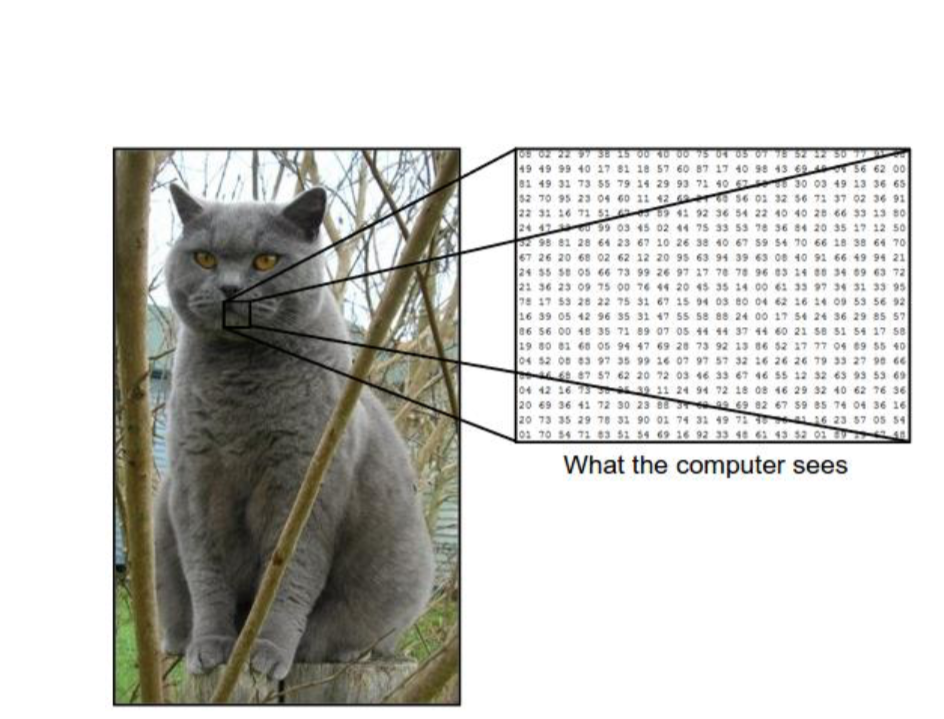
\includegraphics[width=0.7\linewidth]{figures/howcomputersees.png} 
  \caption{Representation of a cat image as a two-dimensional array of numbers.}
  \label{fig:image2d}
\end{figure}



In the late 60s, Hubel et al. discovered that the visual cortex consists of a complex arrangement of cells in the brain of cats and monkeys.  Also, these cells individually respond to specific regions.  In other words, They are more sensitive to smaller regions of the visual field - it is also called the receptive field.\\

Additionally,  in this paper two basic cell types, which act differently depending on the trigger, are described:  1) \textbf{Simple cells} activate when edge-like patterns or basic shapes like a line in their receptive field. 2) \textbf{Complex cells} are invariant to the position of a figure, so they activate whenever a known pattern is detected regardless of its position in the visual field.\\

The visual cortex of mammals being the most impressive image processing system has always been an inspiration in the computer vision community.  A few examples of many models inspired by this concept are (1) \textbf{Neocogrition} \cite{fukushima_neocognitron_2007}, in which a multi-layered artificial neural network proposed based on the concept of the Simple and Complex cells and later served as the inspiration  for CNN, and (2) \textbf{LeNet-5} \cite{lecun_gradient-based_1998} which is considered as the first Convolutional  Neural Network, and it was able to classify digits from handwritten  numbers.  In recent years, Convolutional  Neural Networks (CNN) has found its position as the most successful method to learn and  recognize patterns from images.  In the rest of this section, we introduce the basic architecture of CNNs and one of its variant, called ResNet \cite{he_deep_2015}, because we mainly focused on these two methods in this thesis.\\

The name ”convolution”  stem from convolution operation ($\circledast$) in mathematics. This is because in CNN we have filters similar to Simple cells convolved over the output array of the previous layer.   This operation allows us to find any patterns regardless of the position of it in the image, which means the convolution operation mimics the ability of Complex cells.\\

It is important to note that  there are three primary motivations for CNNs: \textbf{Sparse interaction}, \textbf{Parameter sharing}, and \textbf{Equivalence}.\\\\\\

\textbf{(a) Sparse interaction :}\\
\begin{figure}[b!]
	\centering
  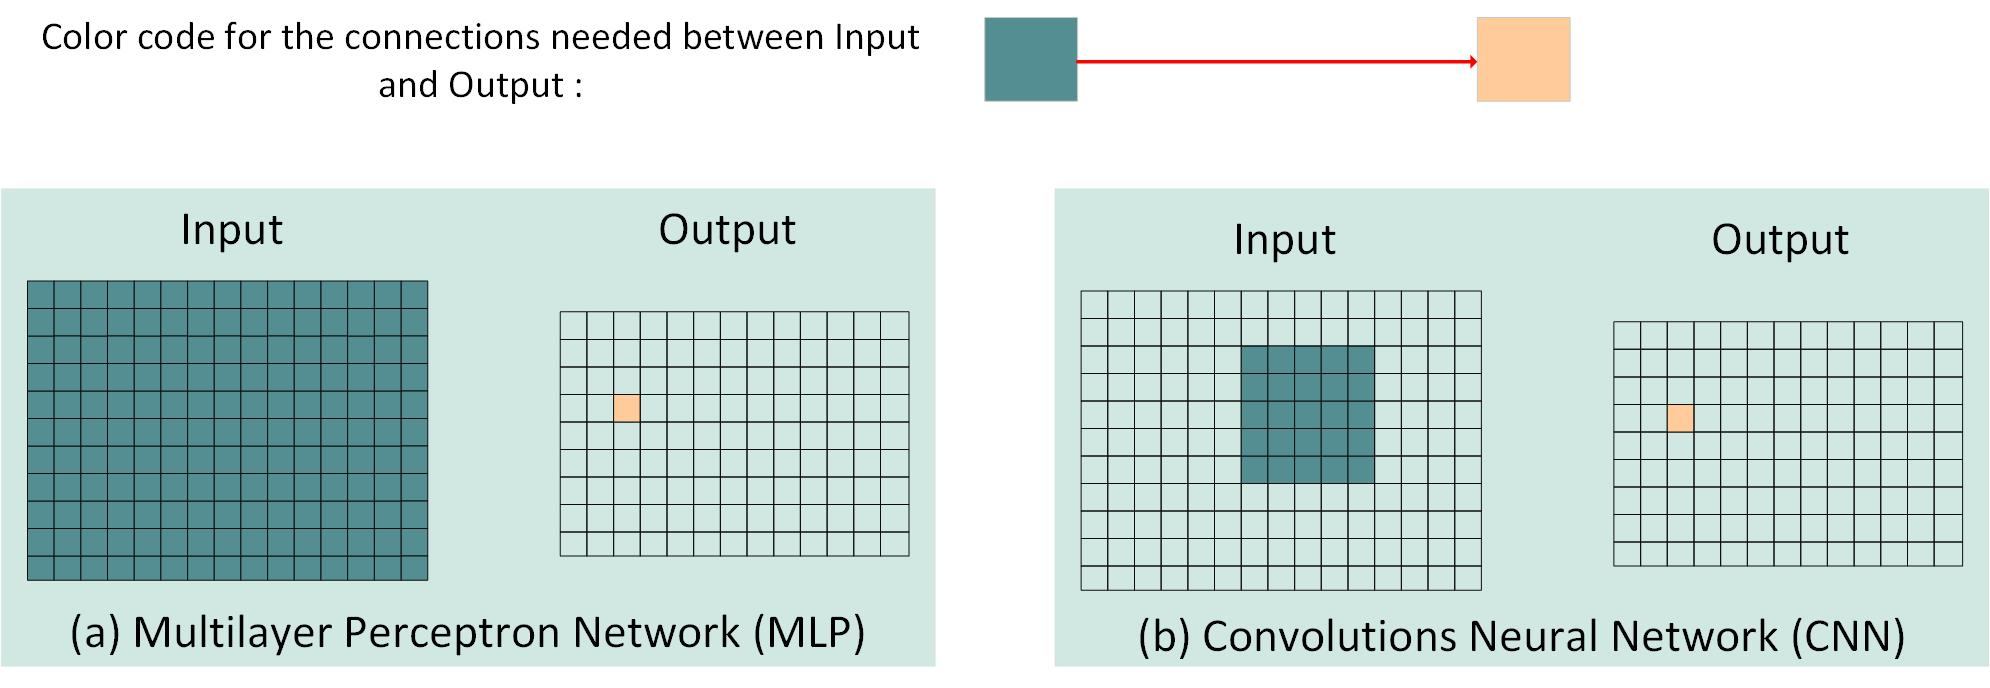
\includegraphics[width=\linewidth]{figures/mlpvscnn} 
  \caption{Comparison of MLP and CNNs in terms of number of connections needed between two layers.}
  \label{fig:mlpvscnn}
\end{figure}

Any process on images requires a lot of computational power because images naturally have bigger size compared to time-series and many other data types.  The way CNN handle this is called sparse interaction.  It is also called sparse weights since it aims to make kernels (also called as filters) smaller input.  By this, the model can have fewer parameters compared to fully-connected networks, and consequently, it reduces memory consumption and CPU operations,  and training will take much less time than training and MLP model.\\

For example, we want to compare the number of parameters to learn for MLP and CNN in case we have an input image of total m pixels (neurons)  and output of n pixels (neurons) in the following layer.  In MLP,  we need to have all m neurons to be connected to each output neuron, so as a result, we will have $m \times n$ parameters (weights).  However, for CNN, we need pixels in the ”receptive field” of size k to be connected to output pixels. In this case, we will have $k \times n$ connections, see Figure \ref{fig:mlpvscnn}. Usually $k \\ll m$, and consequently we will have much fewer operations and parameters to learn by using the concept of receptive field in the Visual cortex. \\

\textbf{(b) Parameter Sharing :}\\

As it is shown in Figure \ref{fig:prsharing}, in CNN the model only learns a set of parameters instead of learning parameters (weights)  for each of the connection like in MLP. It is clear that the number of weights, shown by annotation of W, is decreased by a factor of 4 even for an input layer of 4 neurons to a layer of 5 neurons.  Also, it is worth to note that, number of neurons is in 3 digits for image processing tasks, so parameter sharing makes a significant decrease in memory consumption. \\
\begin{figure}[h!]
	\centering
  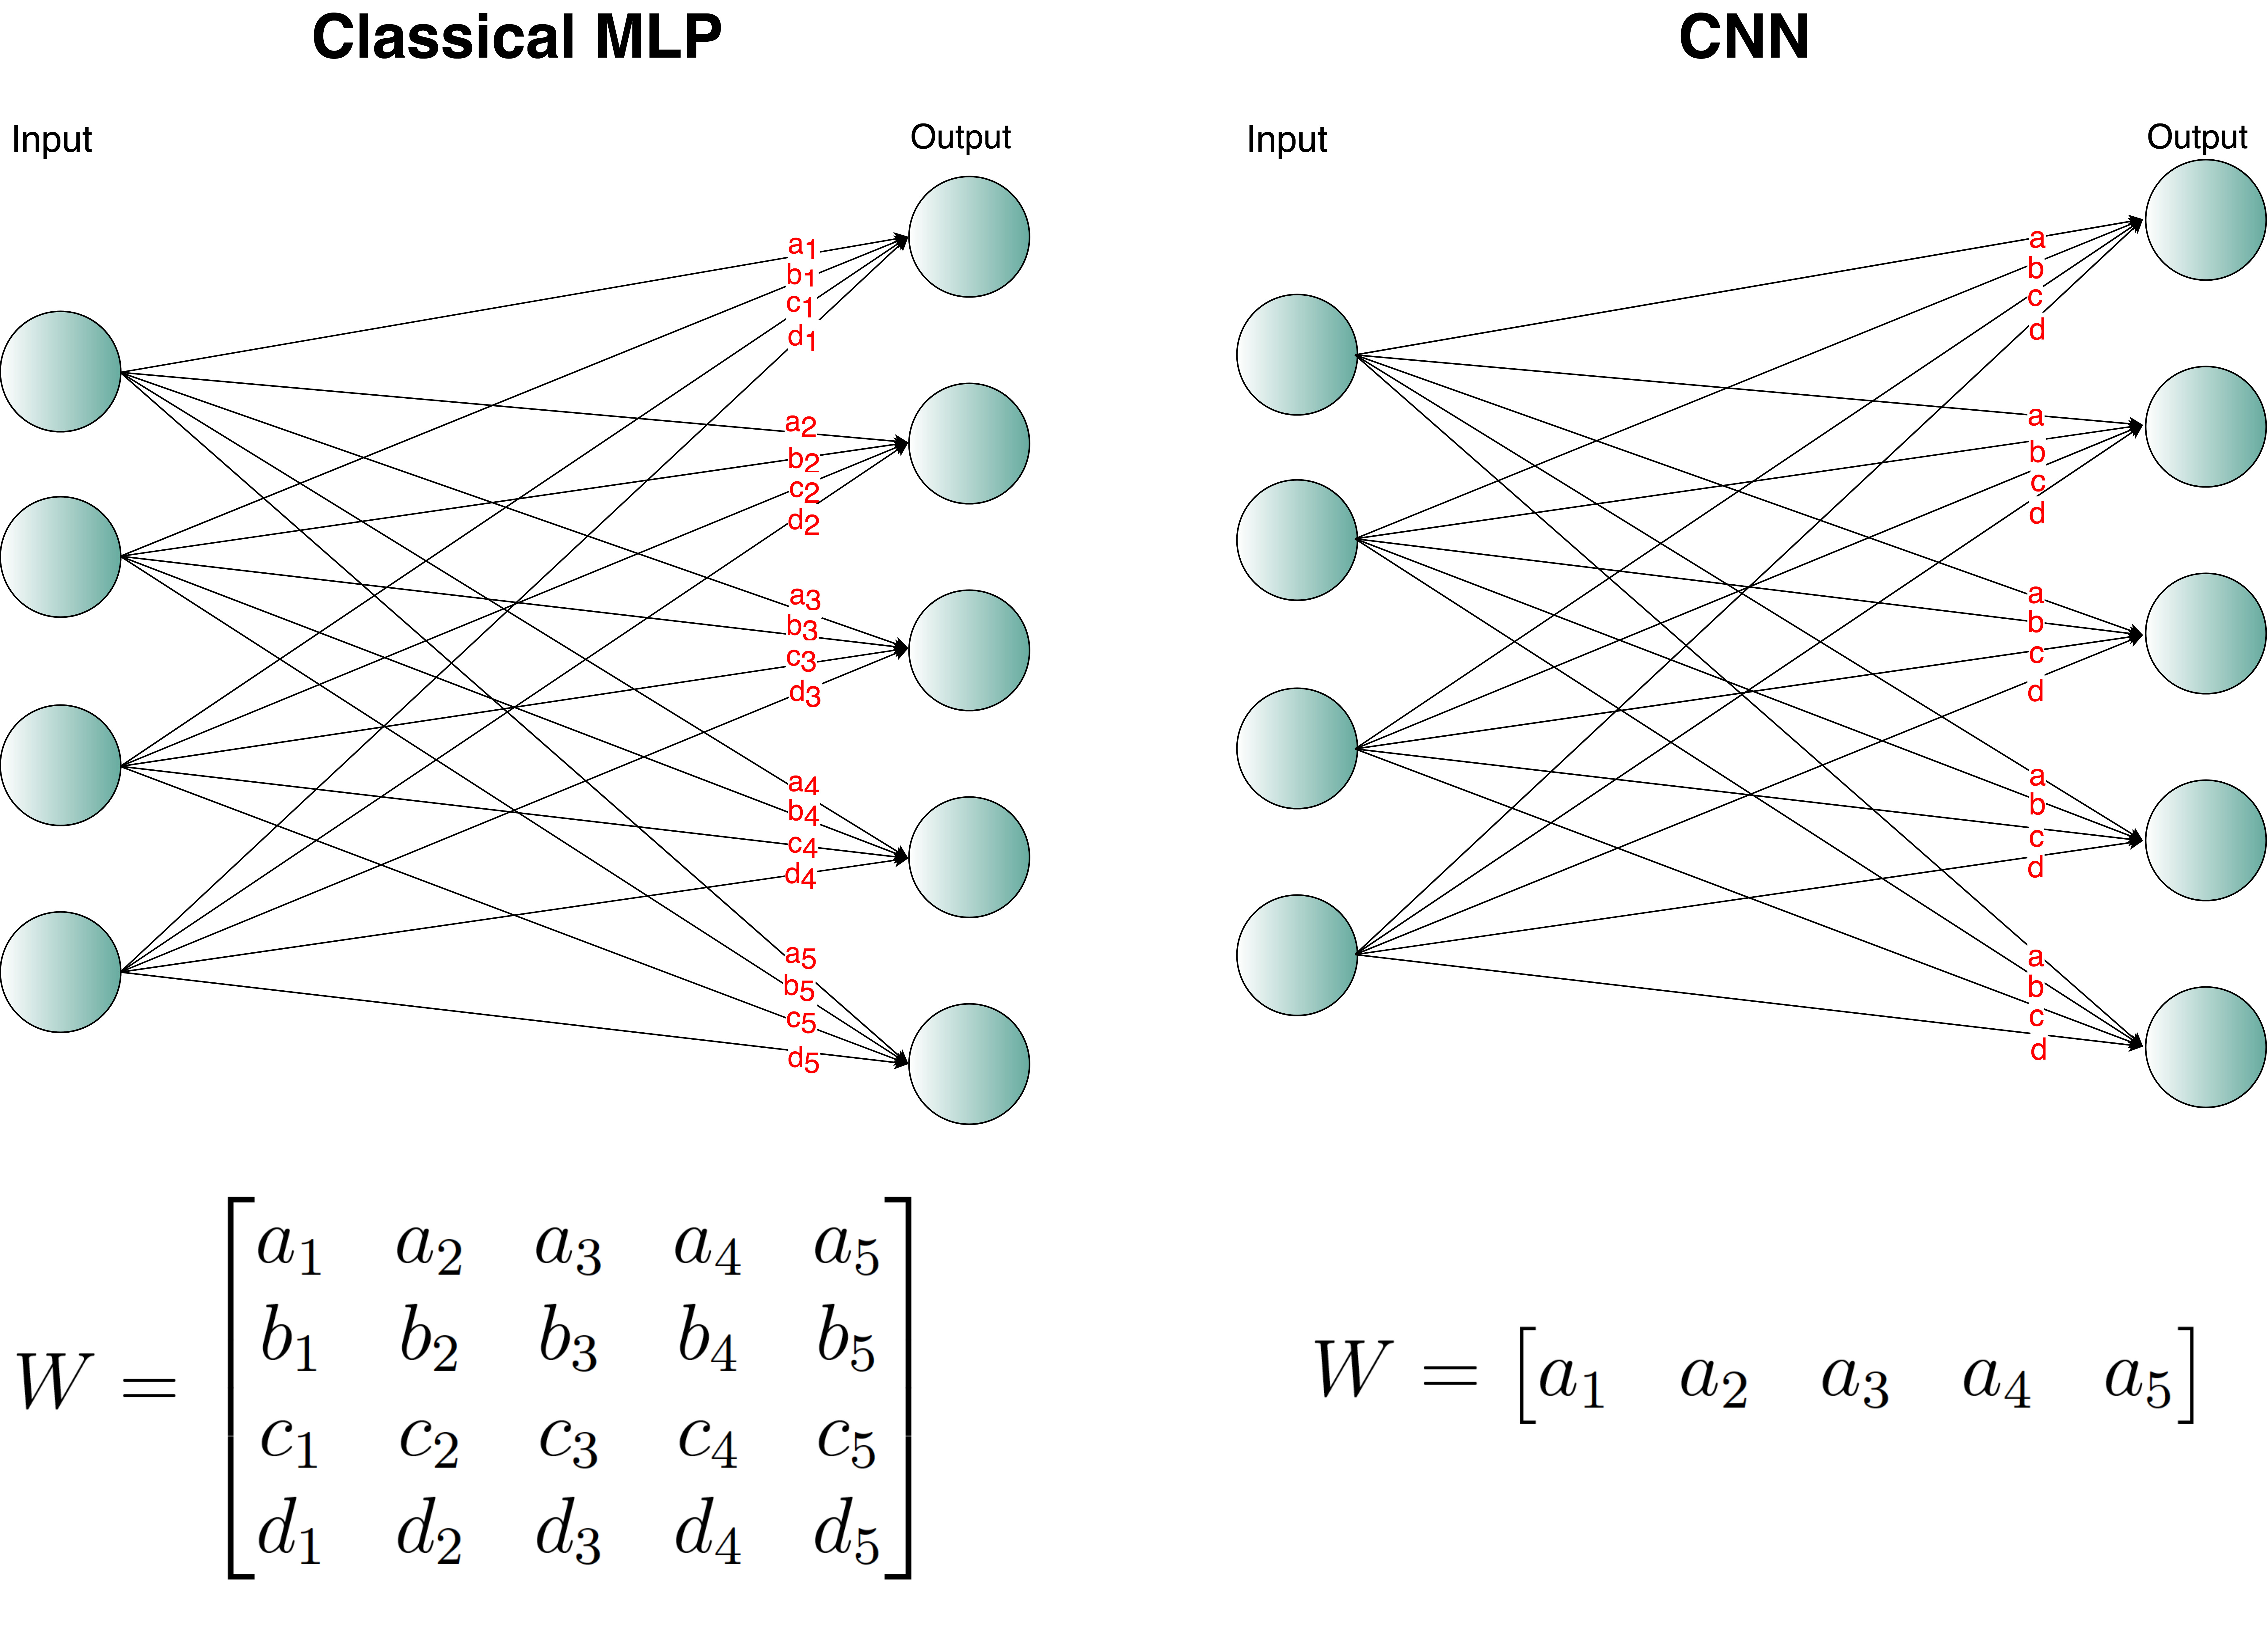
\includegraphics[width=0.8\linewidth, height=0.5\linewidth ]{figures/parameter_sharing} 
  \caption{Parameters needed in classical fully-connected network (on the left) and convolutional neural network (on the right).}
  \label{fig:prsharing}
\end{figure}
\clearpage
\textbf{(c) Equivalence :}\\

if  $f(g(x)) = g(f(x))$, then $f(x)$ is equivalent to g.  For example, CNN is equivalent to translation in images, meaning that any change in the position of an object in the image is observed in the output in the same manner.  This property is different from invariance.
\begin{itemize}
\item \textbf{Invariance} means the  internal  representation of an object  does not  change when the properties  of that  object change, $f(g(x)) = f(x)$,
\item \textbf{Equivalence} means  the  internal  representation captures  the  properties  of the object, $f(g(x)) = g(f(x))$. 
\end{itemize}

In CV tasks, there are three main operations where algorithms aim to be invariant to translation, scaling, and rotation.  CNN only brings equivalence to the solution. However, with the help of max pooling operation after convolution operation we can solve the problem of invariance.  For the sake of simplicity, we investigate 2D convolutional neural networks (CNNs) architecture in the rest of this section. \\
\begin{figure}[t!]
	\centering
  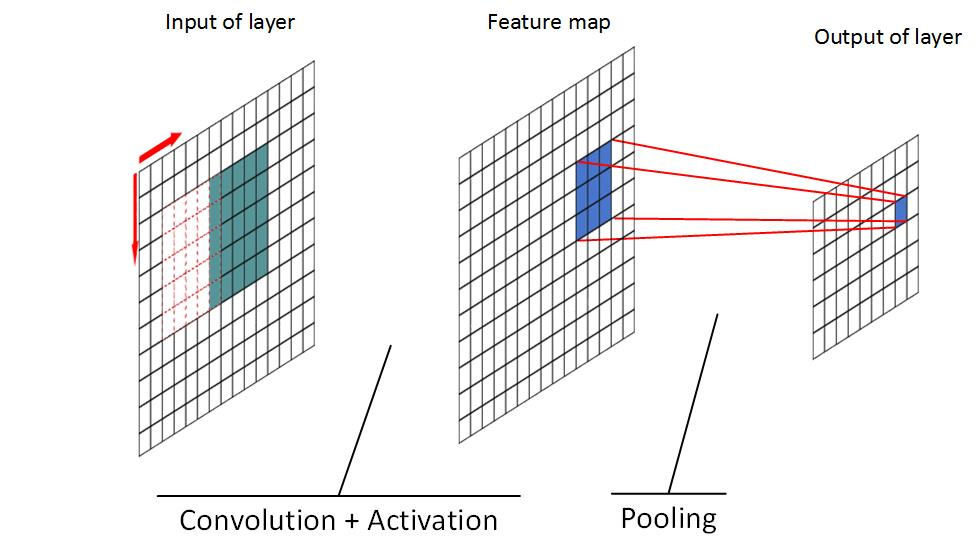
\includegraphics[width=0.8\linewidth]{figures/cnn_stages}  
  \caption{A basic convolutional layer, which consists of a convolution operation followed by an activation, and at the end pooling (a popular example is  max-pooling) operation is applied. It can be observed that the size of input image is shallowed.}
  \label{fig:cnnstages}
\end{figure}

Convolutional neural networks is essentially a variant of fully connected Multilayer perceptron network (MLP). In the sense of the layer structure and operations between input and neuron weights except for convolution, and pooling operations.  In both of networks, data flow forward, unlike recurrent neural networks (RNN), through weights, and the core functionality is done by a simple dot product between weights and input. Besides, in both types of these networks the resulting outcome of dot product pass through an activation function as shown in Equation  \ref{eq:dot}, such as ReLu, sigmoid, or tanh.  In Figure \ref{fig:mlpvscnn}, one significant difference between CNNs and MLP is shown, which is that in CNN the connections between input and output is local but in MLP it is fully connected regardless of the region of the input data \cite{lecun_gradient-based_1998}.\\

\begin{equation}
\label{eq:dot}
\begin{aligned}
  a_{xy} =& \sum\limits_{i}\sum\limits_{j}(w_{ij}\cdot v_{x+i,y+j} + b),\\
  z_{xy} =& f(a_{xy}),
\end{aligned}
\end{equation}

in which $v_{x+i,y+j}$ is input at the position $(x+i,y+j)$, b is the bias term, $w_{ij}$ weight of the kernel at position $(i,j)$, $a_{x,y}$ is the output of the summation at $(x,y)$, $f(..)$ is an \textit{activation function}, and lastly $z_{xy}$ is the output at position $(x,y)$, $z$ as a whole is also called \textit{feature map}. \\

One layer of CNN mainly consists of 3 stages:   convolution,  activation, and pooling stages see Figure \ref{fig:cnnstages}. Convolution layer, as the name implies, convolve a kernel (filter) of specified size than input over the input image. Later it is fed into an activation function, Usually Rectified Linear Unit (ReLu) activation function shown in Figure \ref{fig:activations}\footnote{\url{https://cdn-images-1.medium.com/max/1200/1*ZafDv3VUm60Eh10OeJu1vw.png}}. After that, a pooling operation is performed over a specified size.  This operation is quite similar to convolution operations except we do not have any parameters to learn in this stage unlike in convolution stage.\\

\begin{figure}[h!]
	\centering
  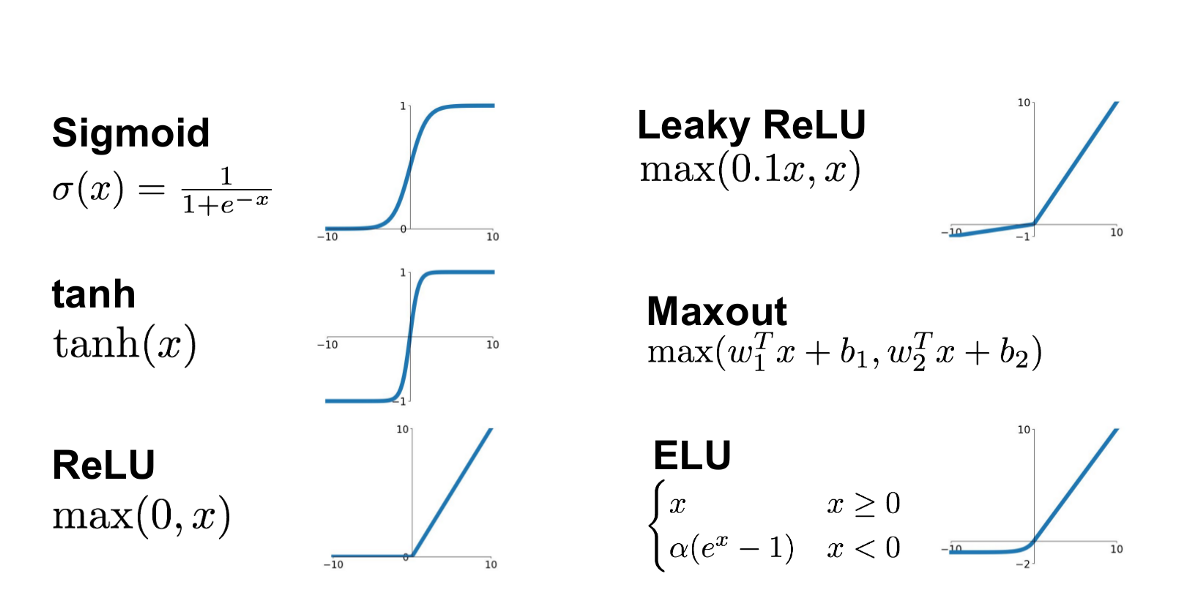
\includegraphics[width=0.8\linewidth]{figures/activations.png} 
  \caption{Some examples of activations functions.}
  \label{fig:activations}
\end{figure}

As I mentioned before, there are three transformations in images need to be tackled in CV tasks.  These are scaling, rotation and translation.  The convolution and pooling operations handle translation since it mimics the "receptive field" concept\footnote{\url{http://cs231n.github.io/}} by creating local connections between input and feature map.  Scaling problem,  on the other hand, is been solved pooling operation,  which maps a 2-dimensional subregion of feature map to one value.  Two most popular pooling strategies have proved to work well are \textit{Max Polling} and \textit{Average Pooling}.  Lastly, the rotation could be only achieved by either increasing samples from different angles in the training data or applying some augmentation methods.  It is important to note that  , augmentation methods  can work for scaling and translation as well and improve the performance a lot.\\

\begin{figure}[t!]
	\centering
  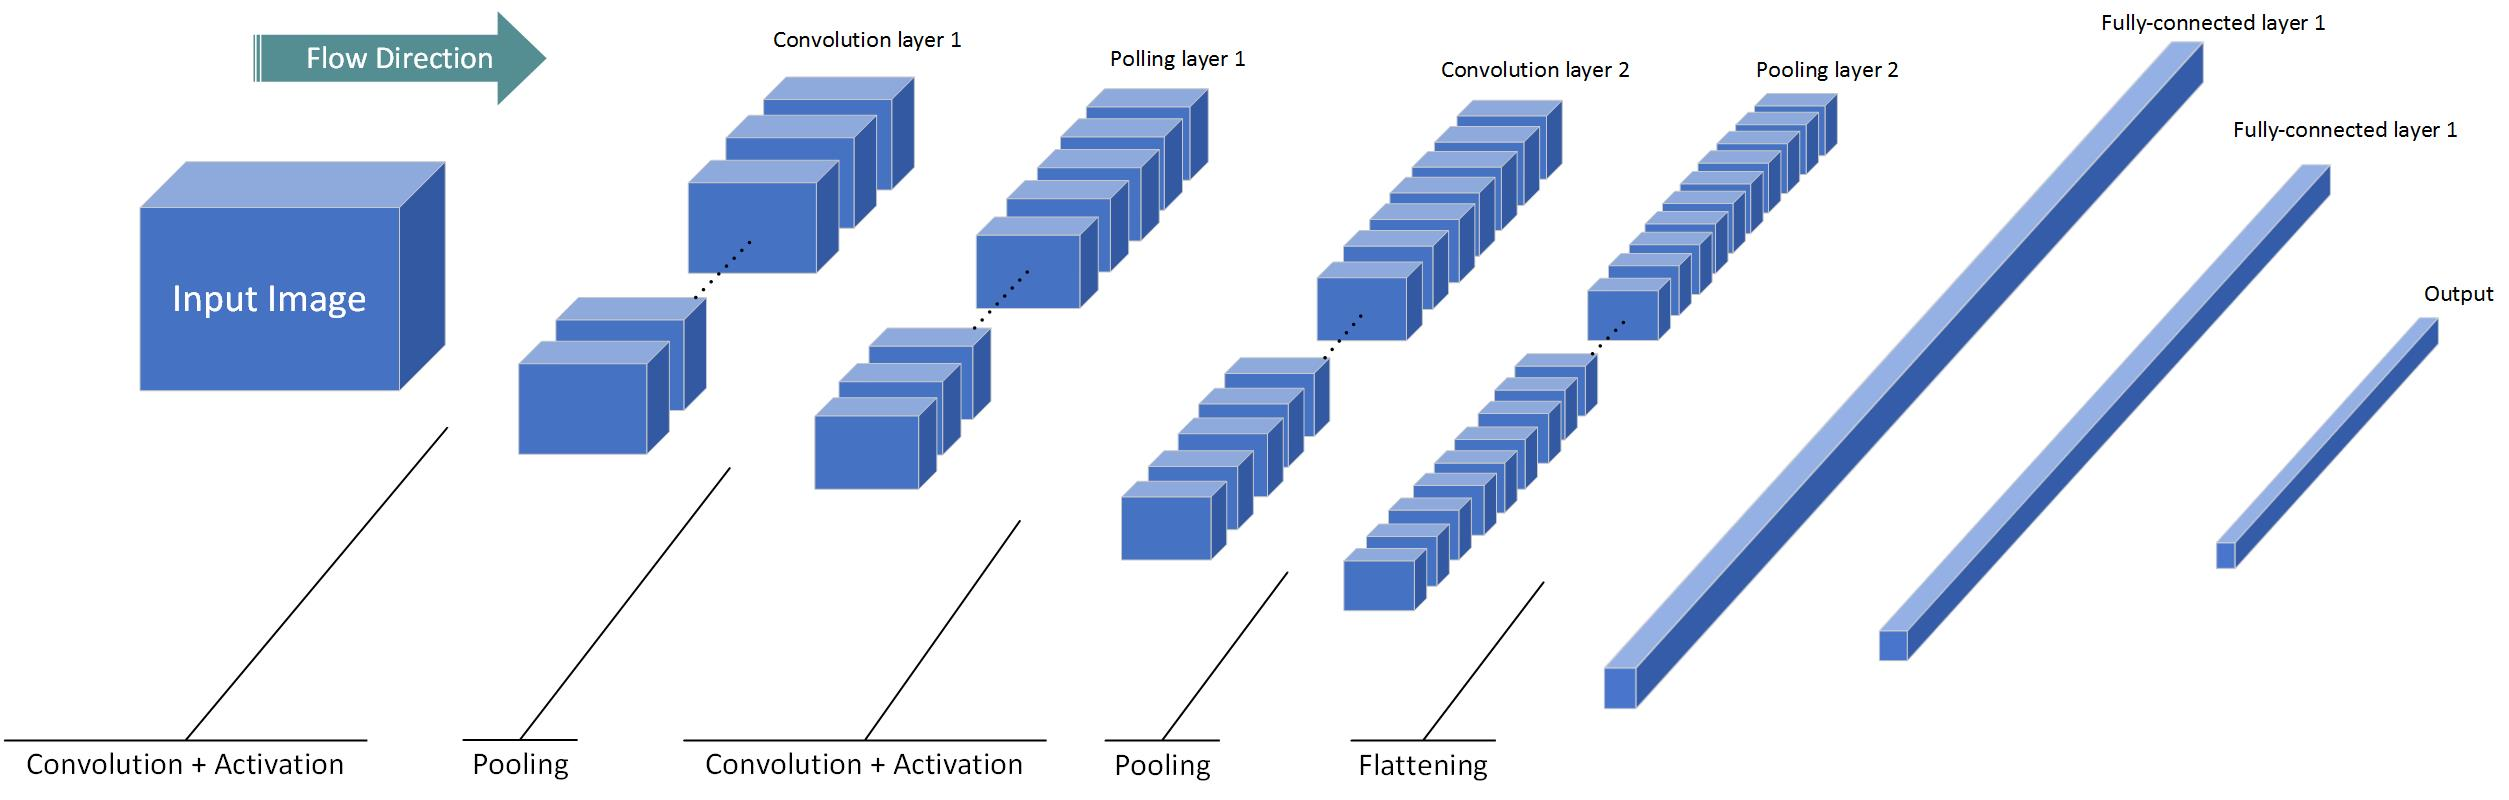
\includegraphics[width=\linewidth]{figures/cnn_whole} 
  \caption{An example of convolutional neural network model on images. It consists of two concolutional layer, and 3 fully connected layer on top of it. The last layer of the model should have a size equal to the number of classes.}
  \label{fig:cnn_whole}
\end{figure}

The general structure of a Convolutional neural network (CNN) with two convolution layers, each followed by a pooling layer, and two fully-connected layers are shown in Figure \ref{fig:cnn_whole}.  As I mentioned before, CNN is a powerful feature  extractor, and the responsible layers for feature extraction are convolution layers. In the end, we assume that the right features are created and on top of it any machine learning method can be applied. Although this is the case, most of the times this machine learning method is a fully-connected multilayer perceptron network (MLP)  as it is shown in Figure \ref{fig:cnn_whole} because we can train our network  on the fly with this structure.  Imagine if we want to use a Support  Vector  Machine (SVM), then we cannot train the whole network as a whole, instead we need first to train a CNN + MLP network and then use only convolution layers’ output to train an SVM.\\


Besides this structure, there are many other CNN-inspired methods developed.  One of the most powerful one recently developed by K. He and X. Zhang is ResNet \cite{he_deep_2015}. ResNet stands for Residual Network, and the idea of this paper is bypassing the input to the output of two consequtive convolution layer.  By doing so, it allows back-propagation from output to the input more efficient and solves the vanishing gradient problem, which is a phenomena happens when gradient converges to zero as the number of layers increases in the network.\\

In Figure \ref{fig:blocks}, basic residual blocks of ResNet (at the left side) and ResNext (at the right side) are shown. A ResNet block has two convolutional layers followed by a batch normalization and a ReLU activation.   Like all residuals block, there is a connection between input and output between second batch normalization and ReLU operation.    This structure is first introduced in \cite{he_deep_2015}, and it allows for training networks with more than 100 layers.    This revolutionized Computer   Vision/  Deep Learning community as training deep networks is one of the main challenges. In \cite{he_identity_2016}, researchers achieved to train even 1001-layered ResNet.   Because of its appealing results in many tasks, ResNet quickly became popular in the research community.  There are many variants of ResNet developed in  3 years by changing the structure of the residual block.  In ResNext, the residual block has many parallel convolutions and one bypass connection from the input to the output.  One of the most successful ones is called ResNext whose basic block is shown at the right side of Figure \ref{fig:blocks}, and in this thesis, we will use ResNext-101 \cite{xie_aggregated_2016} and C3D \cite{tran_learning_2014}, which is also a well-known 3D CNN architecture,  as our classifiers. ResNet-10, on the other hand,  will be used for the detection of gestures as it has a relatively much smaller structure as detection task does not require a complex and heavy model. \\



% Related work
\chapter{Related Work}
\label{ch:relatedwork}

In recent years, with the development of powerful graphical processing units  (GPU), Deep neural networks (DNNs) has got deeper and deeper.  Relatedly, they grow even stronger by performing much better against conventional computer vision methods in many challenging tasks like gesture recognition.  The types of DNNs have also been increased exponentially  in the last decade.  Some of the most popular ones are Convolutional neural networks (CNNs), Recurrent neural networks (RNNs), and Generative adversarial networks (GANs).  Especially CNNs and its variants are very popular in computer vision community as a result of the fact that  CNN proves to work better than conventional computer vision methods in which machine learning methods build upon hand-crafted features when the dataset is large enough  \cite{krizhevsky2012imagenet}.\\

On the other hand, the number of available datasets in many areas increased drastically as a result of this success story.   In this \href{https://en.wikipedia.org/wiki/List_of_datasets_for_machine_learning_research}{link},  a list of popular open-source datasets can be found.   There are also many public datasets for action/gesture recognition tasks.   Some of these  datasets  are  Human  Motion  Data  Base (HMDB51)  \cite{kuehne_hmdb51:_2011}, Kinetics \cite{kay_kinetics_2017}, UCF 101 \cite{soomro_ucf101:_2012}, ActivityNet  \cite{heilbron_activitynet:_2015}, Jester  \cite{twentybn_20bn-jester_nodate}, Something- Something \cite{goyal_something_2017}, EgoGesture \cite{zhang_egogesture:_2018} and many more. Researchers’ focus has been mainly on how to achieve the best accuracy by trying different models like in 2D tasks.  However, there is another question need to be answered here, and it is how to convert these models into a system works in real-time scenarios with the same accuracy as in offline classification.\\

With the availability of large datasets  (especially ImageNet),  CNNs has been used even more on 2D images where it can capture spatial information better than it ever had.  This changed the direction of researches to a whole new level.  New models were being trained first on ImageNet and then tuned on the dataset of interest.  Some example of this kind of applications can be face recognition, handwriting and character recognition,  and person recognition. The success of CNNs in object detection and classification tasks \cite{krizhevsky2012imagenet, zhou2014learning, Girshick2014rich} has created a growing trend to apply them also in other areas of computer vision.  Of course, the video action and activity recognition was one of the first application areas to apply  CNNs and achieve state-of-the-art performance \cite{simonyan2014two, Feichtenhofer2016convolutional, Feichtenhofer2016spatiotemporal}.\\

However, in most of these tasks (i.e., face recognition and object detection), spatial features are used as the essence of these tasks requires.  So in such cases, offline classification strategy is the same as real-time strategy,  which is running the model on every frame comes and make the prediction.Nevertheless,  this is not the case for dynamic action/gesture recognition tasks in which we need to be aware of not only spatial but also temporal relations since a continuous list of frames forms an action/gesture.  In the offline classification for these tasks,  it is common to use either  a fully-connected  or Recurrent neural networks (RNNs) in order to capture spatiotemporal patterns on top of CNN extracted features from a clip of frames. However, in online classification, we know neither when a gesture starts nor when it ends.\\

There have been various approaches using CNNs to extract spatiotemporal information from video data.   Due to the success of 2D CNNs in static images, first video analysis approaches also used 2D CNNs.  In \cite{Feichtenhofer2016convolutional, simonyan2014two, Karpathy2014largescale, Wang2015towards}, video frames are treated as multi-channel inputs to 2D CNNs.  Temporal  Segment Network  (TSN) \cite{wang2016temporal} divides the video into several segments, extracts information from color and optical flow modalities for each segment using 2D CNNs, and then applies spatiotemporal modeling for action recognition.  A convolutional long short-term memory (LSTM) architecture is proposed in \cite{donahue2015long}, where the authors extract first the features from video frames by a 2D CNN and then apply LSTM for global temporal modeling.  The strength of all these approaches comes from the fact that there are plenty of very successful 2D CNN architectures, and these architectures can be pretrained by ImageNet dataset \cite{deng2009imagenet}.\\

Although  2D CNNs perform pretty well on video analysis tasks, they are unable to model temporal information and motion patterns.  Therefore  3D CNNs have been proposed \cite{tran2015learning, tran2017convnet, hara3dcnns, varol2017long} which use 3D convolutions and 3D pooling to capture discriminative features along both spatial and temporal dimensions. Different from 2D CNNs, 3D CNNs take a sequence of video frames as inputs.  In this work, we also use the variants of 3D CNNs.\\

Fusion of information from different modalities is a widely applied technique in CNNs in order to increase the performance of the architectures.  Generally,  fusion techniques are categorized into three categories: data level \cite{kopuklu2018motion}, feature level \cite{Feichtenhofer2016convolutional, miao2017multimodal}  and decision level fusions \cite{simonyan2014two, molchanov2016online, zhou2017temporal}. Although the latter two are much more popular than data level fusion, they require separate training for each modality. A recently proposed data level fusion strategy  \cite{kopuklu2018motion}, Motion Fused Frames (MFFs), is used in this work. \\

Detecting dynamic hand gestures in real-time systems has various challenges.   First, these systems receive a continuous stream of video, where the gestures should be detected and classified simultaneously.   There are several works addressing detection and classification separately.   In \cite{ohn2014hand}, authors apply histogram of oriented gradient (HOG) algorithm together with an SVM classifier. A particular radar system is used to detect and segment gestures in \cite{molchanov2015multi}.  In our work, we have trained a lightweight 3D CNN for gesture detection.  Secondly, in human-computer interfaces, performed gestures must be recognized only once (i.e., single-time activations) by the computers.  This is very critical, and this problem has not been addressed well yet. 

Single-time activation per action/gesture is as crucial as classifying the action/gesture correctly.  For example, we want to do a hand gesture "a" which is making a circle in the counterclockwise direction, and do the detection in the way shown in Figure \ref{fig:old_workflow}.  On the other  hand,  moving the hand  to the right corresponds  to another gesture  "b"  and  moving the hand  to the  left corresponds  to gesture  "c". It  is expected  that  the  model will give activation  first for gesture  "b", then  for gesture "a", and at the ending gesture "c".  As a result of this, we approached the problem as a sequence to sequence learning  (Seq2Seq) task,  which requires one-time activation for each item in the sequence as well.\\

Seq2seq is about training models to convert sequences from one domain  (e.g., the audio signal for a word) to sequences in another domain (e.g., the same word in the form of text).  In Natural  Language Processing (NLP)  such as speech to text,  machine translation, and many other language-related tasks,  Seq2seq has proven its power in recent years. In this context,  video clips correspondence to the speech signal of a word and each gesture is a letter in that word.  For example, the input is an audio signal saying "hello", and the model for speech to text has created an output "h,e,l,l,o,o,o". It is obvious that the outcome need to have only one activation  for each letter  and the results should be "hello".  Similarly, in real-time gesture recognition, we have consecutive gestures performed.\\

In Seq2seq, it is handled using a decoder structure that finds the most probable path for an output sequence.  In Molchanov et al. \cite{molchanov_online_2016}, a Seq2seq approach is integrated from Natural  Language Processing (NLP)  into vision-based gesture recognition by applying connectionless temporal classification (CTC)  loss to detect consecutive similar gestures. However, this requires a different way of training procedure, and we intend to use already available models. Instead of going through a different training procedure,  in this work,  we achieved a similar result by using some popular post-processing methods on top of already trained models with conventional ways, which will be detailed in Section \ref{subsec:sta}. Moreover,  even though CTC loss approach is suitable for discriminating consecutive gestures and force the correct one stands out more clearly, it does not provide single-time activations. To the best of our knowledge, it is the first time that single-time activations are performed for deep learning based hand gesture recognition.
% Own work
\chapter{Methodology}
\label{ch:methodology}

\section{Overview}
\label{sec:overview}
In this section, the workflow of the proposed architecture is elaborated.  The primary goal of this thesis is to classify dynamic hand gestures in real-time with \textbf{single-time activation} per gesture, which has been particularly a challenging task in an incoming video stream. In the computer vision community,  Deep neural networks (DNNs) have proven their ability to achieve excellent performance on difficult learning tasks.    Although  DNNs works well when large labeled training sets are available, they cannot perform in real time applications as good as they do in offline tasks.  Our challenge is to create a structure that integrates offline working models into in real-time working system with a similar accuracy level.\\
\begin{figure}[h]
	\centering
	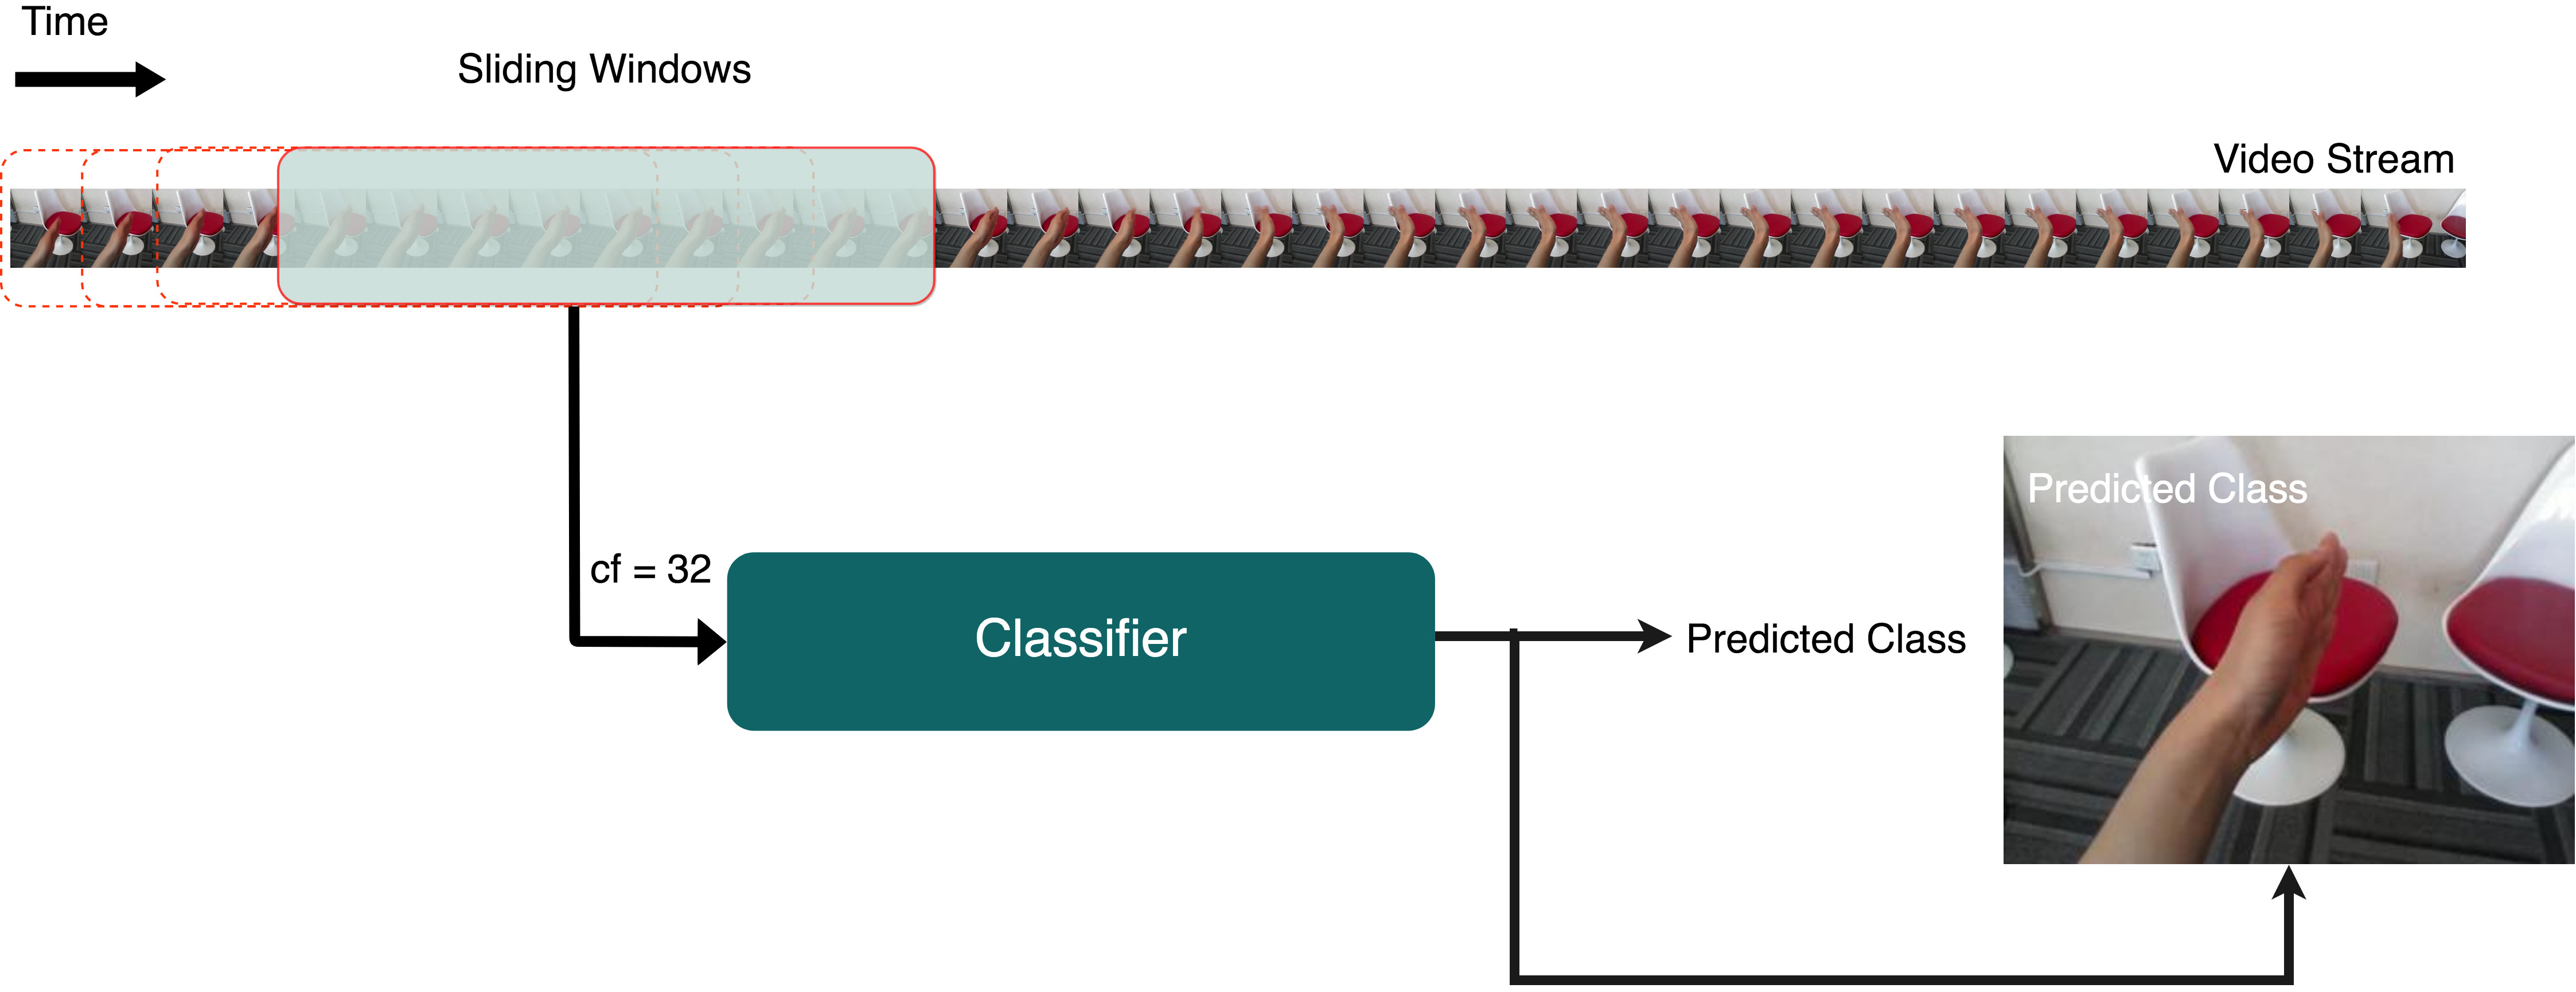
\includegraphics[width=1.0\linewidth]{figures/old_workflow}
	\caption{A basic approach of real-time gesture detection application.}
	\label{fig:old_workflow}
\end{figure}

Currently, one way of dealing with a real-time classification task could have been to run a trained model on a fixed size of a window of frames of an incoming video stream with an overlapping factor as shown in Figure \ref{fig:old_workflow}.  The overlapping strategy is essential because a gesture can start or end at the border of the window, and it is highly possible that the model would miss this.  Moreover, the timing of the detection/classification of gestures matters a lot in gesture recognition applications.   However, these models are not trained for such a scenario.  It is clear to say that frames in a window will often not be as clean as ones the model has been trained on. There could be frames that have no actions or maybe the action takes longer than it usually takes and the model will most probably miss-classify it.   Another drawback of this approach is that the model will activate more than once for the same gesture as the model go through on the same frames several times.  This brought up the following problems:
\begin{enumerate} 
\item We can never be sure when the true gesture starts since the beginning of many gestures can be very similar
\item We cannot be sure when it ends.
\item For one gesture we will have many activations.
\end{enumerate}
On the other hand,  computational resources do not need to be always used since the most of the time there is no any gesture performed in a real-time scenario.  Because of this,  we created a  two-models architecture where one light-weight model (detector) always runs and do binary classification if there is a gesture or not.   This model does not require a complicated structure most of the time since the task is more straightforward than classifying the gestures.   So if this model activates,  then the classifier will start processing. The second model (classifier) is a much more complex model than the detector because most of the resources will not be used if there is no gesture in the video stream.  After that, the classifier’s softmax outputs are post-processed to predict the outcome.  The whole structure is shown in Figure \ref{fig:workflow} (see Section \ref{sec:architecture}).\\

For the sake of eliminating these three problems above,  we propose a system has two models (detector and classifier), and a single-time activation strategy.   Figure  \ref{fig:probs} presents how decision mechanism has been done in the proposed system.\\

In the rest of this chapter,  datasets used in experiments are introduced, and then proposed network architecture is elaborated.\\
\clearpage
\section{Datasets}
\label{sec:datasets}
Vision-based human action and activity recognition tasks have an increasing trend among the computer vision community together with some applications like visual surveillance, video retrieval, and human-computer interaction.  In recent years,  more and more datasets are dedicated to human action/gesture recognition, and the use of these data sets allows us to compare different recognition systems performances.    Before the release of the  Kinetics  Human  Action  Video Dataset provided by Deepmind, research has mainly focused on learning and recognizing actions from two-dimensional (2D) approaches on frames \cite{vishwakarma_survey_2012,lim_fuzzy_2015,wang_recent_2003,guo_survey_2014}.  As a result of this,  there have been many publicly available  2D video datasets dedicated to action recognition. Review papers categorizing and summarizing their characteristics are available to help researchers in evaluating their algorithms  \cite{hassner_critical_2013,chaquet_survey_2013,ruffieux_survey_2014}.   The introduction of low-cost integrated depth sensors that can capture both RGB  (red,  green and blue) video and depth (D) information has significantly advanced the research of vision-based action recognition.   Since the first work reported in 2010 \cite{li_action_2010}, many benchmark datasets have been created to facilitate the development and evaluation of new algorithms based on 3D analysis on a stack of adjacent video frames, which is more reasonable for classification of time-related tasks such as action recognition.  On the other hand,  3D CNNs are proven to be more data-hungry in order to be trained.\\

Even though there are many vision-based datasets  available, not all of these datasets are suitable for our purpose since most of them are only providing the clips in which an action/gesture performed, which is not appropriate for training a real-time model that requires a continuous stream has regions with no action. Additionally, our research question requires a dataset to have the following attributes:
\begin{itemize}
\item To be \textbf{large enough} to train  a complex Deep Neural Network
\item Needs to be \textbf{challenging} concerning the number of gestures
\item Availability  of \textbf{no gesture part} in the videos to do continuous  classification
\item Allow us to \textbf{benchmark} our strategy and models.
\item Ability to \textbf{generalize} our approach
\end{itemize}

As a result of these prerequisites,  we evaluated proposed architecture on two dynamic hand gesture datasets:   1) EgoGesture dataset \cite{zhang_egogesture:_2018} and 2)Nvidia Dynamic Hand Gestures  Dataset  (annotated as nvGesture in this report)  \cite{nvidia_online_nodate}. \\

\subsection{EgoGesture Dataset}
\label{subsec:egogesture}
The dataset consists of videos from 50 subjects.  In total,  there are 2,081 RGB-D videos with 83 distinct dynamic or static gesture classes as shown in Figure  \ref{fig:egogesturesall}\cite{cao_egocentric_2017,zhang_egogesture:_2018}\footnote{\url{http://www.nlpr.ia.ac.cn/iva/yfzhang/datasets/egogesture.html}}.  On average each gesture class has 291 samples.\\
\begin{figure}[H]
	\centering
	\includegraphics[width=1\linewidth]{figures/Gestures_all}
	\caption{Eighty-three dynamic or static hand gesture classes in EgoGesture dataset.}
	\label{fig:egogesturesall}
\end{figure}

\begin{figure}[h]
	\centering
	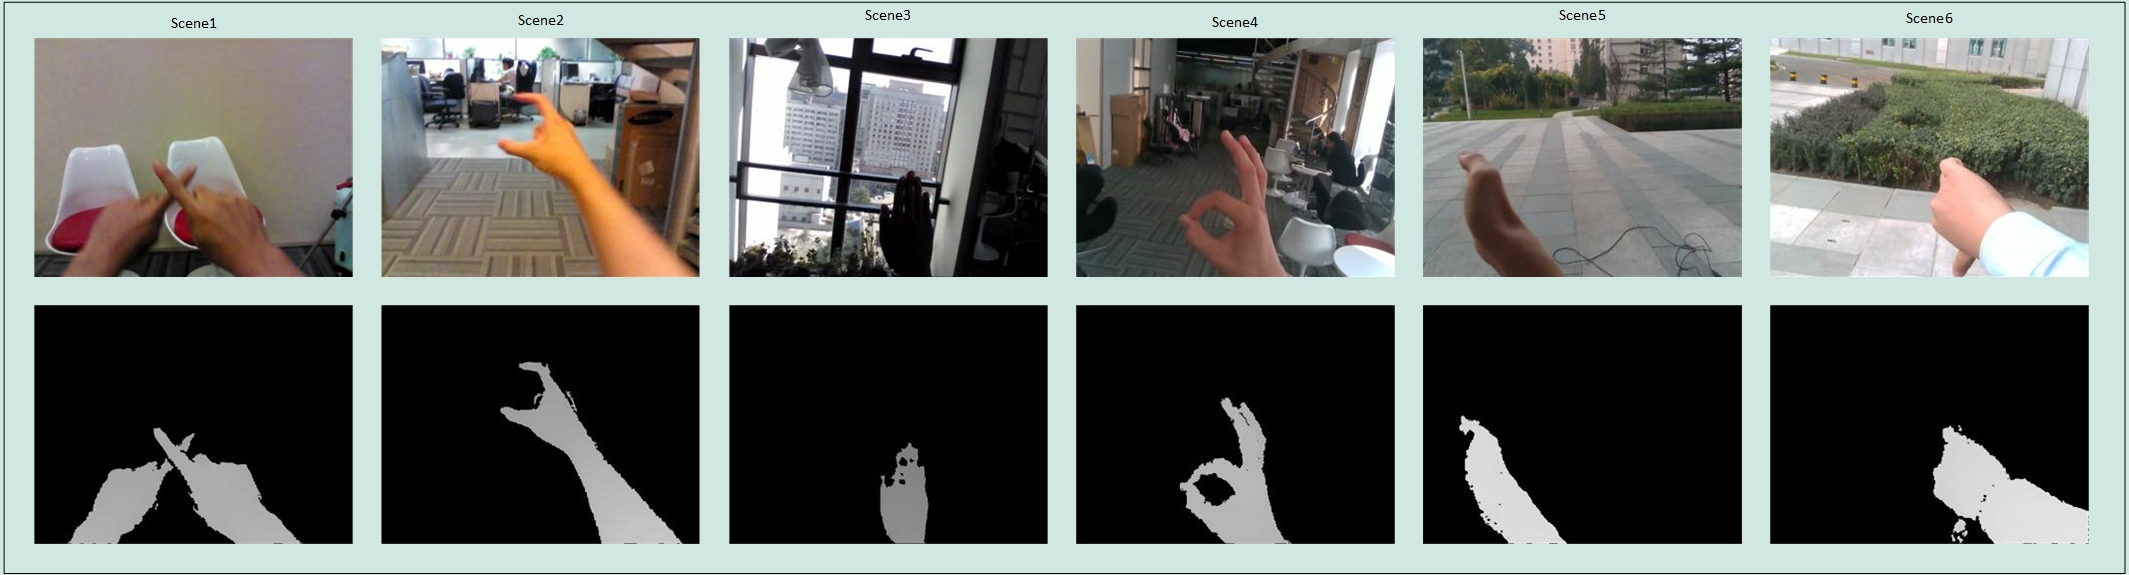
\includegraphics[width=1\linewidth]{figures/Scenes}
	\caption{Some gesture samples in 6 distinct scenes with different background and setting. Top and bottom samples are from RGB and Depth sensors, respectively} 
	\label{fig:scenes}
\end{figure}
The data is recorded in 6 different scenes while some of them are not stationary.  In \cite{zhang_egogesture:_2018,cao_egocentric_2017} each scene is described  as follows:
\begin{itemize}
\item the subject in a stationary state with a static clutter background
\item the subject in a stationary state with a dynamic background
\item the subject in a stationary state facing a window with drastic-changing sunlight
\item the subject in a walking state
\end{itemize}
and two outdoor scenes:
\begin{itemize}
\item the subject in a stationary state with a dynamic background
\item the subject in a walking state with a dynamic background.
\end{itemize}
The examples from the 6 scenes are illustrated in Figure \ref{fig:scenes}. 

Distribution of samples in each scene is illustrated in Figure \ref{fig:egogesturedist}. On the y-axis, the number of samples is shown for the corresponding subject, and each color represents the scene.  In total, we have 50 subjects (IDs from 1 to 50). Except for subjects with ID 3, 7, and 23, all other subjects recorded videos in all six scenes. It is clear that the distribution of scenes is quite balanced and on average each subject recorded about  500 samples.  This is quite important because it is harder to model to find patterns among scene, user and gestures.\\
\begin{figure}[h]
	\centering
	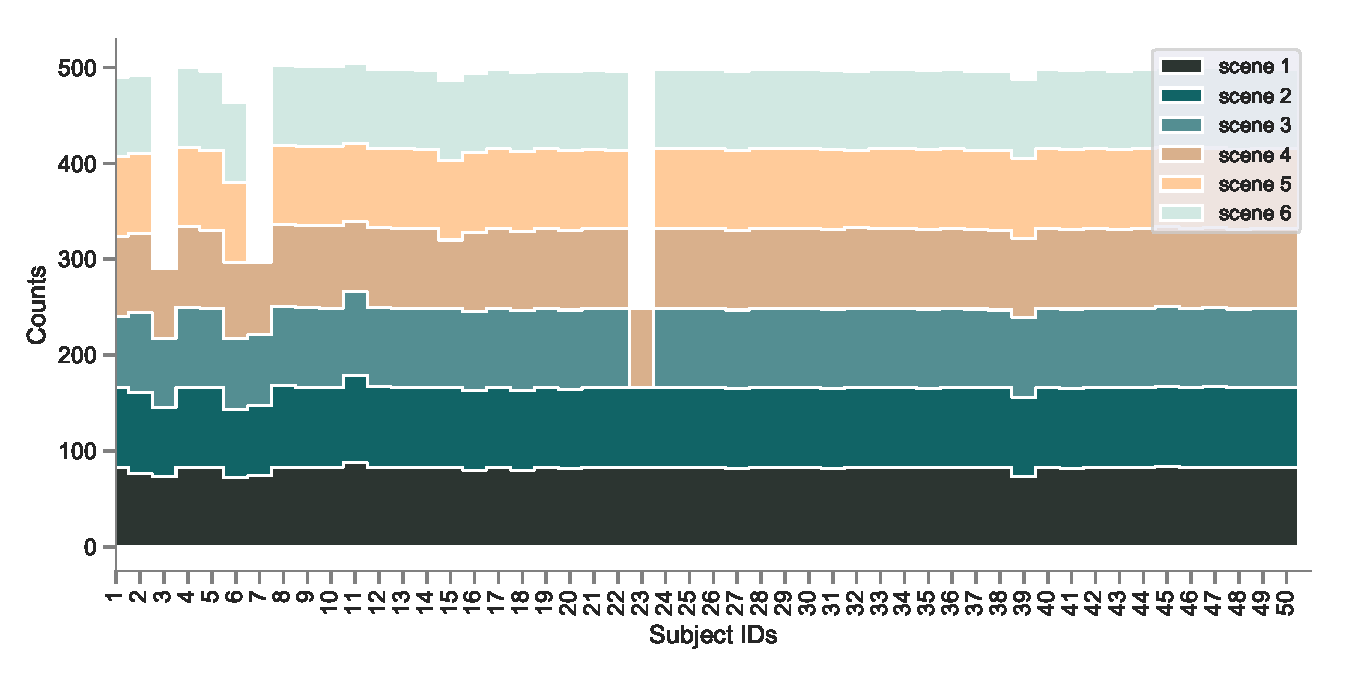
\includegraphics[width=1\linewidth]{figures/egogesturedist}
	\caption{The distribution of the gesture samples on each subject in EgoGesture dataset. The horizontal axis and the vertical axis indicate the subject ID and the sample numbers respectively.}
	\label{fig:egogesturedist}
\end{figure}

In the data collection process, Intel RealSense SR300 camera is used.  The camera is positioned on the head of each subject using a strap belt since one goal of this dataset is to capture the egocentric view of gestures.  The camera records 30 frames per second RGB-D modality videos with $640\times480$. Later in our experiments, we rescaled these images into $112\times112$. Each video consists of continuously performed gesture.  Thus, we are able to perform real-time classification experiments in continuous stream efficiently.  Besides, each clip has the gesture part of video  is labeled by providing start and end index of frames.  This allows us to train our offline models. \\

\begin{figure}[H]
	\centering
	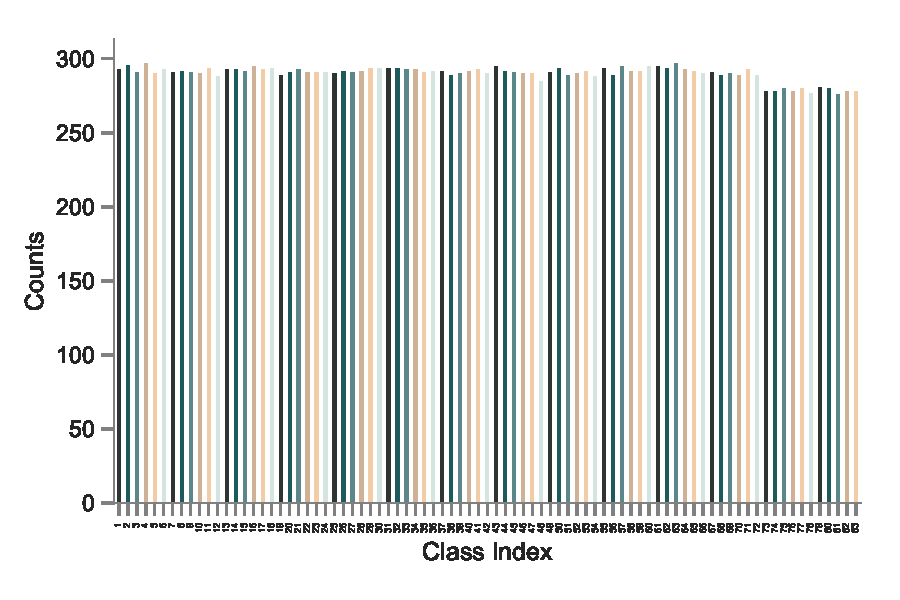
\includegraphics[width=0.8\linewidth]{figures/egogestureclassdist}
	\caption{Sample distributions per gesture class in the EgoGesture dataset.}
	\label{fig:egogestureclassdist}
\end{figure}

Figure \ref{fig:egogesturedist} shows the distribution of data over 6 scenes, and it is clear to say that it is quite balanced.  This is important for our training and evaluation phase.  Trained model can learn the structure of a scene more than the others, and this will mislead the model if the distribution is not balanced over the scenes.  On the other hand,  in Machine Learning (ML) task, the distribution of the classes/gestures plays an important role\cite{wei_role_2013}.  If dataset unbalanced and samples for some classes is more than samples from others in an exaggerated scenario, then the model will most probably only learn this class and always predict this class regardless of the input.   This is because,  in training, most of the loss will come from misclassification of those samples from majority classes, and model will be able to decrease the loss by correctly classifying only these samples but not others.   In the EgoGesture dataset, The classes are quite balanced as it is shown in Figure \ref{fig:egogestureclassdist}, And on average there are 291 gesture samples per classes.\\
\begin{figure}[h]%
\centering
\subfigure[]{%
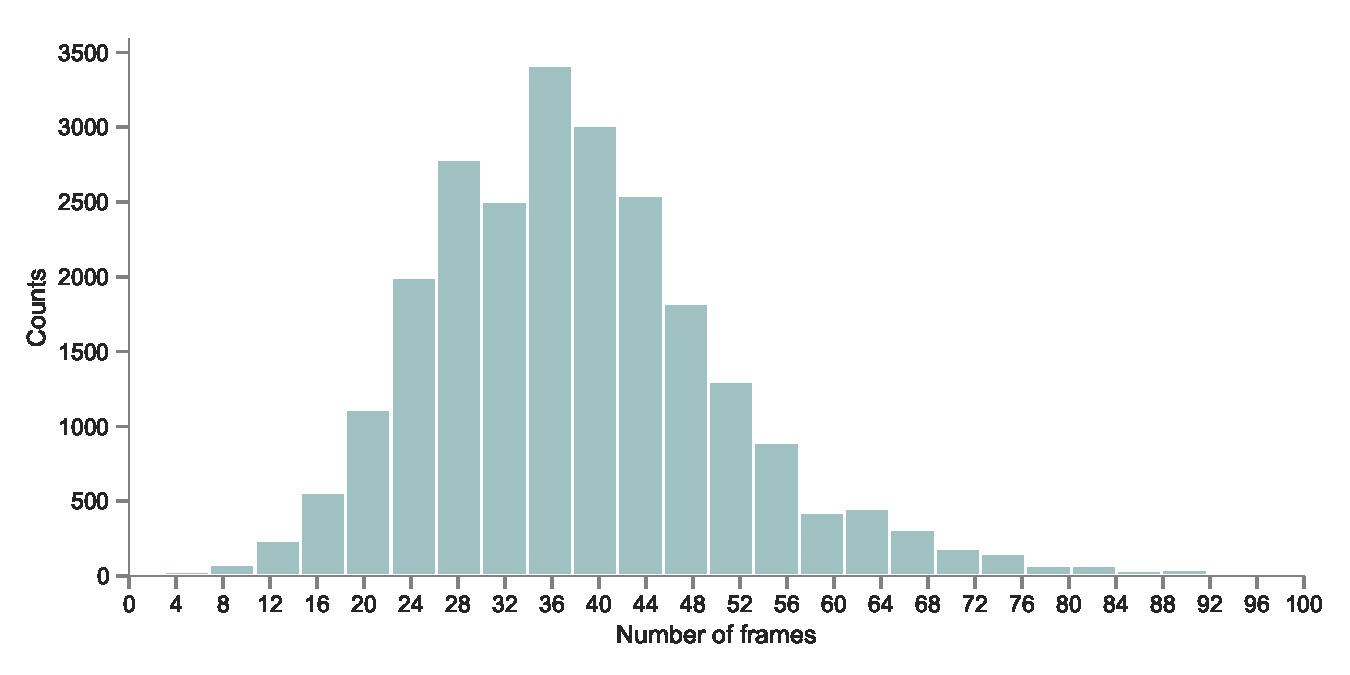
\includegraphics[height=0.25\linewidth]{figures/egogestureframesdist.pdf}}%
\label{fig:framedist1}%
\qquad
\subfigure[]{%
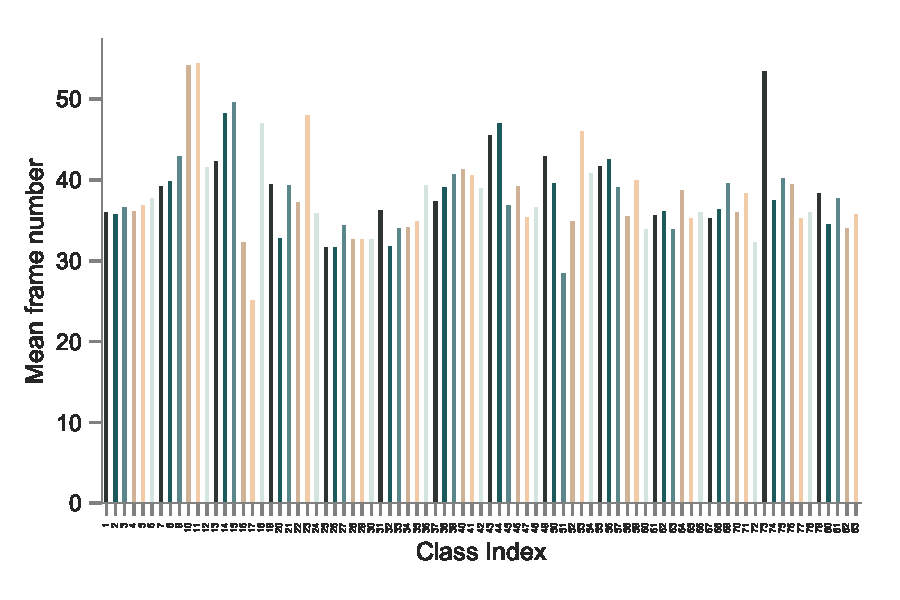
\includegraphics[height=0.25\linewidth]{figures/egogestureframedistperclass}}%
\caption{(a) Distribution of the number of frames per gesture. 
(b) Distribution of the number of frames for each gesture class in the EgoGesture dataset. }
\label{fig:egogestureframeall}
\end{figure}

In vision-based gesture recognition tasks, the number of frames per gesture plays a vital role in the decision of hyperparameters for 3D kernels.  In Figure  \ref{fig:egogestureframeall} (a),  it is shown that the number of frames per gesture across EgoGesture dataset has a Gaussian-like distribution whose mean is 38.4. The min and max number of frames are 3 and 196 respectively.  In this figure, however, we used samples in range 0-100, in which 99\% of the data lies, for the sake of better view of the distribution. There are only 37 samples which have less than eight frames and 79 samples with more than  100 frames. We realized that gesture with id 17, which is ”sweep diagonal” is mostly performed less than eight frames.  So  the mean number of frames across gestures is investigated, see Figure \ref{fig:egogestureframeall} (b). There is no any gesture stands out drastically from others.   Thus,  it is safe to assume the number of frames per gesture is not so much dependent on gesture class. \\

\subsection{NVIDIA Dynamic Hand Gestures Dataset}
\label{subsec:nvidia}
\begin{figure}[H]
	\centering
	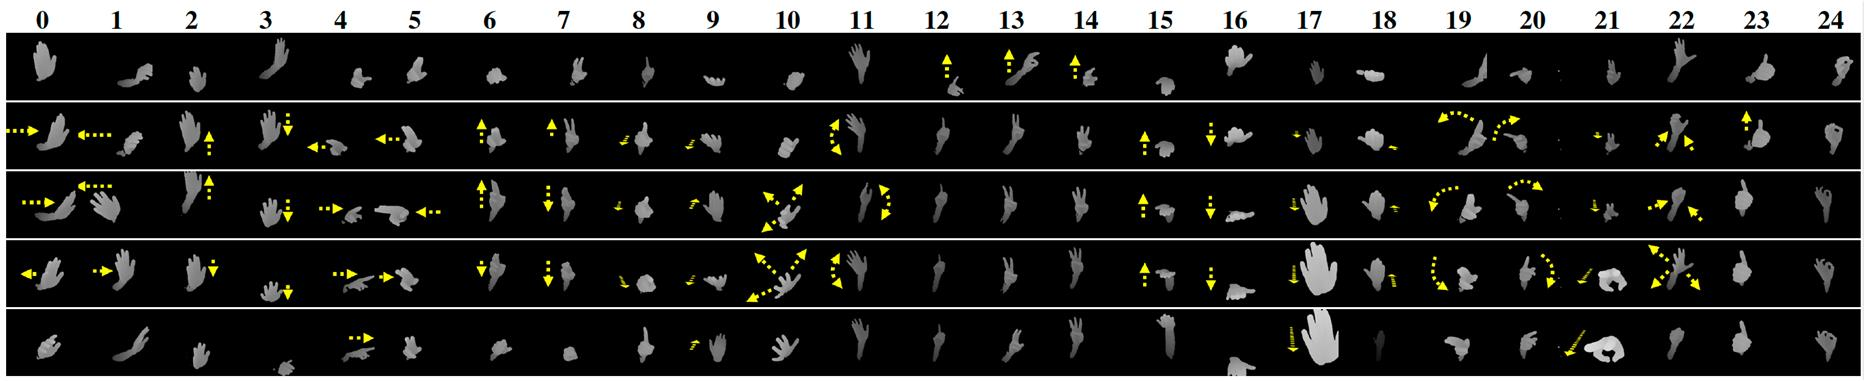
\includegraphics[width=1\linewidth]{figures/nvidia_classes_all}
	\caption{NVIDIA Dynamic Hand Gesture Dataset (nvGesture) classes. In total , there are twenty-five dynamic hand gestures (0-24) and each column represents each one of them. In bottom rows, yellow arrows illustrate the movement of hands. (This figure is from Molchanov et al. \cite{molchanov_online_2016} and more detailed information can be found there)}
	\label{fig:nvgesturesall}
\end{figure}

In the nvGesture dataset, there are in total 1050 video recordings for training and 482 recordings for testing from 20 different subject performing in a car simulation environment with different lightening scenarios. It includes 25 distinct gestures, shown in Figure \ref{fig:nvgesturesall}, while 6 of them being static gestures. Besides, the start and end frame of each gesture clip in nvGesture are not precisely cropped while each is represented by exactly 81 frames. Each gesture class has on average 61.2 recordings as it is shown in Figure \ref{fig:nvidiaclassdist}, which is much less than the average number of samples (291) per a gesture class in the EgoGesture. Moreover, Figure \ref{fig:nvidiaclassdist} illustrates the sample distribution for each classes, and it is clear to say that the dataset has a balanced class distribution which is critical in the training. \\
\begin{figure}[h!]
	\centering
	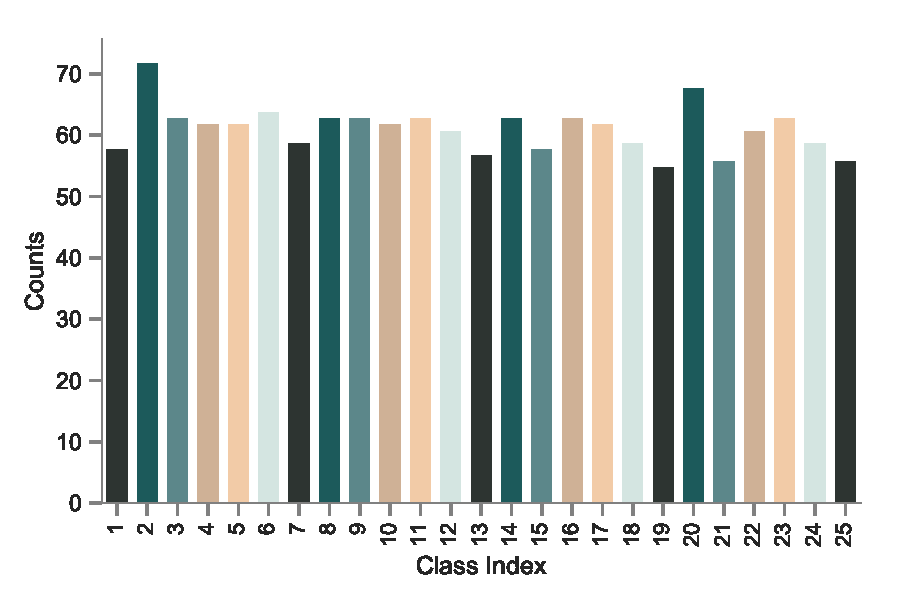
\includegraphics[width=0.5\linewidth]{figures/nvidiaclassdist}
	\caption{Sample distributions per gesture class in the nvGesture dataset.}
	\label{fig:nvidiaclassdist}
\end{figure}

In the nvGesture dataset, a SoftKinetic DS325 sensor was used to capture front view color and depth videos, and a DUO 3D camera was used to record stereo IR (left, disparity). Both cameras capture $320\times240$ pixels at 30 frames per second (fps) as it is introduced in \cite{molchanov_online_2016}. Overall, it contains optical flow and 4 other modalities: RGB, depth, IR-left, and IR-disparity. In our analysis,  we only used first view  RGB and depth modality videos  as it is more discriminative and natural view of the task. \\  

\section{Architecture}
\label{sec:architecture}
\begin{figure}[h!] 
	\centering
	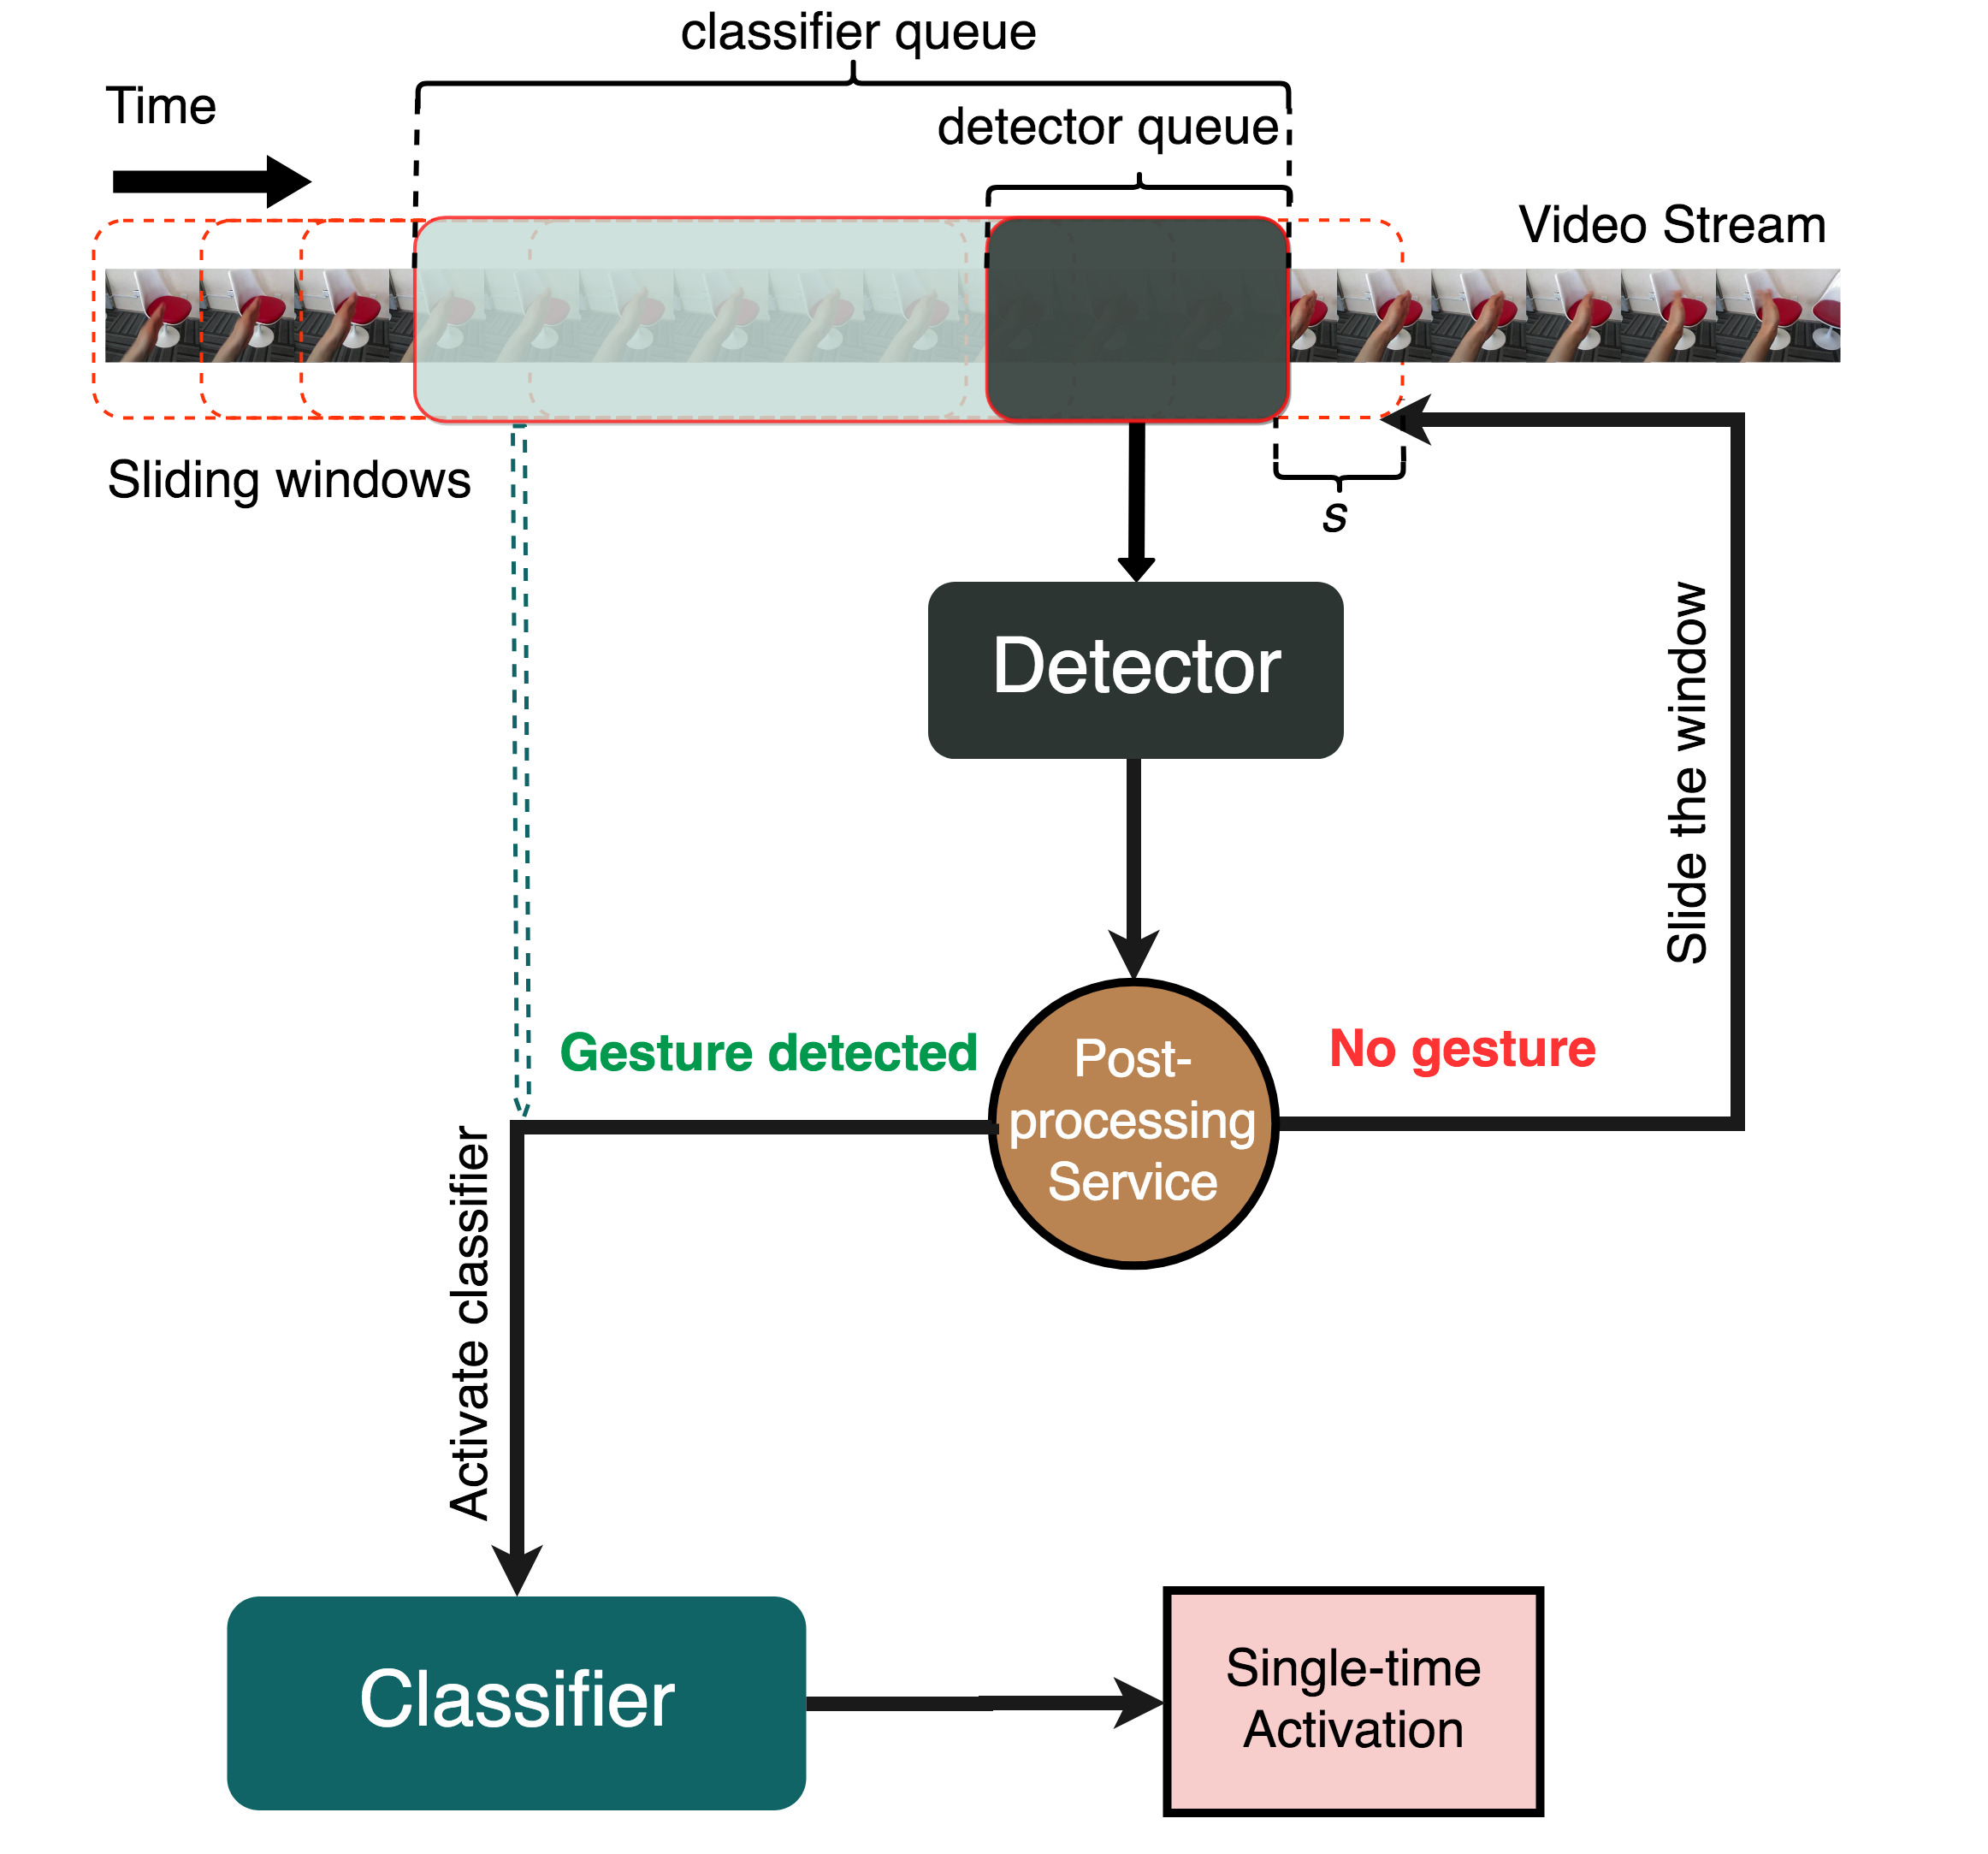
\includegraphics[width =0.9\textwidth]{figures/arch}
	\caption{The general workflow of the proposed two-model hierarchical architecture. Sliding windows with stride \textit{s} run through incoming video frames where detector queue placed at the very beginning of classifier queue. If detector recognize an action/gesture then the classifier is activated. Both detector and classifier outputs are post processed for a more robust performance, and decision is made using single-time activation block where only one activation occurs per performed gesture.}
	\label{fig:workflow}
\end{figure}

In this section, we elaborate on our two-model hierarchical architecture that integrates any state-of-the-art models into  real-time gesture recognition applications as efficiently as possible. After introducing two-model hierarchical architecture, training details are described. And finally, we give a deep understanding into the used post processing strategies that allow us to have single-time activation per gesture in real-time. \\

Recently, with the availability of large datasets, CNN based models have proven their ability in action/gesture recognition tasks. 3D CNN architectures especially stands out for video analysis since they make use of the temporal relations between frames together with their spatial content. However, there is no clear description of how to use these models in a real-time dynamic systems. With our work, we aim to fill this research gap.\\

Figure \ref{fig:workflow} shows illustrates the used workflow for an efficient real-time recognition performance using a sliding window approach. In contrary to offline testing, we do not know when a gesture starts or ends. Because of this, our workflow starts with a detector which is used as a switch to activate classifier if a gesture gets detected. Our detector and classifier models are fed by a sequence of frames with size $m$ and $n$, respectively such as $n \ll m$ with an overlapping factor as shown in Figure \ref{fig:workflow}. The stride used in the sliding window is $s$ and it is same for both the detector and the classifier. Although higher stride provides less resource usage, we have chosen $s$ as 1 since it is small enough not to miss any gestures and allows us to achieve better performance. In addition to the detector and classifier models, one post-processing and one single-time activation service is introduced to the workflow in order to achieve single-time activation per gesture. In the next parts, we are going to explain these blocks in detail.\\

As the overall accuracy of our system highly depends on the performance of the detector, we require the detector to be robust and accurate in detection of true positives, meaning that it must have high recall value.  For the sake of the former, detector runs on a smaller number of frames than classifier which we refer to as detector queue.   For the latter, detector queue is placed on the very beginning of classifier queue as shown in Figure \ref{fig:workflow}. Additionally,  we use some common filters like median,  moving average or exponentially weighted moving average in the post-processing service in order to clear out miss classifications.  This is not required for offline testing.   However, in online testing, we can make use of consecutive prediction scores of the models and allow the model to activate only once per gesture as we are using sliding windows with a stride length on the incoming video data.   We believe that this is the first work that shows how to use such post-processing techniques in vision-based gesture recognition tasks.\\
\begin{figure}[H]
	\centering 
	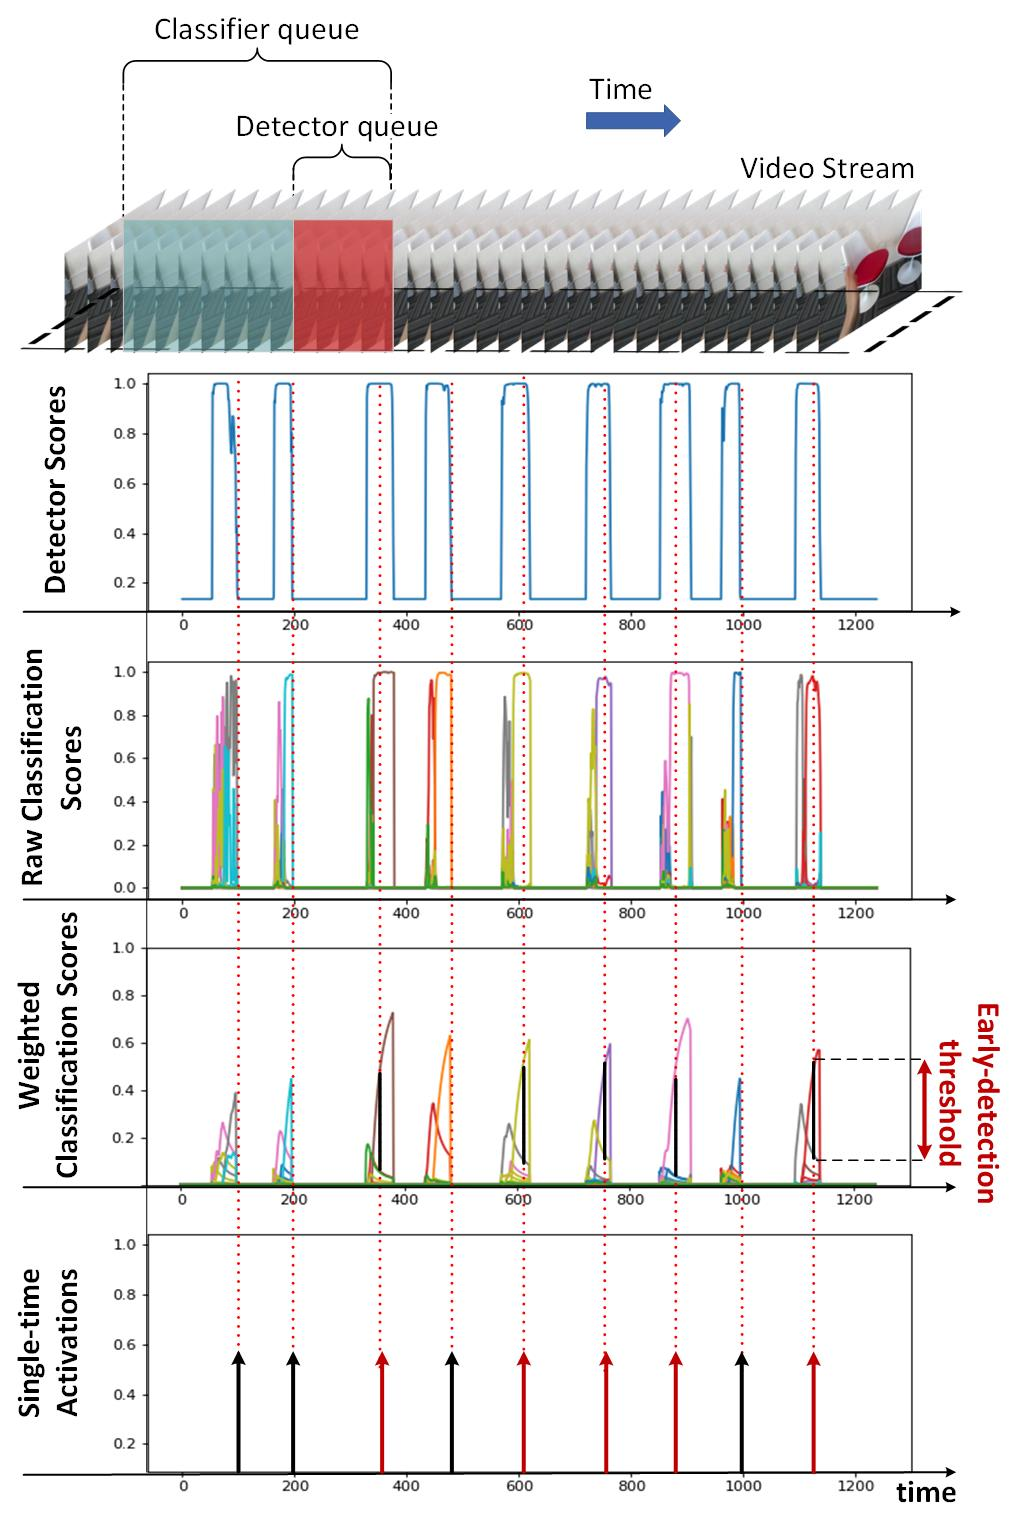
\includegraphics[width=0.8\textwidth]{figures/probs}
	\caption{Proposed pipeline illustrations for real-time gesture recognition. When we run our proposed structure over an incoming video stream by sliding one frame at each iteration, these results are achieved. First figure shows detector probability scores for class 1 (\textit{gesture}), second figure illustrates each classes classification score with different colors, third one is weighted-average of classification scores with weight function $W(x) = 1/(1+\exp^{-0.2\times(x-9)})$ where $x$ is the iteration index, and the bottom one illustrates single-time activations such that red arrow represents early detection and black one is for detection after gesture ends.}
	\label{fig:probs}
\end{figure}

Figure \ref{fig:probs} shows the transformation of the classifiers probability scores through the proposed architecture shown in Figure \ref{fig:workflow}. The difference between the weighted-average of the scores and the raw scores plots proves that the true gesture can be emphasized and detected more precisely as the true information in the gesture lies at the mid-late range of it. Additionally, the early detection strategy is shown with the help of an threshold level. Finally, the bottom image shows the activations of each gestures in real time evaluation (red colored arrows represent early detections). In total we are able to successfully detect all true classes for this sample (EgoGesture dataset, Subject 4, Scene 2 and recording 5), while 5 of them being early detected.\\
\subsection{Detector}
\label{subsec:detector}
\begin{figure}[t!]
	\centering
	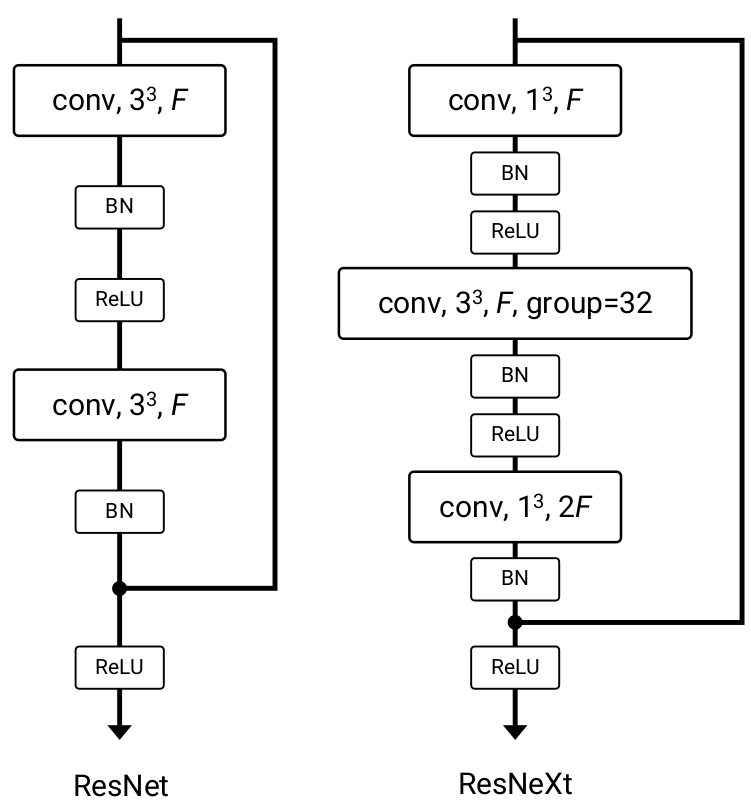
\includegraphics[width=0.5\textwidth]{figures/blocks}
	\caption{ResNet and ResNeXt blocks used in the detector and classifier architectures.}
	\label{fig:blocks}
\end{figure}
Detector runs on the images in the detector queue in every iteration, and the purpose of this model is to detect if any action is performed,  ”1” for \textit{gesture} and ”0” for \textit{no gesture}.  Its main and only role is to act as a switch for the classifier model, meaning that if the detector predicts ”1” classifier is activated and fed by frames in its own window. However, it is possible that for some frames there is no hand present and it can predict \textit{no gesture} while a gesture being performed.  In order to decrease this possibility, we post-process the output probabilities, and after that, we set a threshold $d_{th}$ for the consecutive number of \textit{no gesture} predictions to deactivate classifier.\\

The purpose of the detector is to distinguish between \textit{gesture} and \textit{no gesture} classes by running on a sequence of images that detector queue masks at every iteration. Its main and only role is to act as a switch for the classifier model, meaning that if it detects a \textit{gesture}, then classifier is activated and fed by the frames in classifier queue.\\

As the overall accuracy of this system highly depends on the performance of detector, we require the detector to be (i) robust and (ii) accurate in detection of true positives, meaning that it must have high recall value. For the sake of the former, detector runs on smaller number of frames than classifier which we refer as detector and classifier queues. For the latter, detector queue is placed on the very beginning of classifier queue as shown in Figure \ref{fig:workflow}, and this enable the detector to activate the classifier whenever a gesture starts regardless of the gesture duration.\\ 
\begin{table}[t!]
	\centering
	\begin{tabular}{c|c|c|c}
	\hline
	\textbf{Layer}    & \textbf{Output Size}   & \textbf{ResNeXt-101}  & \textbf{ResNet-10} \\ \hline
	conv1    & L x 56 x 56   & \multicolumn{2}{c}{3x7x7, stride (1, 2, 2)}                                                                 \\ \hline
	conv2\_x & L x 56 x 56   & N:3, F:128                                            & N:1, F:16                                            \\ \hline
	conv3\_x & L/2 x 56 x 56 & N:24, F:256                                           & N:1, F:32                                            \\ \hline
	conv4\_x & L/4 x 56 x 56 & N:36, F:512                                           & N:1, F:64                                            \\ \hline
	conv5\_x & L/8 x 56 x 56 & N:3, F:1024                                           & N:1, F:128                                           \\ \hline
         & 1 x 1 x 1     & \multicolumn{2}{c}{\begin{tabular}[c]{@{}c@{}}global average pooling,\\ fc layer with softmax\end{tabular}} \\ \hline
	\end{tabular}
    \caption{Detector (ResNet-10) and Classifier (ResNeXt-101) architectures. F corresponds to the number of feature channels in the blocks shown in Figure \ref{fig:blocks}, N is the number of blocks in corresponding layer, and L is the number of frames fed to the model.}
	\label{tab:architecture}
\end{table}

%Additionally, we used some common filters (moving median, moving average and exponentially-weighted moving average) in the post processing service in order to clear out miss classifications in online testing. This filtering strategy allowed us to make use of consecutive prediction scores of the models. We believe that this is the first work that shows how to use such post-processing techniques in vision-based gesture recognition tasks.

The proposed detector architecture is build upon two critical assumptions: \textit{(1)} The detector should be a lightweight model since it is running continuously, and \textit{(2)} the detector should not miss any \textit{gesture} classes. For the sake of \textit{(1)}, we focused on a relatively shallow 3D CNN architecture, and decided to use ResNet-10 with reduced number of features in each layer. ResNet-10 architecture is given in Table \ref{tab:architecture} which uses the ResNet block given in Figure \ref{fig:blocks}. In order to achive \textit{(2)}, the detector model is trained with a weighted-cross entropy loss in order to decrease the likelihood of false positives. Class weights for class \textit{no gesture} and \textit{gesture} is selected as 1:3, respectively as our experiments showed that this proportion is sufficient to have 98+\% and 97+\% recalls in in EgoGesture and nvGesture datasets, respectively. Besides that, we post-process the output probabilities, and set a counter for the consecutive number of \textit{no gesture} predictions in decision of deactivating classifier. As an input to our detector,We have analyzed the input modalities of RGB, Depth and the data level fusion of both of them (RGB-D) \cite{kopuklu2018motion}. \\
\subsection{Classifier}
\label{subsec:classifier}
In computer vision (CV) area, gesture recognition has been one of the main tasks, and researchers have come quite a way since the beginning of the CV area. Most of these researches are about achieving the highest accuracy on some selected benchmark datasets.  Rarely,  the focus is on how to use these models in a real-time scenario.  In this work, we aim to integrate these developed models which have reasonable accuracy rate into a real-time application.\\

Since we do not have any limitation regarding the size or complexity of the model, any architecture with good performance in this task can be selected for classification.  This lead us to use two recent 3D CNN architectures (C3D \cite{tran_learning_2014}, and ResNext-101 \cite{he_deep_2015}) as our classifier model.  However, it is important to note that our architecture is independent of the model type.\\

Since the invention of \textbf{LeNet-5} \cite{lecun_gradient-based_1998} in LeCun et al.  which is considered as the first Convolutional neural network (CNNs) architecture, CNNs has found its position as the most successful method to learn, recognize patterns from images.  In this section, we first introduce the underlying architecture of C3D and one of its variant (called ResNext-101 \cite{xie_aggregated_2016}) that we used as a classifier in this work because we mainly focused on these two methods in this thesis and then explain our training strategies for the classifier.\\

For C3D model, we have used the exact same model as in \cite{tran_learning_2014} but the last two fully connected layers where we have used 2048 nodes instead of 4096. For ResNeXt-101, we have followed the guidelines of \cite{hara3dcnns} and chose the model parameters as given is Table \ref{tab:architecture} with ResNeXt blocks as in Figure \ref{fig:blocks}. The most basic ResNet block has two convolutional layers followed by a ReLU activation, and there is a connection between input and output after which there is another  ReLU operation.   This structure is first introduced in \cite{he_deep_2015}, and it allows for training more than  100 layers.   This revolutionized Computer  Vision/ Deep Learning community as training deep networks without overfitting is one of the main challenges.  In \cite{he_identity_2016}, researchers achieved to train even 1001-layered ResNet.  Because of its appealing results in many tasks,  ResNet quickly became popular in the research community. There are many variants of ResNet developed in 3 years by changing the structure of the residual block. One of the most successful ones is called ResNext.\\

As the number of parameters for 3D CNNs are much more than 2D CNNs, they require more training data in order to prevent overfitting. Because of this reason, we pretrained our classifier structures first on Jester dataset \cite{twentybn_20bn-jester_nodate}, which is the largest publicly available hand gesture dataset, and then fine tune our model by using this pretrained model as initialized.  This approach increased the accuracy and shortened the training duration drastically. \\

\textit{Training Details: } We used stochastic gradient descent (SGD) with Nesterov momentum = 0.9, damping factor = 0.9, and weight decay = 0.001 as optimizer. After pretraining on Jester dataset, the learning rate is started as 0.01, and divided by 10 at $10^{th}$ and $25^{th}$ epoches.\\

For regularization, we used a weight decay ($\gamma = 1 \times 10^{-3}$) is applied on all the parameters of the network. We also used dropout layers in C3D and several data augmentation techniques through out training.\\

In case of augmentation methods, three methods were used: (1) Each image is randomly cropped with size $112 \times 112$ at corners such that one of 4 corners is selected uniformly. (2) Spatial elastic displacement with $\alpha = 1$ and $\sigma = 2$ is applied after cropping images. For temporal augmentation , on the other hand, (3) we randomly select consecutive frames with input sample duration from the entire gesture videos. If the sample duration is more than number of frames in target class, we append frames starting from very first frame in a cyclic fashion. We also normalized the images into 0-1 scale using mean and standard deviation of the whole training sets in order to force models to learn faster.\\

During offline and online testing, we scaled images into $112 \times 112$ and then only normalization is performed for the sake of consistency between training and testing. The same training details are used for detector and classifier models.\\
\clearpage
\subsection{Post-processing}
\label{subsec:pp}
\begin{figure}[b!]
	\centering
	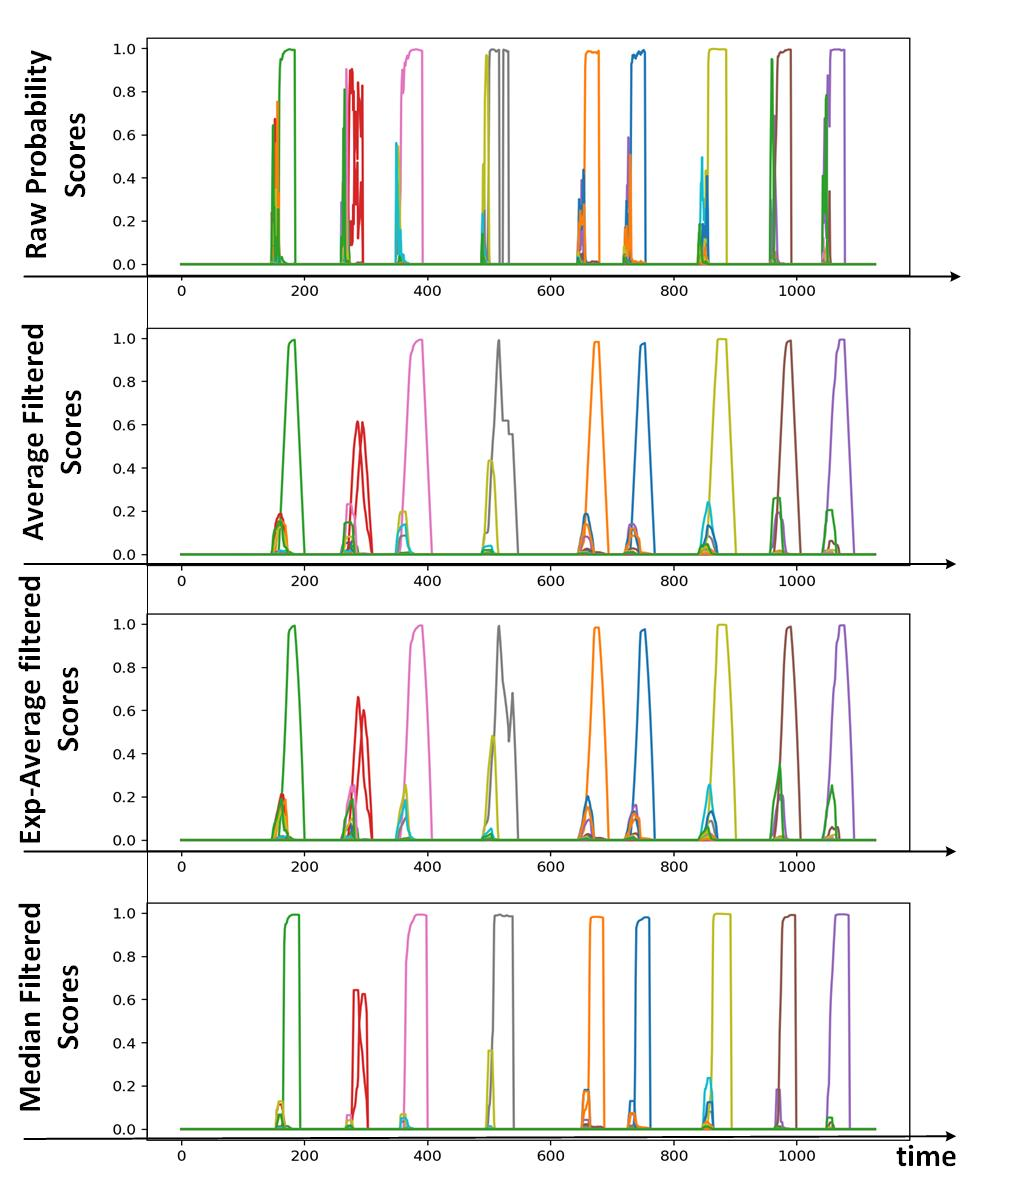
\includegraphics[width=0.8\textwidth]{figures/post}
	\caption{An illustration of the effect of post-processing filters on classification scores of each class: raw, uniformly-averaged, weighted-averaged and median filtered probability scores from top to bottom.}
	\label{fig:post}
\end{figure}

In dynamic hand gestures, it is possible that the hand gets out of the camera view  while performing gesture. Even though previous predictions of the detector are correct, any misclassifications reduce the overall performance of the proposed architecture. In order to make use of previous predictions, we add the raw softmax probabilities of the previous detector predictions into a queue ($q_k$) having a size of $k$, and apply filtering on these raw values resulting in final detector decisions. With this approach, detector increases its confidence in decision making, and clears out most of the misclassifications in consecutive predictions. The size of the queue ($k$) is selected as 4, which achieved the best results for stride $s$ of 1 in our experiments. \\

We have applied $(i)$ average, $(ii)$ exponentially-weighted average and $(iii)$ median filtering separately on the values in $q_k$. While average filtering simply takes the mean value of the $q_k$, median filtering takes median. Exponentially-weighted average filtering, on the other hand, uses weighting function of  $w_i = \exp^{-{{(1-(k-i))}/k}}$ where $i$ stands for the index of $i^{th}$ previous sample and satisfies $0 \leq i < k$, and $w_i$ is the weight for the $i^{th}$ previous sample. For better understanding, we tested different filtering approaches on the multi-classification task, shown in Figure \ref{fig:post}. \\



%These methods cancels out most of the miss classifications. We observed that median filter forces the true class stands out even more and clears of misclassifications due to the camera view. As a result, we used median filtered scores with queue size $k = 2$ in our architecture. In \cite{molchanov2016online}, a similar results are achieved by training the model with CTC loss; however, in Figure SOMETHING!!!!!, it is shown that we can force the true gestures stands out even more with much less effort.

\begin{figure}[b!]%
\centering
\subfigure[]{%
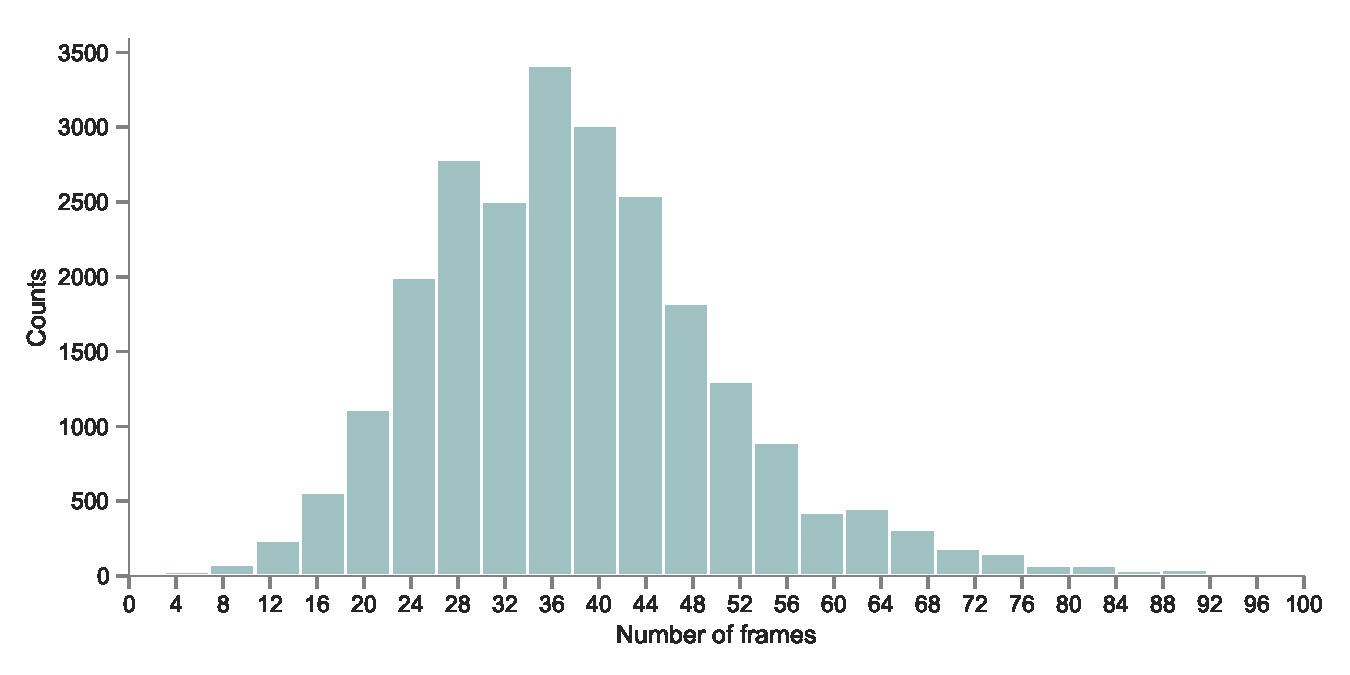
\includegraphics[width=0.45\linewidth]{figures/egogestureframesdist}}%
\label{fig:egoframe}%
\qquad
\subfigure[]{%
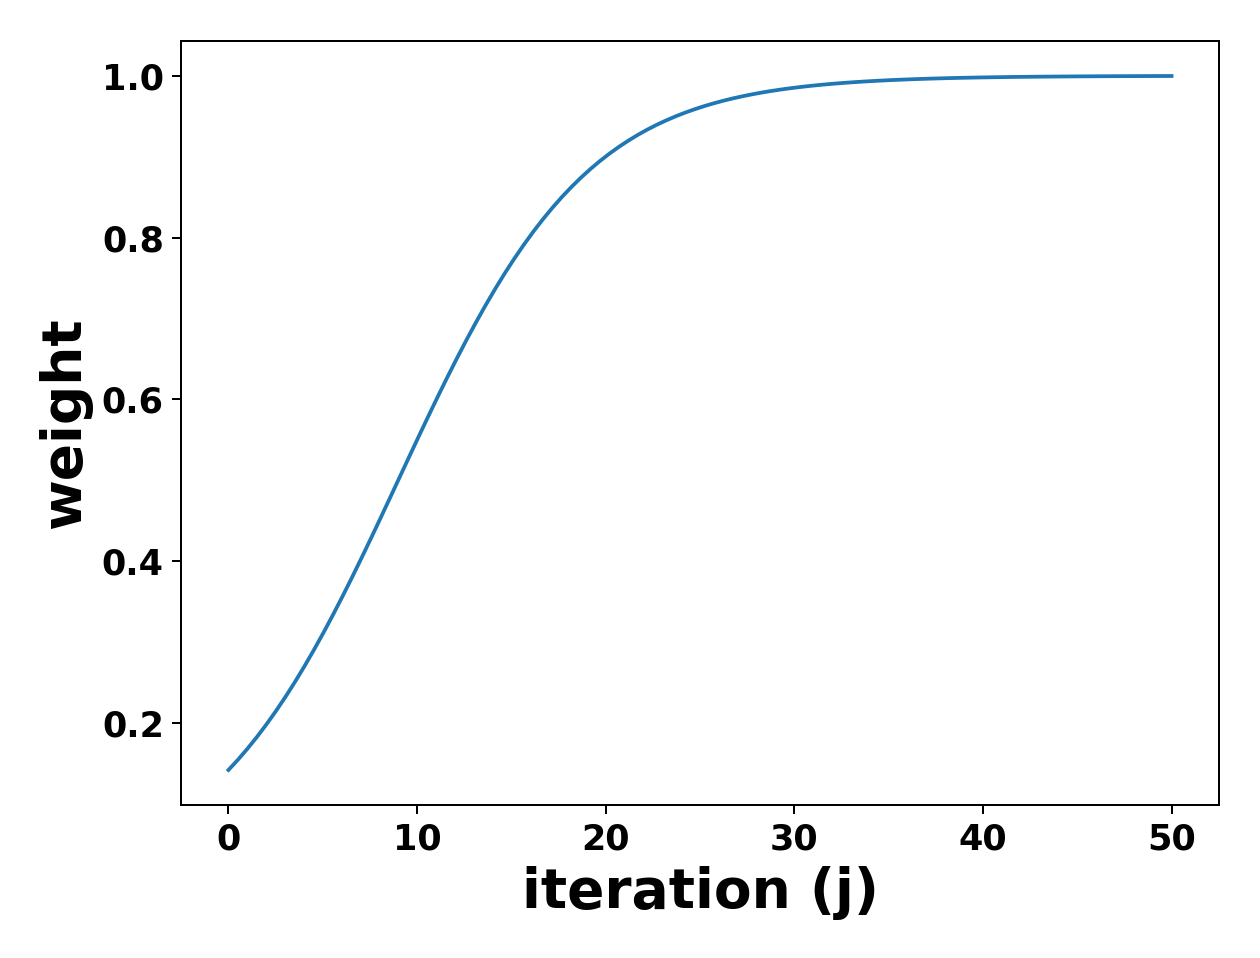
\includegraphics[width=0.45\linewidth]{figures/sigmoid.png}}%
\caption{(a) Histogram of sample durations (b) Sigmoid-like weight function used in single-time activation according to the Equation \eqref{eq:weight}.}f
\label{fig:sigmoid}
\end{figure}


\subsection{Single-time Activation}
\label{subsec:sta}
In real-time gesture recognition systems, it is extremely important to have smaller reaction time and single-time activation for each gesture. Gavrila et al.\cite{Gavrila1999TheVA} states that dynamic gestures have \textit{preparation}, \textit{nucleus} and \textit{retraction} parts. Out of all parts, nucleus is the most discriminative one, such that we can decide which gesture is performed even before it ends.  \\

Single-time activation is achieved through two level control mechanism. Either a gesture is detected when a confidence measure reaches a threshold level before gesture actually ends (early-detection), or the gesture is predicted when the detector deactivates the classifier (late-detection). In late-detection, we assume that the detector should not miss any gesture since we assured that detector has a very high recall rate. \\
\begin{figure}[t!]
	\centering
	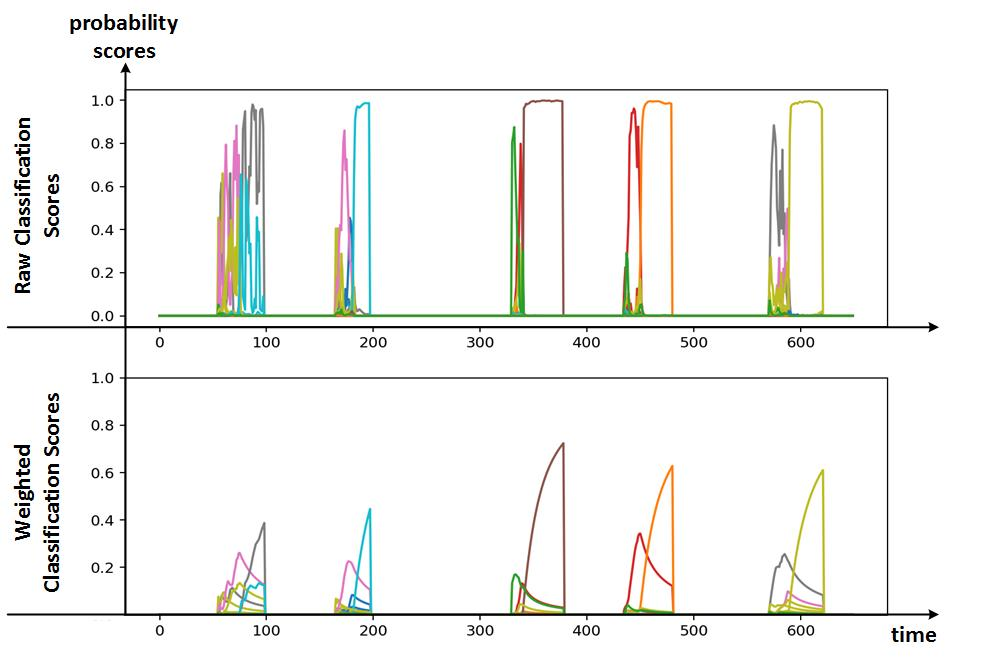
\includegraphics[width=\textwidth]{figures/weight_effect.jpg}
	\caption{Raw and weighted classification scores(top and bottom respectively). In top image we can see a lot of noise in the beginning of all gestures; however, near to the end of each gesture the classifier classify with more confidence. as The bottom image shows that we are able to cancel out this noise part through assigning smaller weights to the beginning part of gestures.}
	\label{fig:weight}
\end{figure}

The most critical part of the early-detection is that, the gestures should be detected after their nucleus parts for a better recognition performance. Because, several gestures can contain a similar preparation part which creates an ambiguity at the beginning of the gestures, as can be seen on the top graph of Figure \ref{fig:weight}. Therefore, we have applied weighted-averaging with a weight function as in Figure \ref{fig:sigmoid} (b), and its formula is given as,

\begin{equation}
    \label{eq:weight}
    w_j = \frac{1}{(1+\exp^{-0.2\times(j-t)})}
\end{equation}
    
\noindent where $j$ is the iteration index of an active state, at which a gesture is detected, and $t$ is selected as 9 by using the following formula,

\begin{equation}
    t = \frac{f}{2 \times s}
\end{equation}

\noindent where $f$ corresponds to the mean duration of the gestures(in number of frames) and $s$ is the stride length. This parameters allow us to have 0.5 and higher weights in nucleus part of the gestures on average. Figure \ref{fig:weight} shows the probability scores of five gestures over each iteration and their corresponding weighted-averages. It can easily be observed that we successfully cleared out the ambiguity of the classifier at the preparation part of the gestures.\\
\begin{algorithm}[t!]
	\renewcommand{\algorithmicrequire}{\textbf{Input:}}
	\renewcommand{\algorithmicensure}{\textbf{Output:}}
	\caption{Single-time activation in real-time gesture recognition }
    \centering
	\label{online_testing}
	\begin{algorithmic}[1]
		\Require Incoming frames from video data.
		\Ensure Predicted gestures.
		\For{each "frame-window" $w_i$ of length $m$}
		\If{a gesture is detected}
		\State{state $\leftarrow$ "Active"}
        \State {$\alpha \leftarrow probs_{j-1}\times(j-1) $}
        \State {$mean_{}probs = (\alpha + w_j\times probs_{j})/j$ }
        \State {$(max_1,max_2)=\max\limits_{gesture}{[mean_{}probs]_2}$ }
        \If{$(max1 - max2) \geq \tau_{\mathbf{early}}$}
        \State {\textit{early-detection} $\leftarrow$ "True"}
        \State \Return {gesture with $max_1$}
        \EndIf
        \State {$j \leftarrow j + 1$}
        \EndIf
        \If{the gesture ends}
        \State{state $\leftarrow$ "Passive"}
        \If{\textit{early-detection} $ \neq$ "True" \& $max_1 \geq \tau_{\mathbf{late}} $}
        \State \Return {gesture with $max_1$}
        \EndIf
        \EndIf
        \State {$i \leftarrow i + 1$}
        \EndFor
	\end{algorithmic}
\end{algorithm}

With this weighted-averaging strategy, we force our single-time activator to make decision at mid-late part of the gestures after capturing their nucleus parts. On the other hand, we need a confidence measure for early-detections in real-time since the duration of gestures varies. Hence, we decided to use the difference between weighted average scores of each classes as our confidence measure for early-detection. If detector switched on classifier, weighted average of probabilities for each class is calculated at each iteration. If the difference between two highest average probabilities is more than a threshold $\tau_{early}$, then early-detection is triggered; otherwise, we wait for the detector to switch off the classifier and the class with highest score above $\tau_{late}$ is predicted as late-detection. Details for this strategy can be found in Algorithm \ref{online_testing}. In our experiments we decided to fix $\tau_{late} = 0.15$ for simplicity. Also, its value is not so much important when the detector works well.\\

\section{Evaluation of Activations}
%As opposed to offline testing that uses standard metrics like accuracy,  recall, precision, etc...,  in online (real-time) testing evaluation of results is not only about how many of the gestures are correctly predicted but also many predictions.  Because of this reason, we used Levenshtein distance as our distance measure in online experiments evaluation. The Levenshtein distance is a sequence metric that measures the distance between sequences by counting the number of item-level changes (insertion,  deletion,  or substitutions) to transform one sequence into the other.  In our case, video sample and gestures in this video correspond to a sequence and items in this sequence, respectively.  For example, if our results for one video with gestures [1, 2, 3, 4, 5, 6, 7] are [0, 1, 2, 4, 5, 5, 6, 7], then the Levenshtein  distance  is 3 (deletion  of ”0”, substitution of ”5” to ”6” and  insertion  of ”3”).  In our metrics, we averaged this distance over the number of true target classes. For this case, the average distance  is $3/7 = 0.4285$, and we subtracted this value from 1 as we want to measure closeness (in this work it is referred as the Levenshtein  closeness) of our results,  which is equal to $(1-0.4285)/100 = 57.15\%$.\\
As opposed to offline testing which usually considers only about how many of the gestures are correctly predicted, we must also consider the following scenarios for our evaluation:

\begin{itemize}
    \item Misclassification of the gesture due to the classifier,
    \item Not detecting the gesture due to the detector,
    \item Multiple detections in a single gesture.
\end{itemize}


Considering these scenarios, we propose to use the Levenshtein distance as our distance measure in the evaluation of our online experiments. The Levenshtein distance is a sequence metric that measures distance between sequences by counting the number of item-level changes (insertion, deletion, or substitutions) to transform one sequence into the other. For our case, one video and gestures in this video  correspond to a sequence and items in this sequence, respectively. For example, lets consider the following ground truth and predicted gestures of a video:

\begin{align*}
    & Ground Truth\phantom{aa1}  [1, 2, 3, 4, 5, 6, 7, 8, 9]  &\\
    & Predicted\phantom{aaaa,}  [1, 2, 7, 4, 5, 6, 6, 7, 8, 9] &
\end{align*}

For this example, the Levenshtein distance is 2: The deletion of "6" which is detected two times, and the substitution of "7" to "3". We averaged this distance over the number of true target classes. For this case, average distance is $2/9 = 0.2222$ and we subtracted this value from 1 as we want to measure closeness (in this work it is referred as the Levenshtein metric) of our results, which is equal to $(1-0.2222)/100 = 77.78\%$ .\\

As we averaged the Levenshtein accuracy over true targets, it is possible that the accuracy became less than $0$. For such cases, we applied following equation: $\min(0,accuracy)$. \\

%Besides the Levenshtein metric, it is important to measure how precise (refered as "real-time precision") and sensitive (referred as "real-time recall") the predictions are. Real-time precision means the proportions of predicted classes that are in true classes in one sequence (video), and real-time recall means  the proportion of actual positives that are correctly identified in the same sequence. For the example given above, recall would be 100\% as all true gestures are included in the predicted ones, precision, on the other hand, would be $1-(1/8) = 87.5\%$ since 1 out of 8 predicted gestures (which is gesture "0") does not exist among true classes. \\
% Results
\chapter{Experiments and Results}
\label{ch:results}
The performance of the proposed approach is tested on two publicly available datasets: EgoGesture egocentric hand gesture recognition, and  NVIDIA Dynamic Hand Gesture dataset. In evaluation process, equidistant frames of different size are used, and these frames are slided 1 frame at each iteration.\\

\section{Offline Results Using EgoGesture Dataset}
\begin{table}[b!]
    \centering
    \begin{tabular}{ccc}
        \specialrule{.1em}{.5em}{.5em}
        \multicolumn{1}{c}{\multirow{2}{*}{\textbf{Model}}} & \multicolumn{1}{c}{\multirow{2}{*}{\textbf{Input}}} & \multicolumn{1}{c}{\textbf{Modality}}                                   \\ \cline{3-3} \addlinespace
        \multicolumn{1}{c}{}                       & \multicolumn{1}{c}{}                       & \multicolumn{1}{c}{\textbf{RGB}}\\
        \specialrule{.1em}{.3em}{.3em}
        C3D             & 16-frames     & 82.01   \\ 
        C3D             & 24-frames     & 87.85 \\ 
        C3D             & 32-frames     & 94.14  \\ 
        \specialrule{.1em}{.3em}{.3em}
        ResNeXt-101     & 32-frames     &  95.72 \\ 
        \specialrule{.1em}{.5em}{.5em}
    \end{tabular}
    \caption{Results of Pretrained models on the Jester dataset.}
	\label{tab:jester_classifier}
\end{table}
EgoGesture dataset is a recent multi-modal large scale dataset for egocentric hand gesture recognition \cite{zhang_egogesture:_2018}. This dataset is created not only for segmented gesture classification, but also for gesture detection in continuous data. There are 83 classes of static or dynamic gestures collected from 6 diverse indoor and outdoor scenes. The dataset contains 2,081 RGB-D videos having 24,161 gesture samples from 50 distinct subjects. The dataset splits are created by distinct subjects with ratio 3:1:1 resulting in 1,239 training, 411 validation and 431 testing videos, having 14416, 4768 and 4977 gesture samples as suggested in \cite{zhang_egogesture:_2018}, respectively. All models are first pretrained on Jester dataset \cite{jester}, and results for these pretrained models are shown in Table \ref{tab:jester_classifier}. For test set evaluations, we have used both training and validation set for training.\\

We initially investigated the performance of C3D and ResNeXt architectures on the offline classification task. Table \ref{tab:egogesture_benchmark} shows the comparison of used architectures with the state-of-the-art architectures. ResNeXt-101 architecture with 32-frames input achieves the best performance. Moreover, all RGB-D modalities in Table \ref{tab:egogesture_benchmark}, except for our architectures, apply late fusion which is unpractical for real-time applications. We have used data level fusion for RGB-D modality as proposed in \cite{kopuklu2018motion}.\\

\begin{table}[t!]
    \centering
    \begin{tabular}{ccccc}
        \specialrule{.1em}{.5em}{.5em}
        \multicolumn{1}{c}{\multirow{2}{*}{\textbf{Model}}} & \multicolumn{1}{c}{\multirow{2}{*}{\textbf{Input}}} & \multicolumn{3}{c}{\textbf{Modality}}                                   \\ \cline{3-5} \addlinespace
        \multicolumn{1}{c}{}                       & \multicolumn{1}{c}{}                       & \multicolumn{1}{c}{\textbf{RGB}} & \multicolumn{1}{c}{\textbf{Dept}h} & \textbf{RGB-D} \\
        \specialrule{.1em}{.3em}{.3em}
        C3D             & 16-frames     & 86.88          & 88.45                    & 89.45    \\ 
        C3D             & 24-frames     & 89.20          & 89.07                    & 91.22    \\ 
        C3D             & 32-frames     & 83.32          & 91.44                    & \textbf{91.80}    \\ 
        \specialrule{.1em}{.3em}{.3em}
        ResNeXt-101     & 16-frames     & 90.94          & 91.80                    & 91.82    \\ 
        ResNeXt-101     & 24-frames     & 92.89          & 93.47                    & 93.73   \\ 
        ResNeXt-101     & 32-frames     & 93.75          & \phantom{\textbf{*}}\textbf{94.03}\textbf{*}           & 93.93             \\ 
        \specialrule{.1em}{.5em}{.5em}
    \end{tabular}
    \caption{Classifier's classification results on the test set of \textbf{EgoGesture} dataset.}
	\label{tab:egogesture_classifier}
\end{table}
\begin{table}[t!]
    \centering
    \begin{tabular}{ccccc}
        \specialrule{.1em}{.5em}{.5em}
        \multicolumn{1}{c}{\multirow{2}{*}{\textbf{Model}}} & \multicolumn{1}{c}{\multirow{2}{*}{\textbf{Input}}} & \multicolumn{3}{c}{\textbf{Modality}}                                   \\ \cline{3-5} \addlinespace
        \multicolumn{1}{c}{}                       & \multicolumn{1}{c}{}                       & \multicolumn{1}{c}{\textbf{RGB}} & \multicolumn{1}{c}{\textbf{Dept}h} & \textbf{RGB-D} \\
        \specialrule{.1em}{.3em}{.3em}
        ResNet-10     & 8-frames      & 96.58          & \phantom{\textbf{*}}99.39\textbf{*}           & 98.78    \\ 
        ResNet-10     & 16-frames     & 97.00          & 99.64           & 99.17    \\ 
        ResNet-10     & 24-frames     & 97.13          & 99.15                    & 99.28    \\ 
        ResNet-10     & 32-frames     & 96.65          & \textbf{99.68}           & 99.61    \\ 
        \specialrule{.1em}{.3em}{.3em}
    \end{tabular}
    \caption{Detector's classification results on the test set of \textbf{EgoGesture} dataset.}
	\label{tab:egogesture_detector}
\end{table}
\begin{table}[b!]
	\centering
	\begin{tabular}{lccc}
		\specialrule{.1em}{.5em}{.5em}
		\textbf{Modality} & \textbf{Recall} & \textbf{Precision} & \textbf{f1-score}  \\ 
		\specialrule{.1em}{.3em}{.3em}
		RGB            & 96.64	    & 97.10     & 96.87   \\
		Depth          & 99.37		& 99.43		& \textbf{99.40}   \\
		RGB-D          & 98.80		& 98.97		& 98.88   \\
		\specialrule{.1em}{.3em}{.3em}
	\end{tabular}
	\caption{Detection results on the test set of \textbf{EgoGesture} dataset.}
	\label{tab:egogesture_det}
\end{table}

Secondly, we investigated the effects of the number of input frames on the gesture detection and classification performance. Results in Table \ref{tab:egogesture_detector} and Table\ref{tab:egogesture_classifier} shows that we achieve a better performance as we increase the input size, for all the modalities. This situation is highly dependent on the characteristics of the used datasets, especially on the average sample duration of gestures that is 38.4 frames for EgoGesture dataset as shown in Figure \ref{fig:weight} (b).\\ 
\begin{figure}[b!]%
\centering
\subfigure[]{%
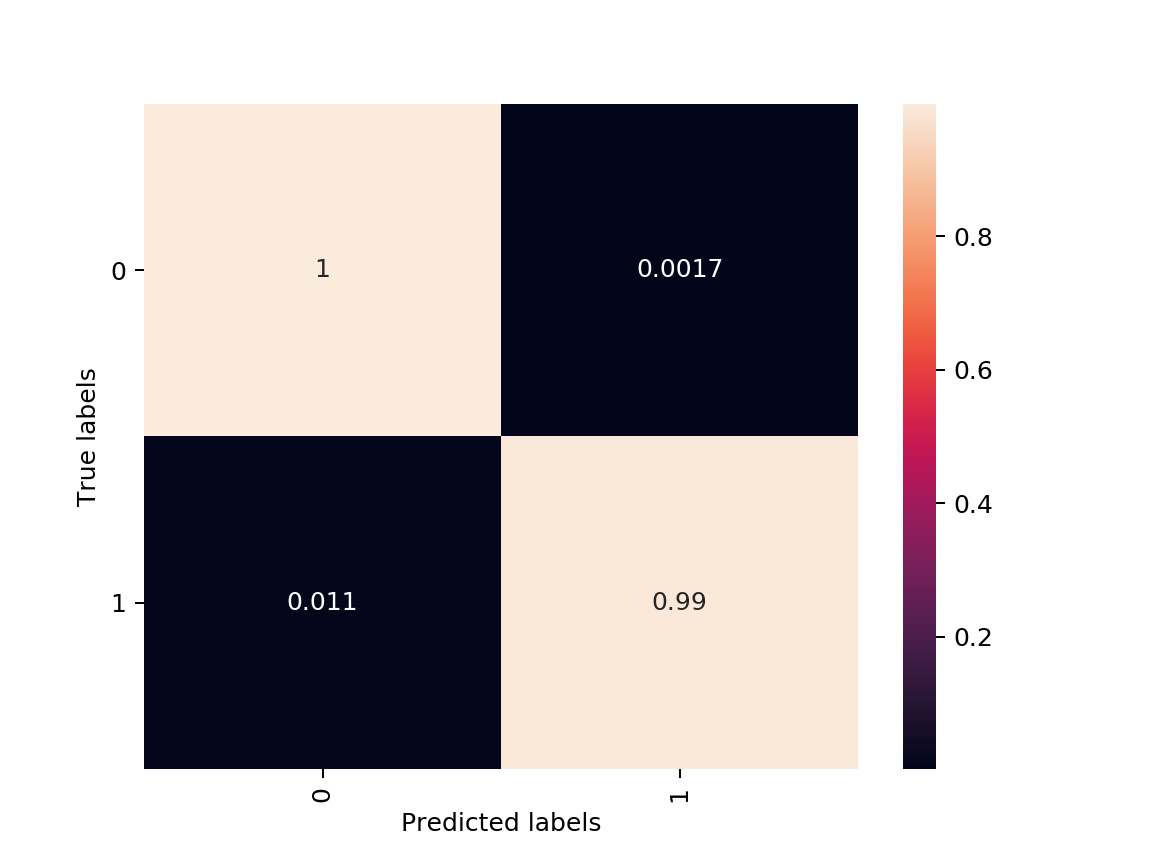
\includegraphics[width =0.45 \linewidth]{figures/egogesture_confusion_matrix}}%
\label{fig:staego}%
\qquad
\subfigure[]{%
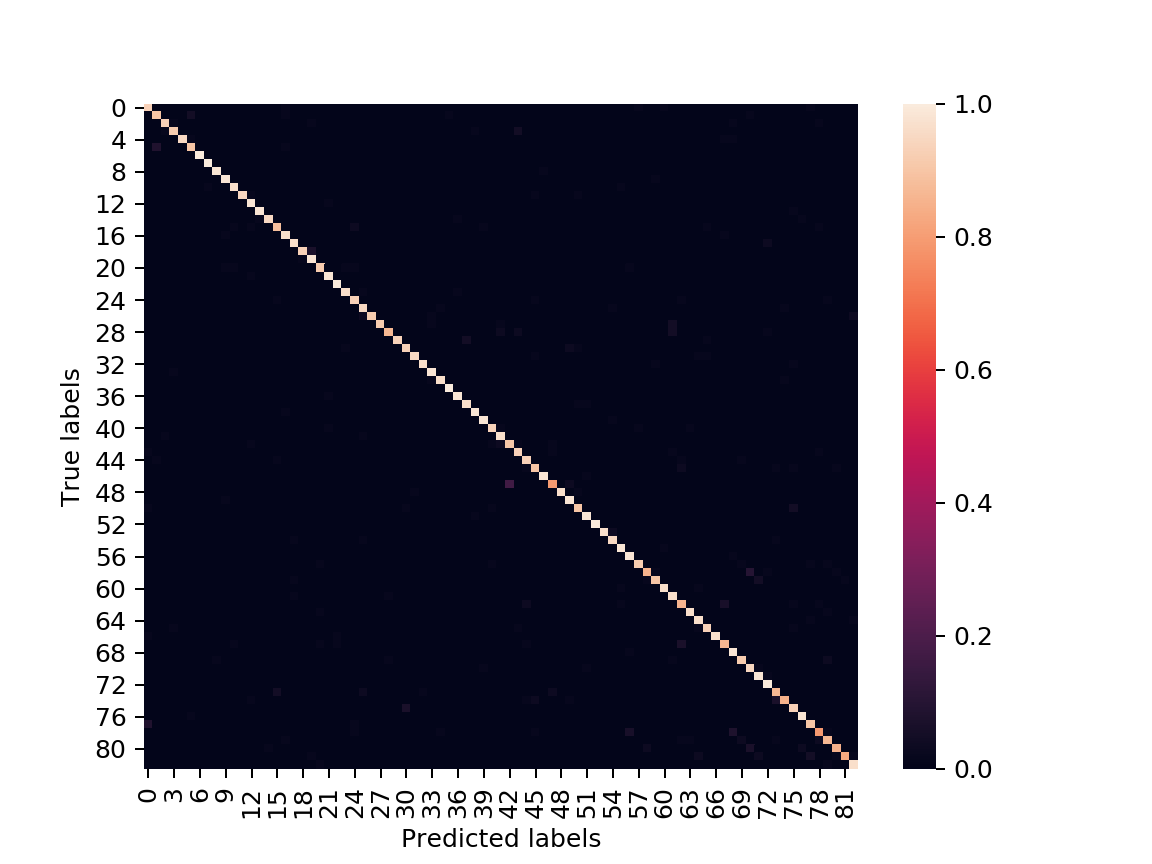
\includegraphics[width = 0.45 \linewidth]{figures/egogesture_confusion_matrix2}}%
\caption{Mormalized confusion matrices for the choosen detector (a) and classifier (b) in \textbf{EgoGesture} dataset.}
\label{fig:egocm}
\end{figure}
\begin{table}[t!]
    \centering
    \begin{tabular}{lcccc}
        \specialrule{.1em}{.5em}{.5em}
        \multicolumn{1}{c}{\multirow{2}{*}{\textbf{Model}}} & \multicolumn{1}{c}{\multirow{2}{*}{\textbf{Input}}} & \multicolumn{3}{c}{\textbf{Modality}}                                   \\ \cline{3-5} \addlinespace
        \multicolumn{1}{c}{}      & \multicolumn{1}{c}{}    & \textbf{RGB} & \textbf{Depth} & \textbf{RGB-D} \\
        \specialrule{.1em}{.3em}{.3em}
        VGG-16 \cite{zhang_egogesture:_2018}          & 16-frames     & 62.50    & 62.30    & 66.50    \\
        VGG-16 + LSTM \cite{zhang_egogesture:_2018}   & 16-frames     & 74.70    & 77.70    & 81.40    \\
        C3D                                           & 16-frames     & 86.88    & 88.45    & 89.45    \\ 
        ResNeXt-101                                   & 16-frames     & 90.94    & 91.80    & 91.82    \\ 
        C3D+LSTM+RSTTM \cite{zhang_egogesture:_2018}  & 16-frames     & 89.30    & 90.60    & 92.20    \\
        \specialrule{.1em}{.3em}{.3em}
        ResNeXt-101     & 32-frames     & 93.75          & \textbf{94.03}           & 93.93             \\ 
        \specialrule{.1em}{.5em}{.5em}
    \end{tabular}
    \caption{Comparison with state-of-the-art on the test set of EgoGesture dataset.}
	\label{tab:nv_benchmark}
\end{table}

Thirdly, the modalities (RGB, Depth and RGB-D) are investigated through fixing window-size of input frames. We can see that the models with RGB-D and Depth modalities always show better performance than the models with RGB. Because Depth sensor filters out background motion, and it allow models to focus more on the hand motion, and learn discriminative features better. Additionally, The state-of-the-art accuracies in classification task of EgoGesture datasets are shown in Table \ref{tab:egogesture_benchmark}. We can clearly say that ResNet-101 architecture with 32-frames of Depth modality outperforms the proposed architecture in \cite{zhang_egogesture:_2018}.  \\

After offline classification results, we decided to use ResNet-10 with window of size 8 and Depth images as our detector even though the ones with 24-frames and 32-frames have higher accuracy rate. This is because having smaller window size allows the detector to be more robust in detection of the start and the end of gestures. Moreover, It is very critical that we do to miss any gestures, and this is highly dependent on the detector's recall rate. The detailed results of this model is shown in Table \ref{tab:egogesture_det}. \\

Finally, we investigated the performance of the detector (ResNet-10 with window size of 8 and trained on Depth images) and the classifier (ResNext-101 with window size of 32 and trained on Depth images) with confusion matrix shown in Figure \ref{fig:egocm}.\\
\clearpage
\section{Offline Results Using nvGesture Dataset}
\begin{table}[h!]
    \centering
    \begin{tabular}{ccccc}
        \specialrule{.1em}{.5em}{.5em}
        \multicolumn{1}{c}{\multirow{2}{*}{\textbf{Model}}} & \multicolumn{1}{c}{\multirow{2}{*}{\textbf{Input}}} & \multicolumn{3}{c}{\textbf{Modality}}                                   \\ \cline{3-5} \addlinespace
        \multicolumn{1}{c}{}                       & \multicolumn{1}{c}{}                       & \multicolumn{1}{c}{\textbf{RGB}} & \multicolumn{1}{c}{\textbf{Dept}h} & \textbf{RGB-D} \\
        \specialrule{.1em}{.3em}{.3em}
        C3D             & 16-frames     & 62.67          & 70.33           & 64.10             \\ 
        C3D             & 24-frames     & 65.35          & 70.33           & 66.40             \\ 
        C3D             & 32-frames     & 73.86          & \textbf{77.18}           & 72.61             \\ 
        \specialrule{.1em}{.3em}{.3em}
        ResNeXt-101     & 16-frames     & 66.40          & 72.82                    & 74.65    \\ 
        ResNeXt-101     & 24-frames     & 72.40          & 79.25          & 75.31             \\ 
        ResNeXt-101     & 32-frames     & 78.63          & \phantom{\textbf{*}}\textbf{83.82}\textbf{*}           & 79.67             \\ 
        \specialrule{.1em}{.5em}{.5em}
    \end{tabular}
    \caption{Classifier's classification results on the test set of \textbf{nvGesture} dataset.}
	\label{tab:nvgesture_classifier}
\end{table}
\begin{table}[h!]
    \centering
    \begin{tabular}{ccccc}
        \specialrule{.1em}{.5em}{.5em}
        \multicolumn{1}{c}{\multirow{2}{*}{\textbf{Model}}} & \multicolumn{1}{c}{\multirow{2}{*}{\textbf{Input}}} & \multicolumn{3}{c}{\textbf{Modality}}                                   \\ \cline{3-5} \addlinespace
        \multicolumn{1}{c}{}                       & \multicolumn{1}{c}{}                       & \multicolumn{1}{c}{\textbf{RGB}} & \multicolumn{1}{c}{\textbf{Dept}h} & \textbf{RGB-D} \\
        \specialrule{.1em}{.3em}{.3em}
        ResNet-10     & 8-frames      & 70.22          &  \phantom{\textbf{}} 97.30\textbf{*}        & 93.15    \\ 
        ResNet-10     & 16-frames     & 85.90          & 97.82           & 94.81    \\ 
        ResNet-10     & 24-frames     & 89.00          & \textbf{98.02}           & 97.30    \\ 
        ResNet-10     & 32-frames     & 93.88         & 97.30            & 95.33    \\ 
        \specialrule{.1em}{.3em}{.3em}
    \end{tabular}
    \caption{Detector's classification results on the test set of \textbf{nvGesture} dataset.}
	\label{tab:nvgesture_detector}
\end{table}
In nvGesture dataset, we followed similar validation procedure to EgoGesture dataset except that nvGesture dataset does not have a validation set so we trained our models for fixed number of epochs (30) and used the last one as our reference.\\ 
\begin{table}[b!]
	\centering
	\begin{tabular}{lccc}
		\specialrule{.1em}{.5em}{.5em}
		\textbf{Modality} & \textbf{Recall} & \textbf{Precision} & \textbf{f1-score}  \\ 
		\specialrule{.1em}{.3em}{.3em}
		RGB            & 70.22	    & 80.31     & 74.93  \\
		Depth          & 97.30		& 97.41		& \textbf{97.35}   \\
		RGB-D          & 93.15		& 93.31		& 93.23 \\
		\specialrule{.1em}{.3em}{.3em}
	\end{tabular}
	\caption{Detection results on the test set of \textbf{nvGesture} dataset.}
	\label{tab:nvgesture_det}
\end{table}

Performance of the detector and the classifier architectures can be seen in Table \ref{tab:nvgesture_detector} and Table \ref{tab:nvgesture_classifier}, respectively. These results confirm our implications in EgoGesture dataset as models with Depth and RGB-D modalities shows better performance than models with RGB. Also In nvGesture dataset, duration of every gesture corresponds to exactly 81 frames. Consequently, the more window-size of model the higher accuracy rate as it is the case in EgoGesture dataset as well. \\

Additionally, Table \ref{tab:nvgesture_classifier} shows comparision betwenn the state-of-the-art models and our classifer architectures. ResNet-101 with 32 frames showed comparable results with R3DCNN \cite{molchanov_online_2016}. Similarly, the confusion matrices for the selected detector and classifier on nvGesture dataset can be seen in Figure \ref{fig:nvcm}.\\
\begin{figure}[h!]%
\centering
\subfigure[]{%
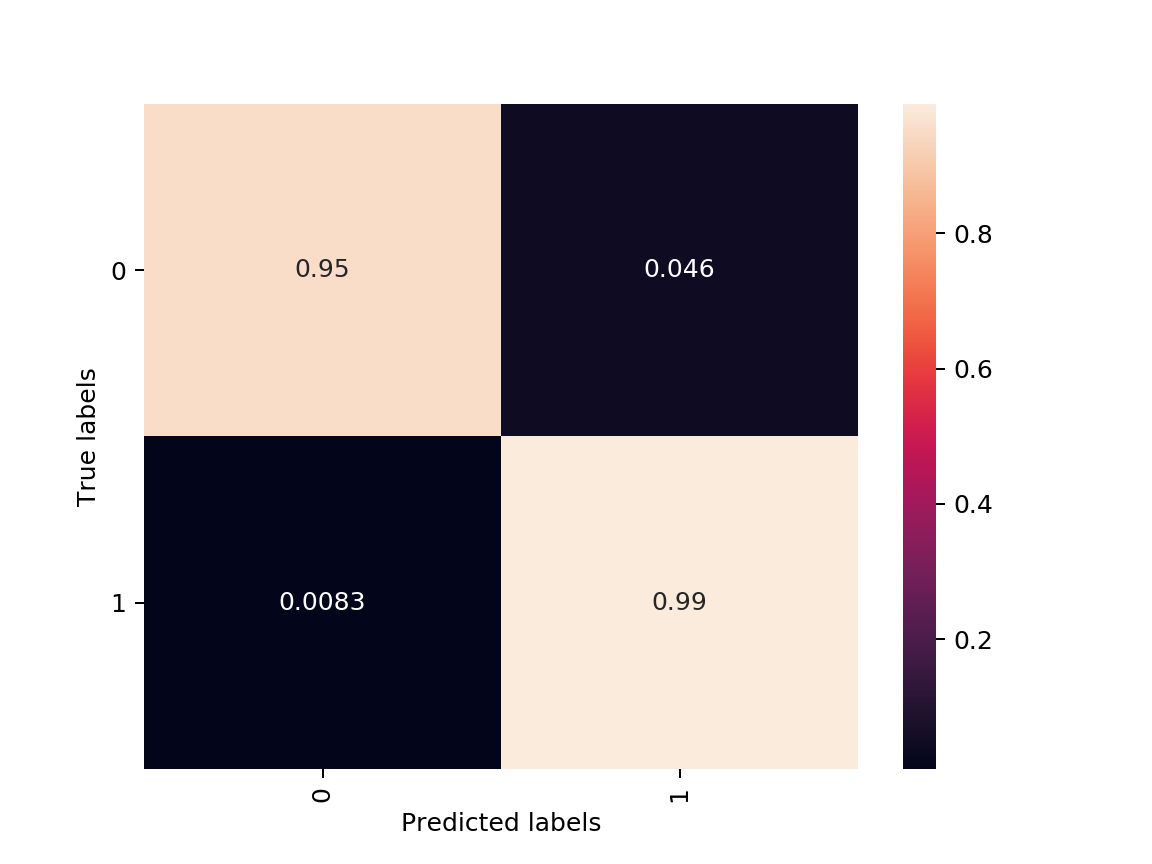
\includegraphics[width =0.45 \linewidth]{figures/nv_confusion_matrix}}%
\label{fig:staego}%
\qquad
\subfigure[]{%
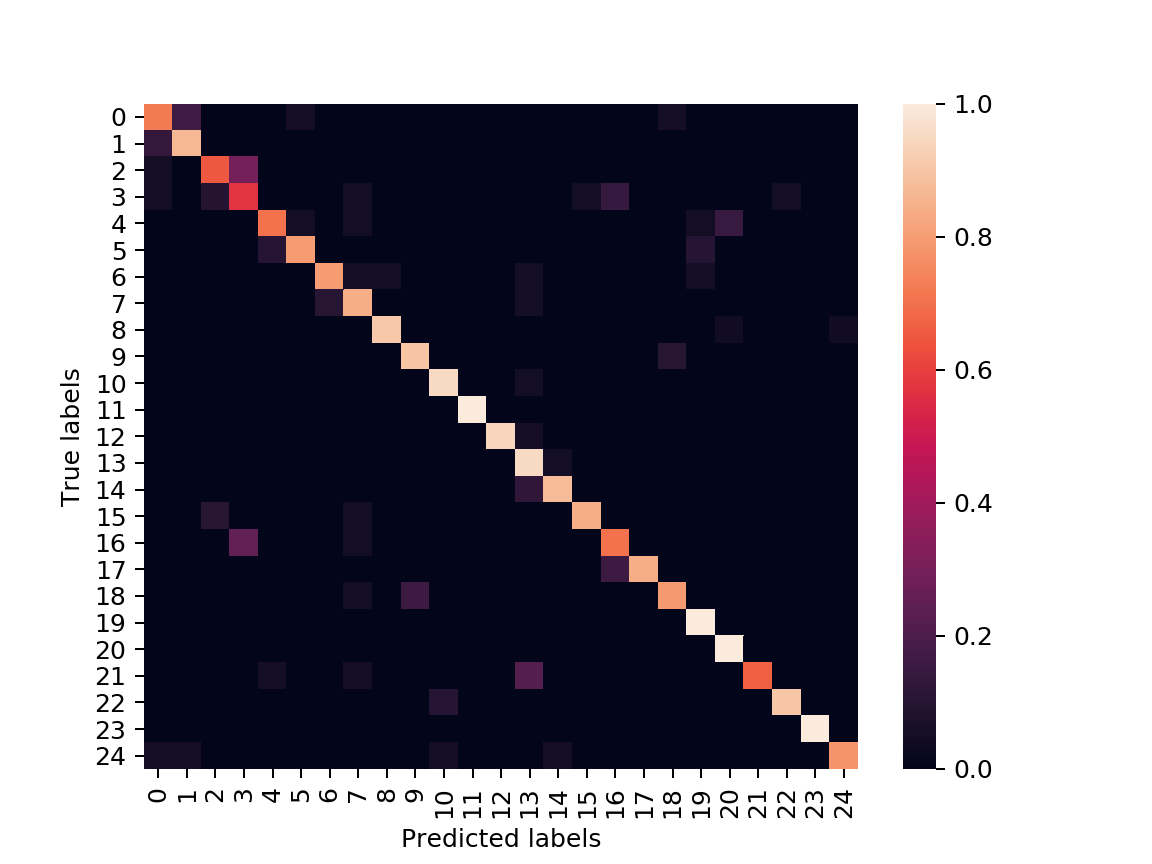
\includegraphics[width = 0.45 \linewidth]{figures/nv_confusion_matrix2}}%
\caption{Normalized confusion matrices for the chosen detector (a) and classifier (b) in \textbf{nvGesture} dataset.}
\label{fig:nvcm}
\end{figure}

\begin{table}[t!]
    \centering
    \begin{tabular}{lccccc}
        \specialrule{.1em}{.5em}{.5em}
        \multicolumn{1}{c}{\multirow{2}{*}{\textbf{Model}}} & \multicolumn{1}{c}{\multirow{2}{*}{\textbf{Input}}} & \multicolumn{4}{c}{\textbf{Modality}}                                   \\ \cline{3-6} \addlinespace
        \multicolumn{1}{c}{}      & \multicolumn{1}{c}{}    & \textbf{RGB} & \textbf{Depth} & \textbf{RGB-D} &   \textbf{RGBD + flow} \\
        \specialrule{.1em}{.3em}{.3em}
        C3D             & 16-frames     & 62.67          & 70.33           & 64.10          & -   \\ 
        R3DCNN \cite{molchanov_online_2016}                          & 16-frames     & 74.10    & 80.30    & -  & 83.8  \\ 
       ResNeXt-101     & 16-frames     & 66.40          & 72.82                    & 74.65   & - \\
        \specialrule{.1em}{.3em}{.3em}
        ResNeXt-101     & 32-frames     & 78.63        & \phantom{\textbf{*}}\textbf{83.82}\textbf{*}           & 79.67        & -       \\ 
        \specialrule{.1em}{.5em}{.5em}
    \end{tabular}
    \caption{Comparison with state-of-the-art on the test set of nvGesture dataset. In \cite{molchanov_online_2016} a proposed architecture with RGB, Depth, optical flow (annotated as "flow" in the Table) modalities achieves state-of-the-art 83.8\% accuracy.}
	\label{tab:egogesture_benchmark}
\end{table}

\clearpage
\section{Real-Time Classification Results}
\begin{figure}[b!]%
\centering
\subfigure[]{%
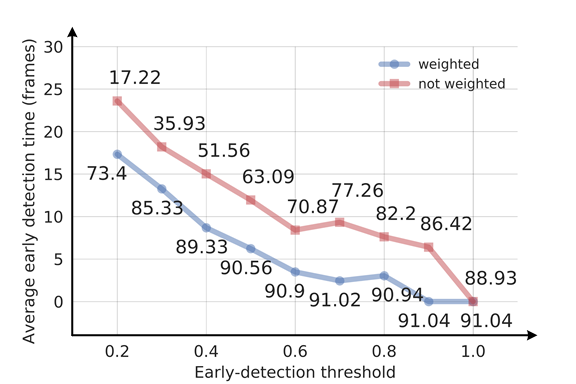
\includegraphics[width =0.6 \linewidth]{figures/egogesture_det}}%
\label{fig:staego}%
\qquad
\subfigure[]{%
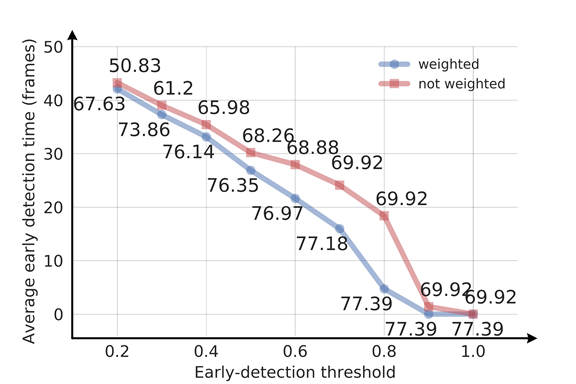
\includegraphics[width = 0.6 \linewidth]{figures/nv_det}}%
\caption{Correctly predicted classes early-detection durations with respect to different thresholds (0.2-1.0) in \textbf{(a) EgoGesture} and  
\textbf{(b) nvGesture} datasets. Numerals on each data point represent the overall Levenshtein accuracies. Blue color refers to the "weighted" approach in single-time activation, and green color refers to "not weigted" approach. In both cases, duration between the end of gesture and detected time decreases as threshold increases, which is expected. Besides that, we can see that the weighted approach increases the Levenshtein accuracies drastically.}
\label{fig:stanv}
\end{figure}
 In online (real-time) evaluation, we selected best performing models in both dataset, which have \textbf{*} sign in corresponding Tables. Egogesture and nvGesture respectively have 431 and 482 video samples in their test set. We evaluated our proposed architecture on each video seperately and calculated an average Levenshtein accuracy at the end. We achieved 91.04\% (in Egogesture ) and 77.39\% (in nvGesture) overall Levenshtein accuracy.\\

Moreover, the early detection times are investigated by simulating different early detection threshold levels ($\tau_{early}$) levels (0.2-1.0). Figure \ref{fig:stanv} compares early detection durations of weigted-averaging and uniformly-averaging approaches for both EgoGesture and nvGesture datasets. As expected, the more the early detection threshold is the later the models detect the gesture. Additionally weighted approach clearly achieves better Levenshtein accuracy rate for the same early-detection threshold levels. This proves that we managed to get rid of the ambiguity at the beginning of gestures by assigning lower weights.\\ 

As a result, it is important to note that, comparison of the Levenshtein metric and offline accuracy is not fair even though there is a strong positive correlation between them. This is because the Levenshtein metric not only evaluate misclassification rate but also multiple prediction rate of the same gesture. Nevertheless, the offline accuracy rate of a model can be also considered as the upper bound for the Levenshtein metric.\\
% Conlusion and outlook
\chapter{Conclusion}
\label{ch:conclusion}

\section{Conclusion}
This thesis presents a novel two-model hierarchical architecture for real-time  hand gesture recognition systems that enable the integration of deep learning models, which performs well offline. We evaluated the proposed architecture on two dynamic hand gesture datasets (EgoGesture and nvGesture), and achieved similar results for both of them.\\ 

After offline classification results, we concluded that Depth modality allow the model learn better than other modalities as it only captures the hand movement and filter out the background motion. Also it is clear that as the number of consecutive frames in a window increased, the model performs better as it is easier for the model to capture temporal pattern of gestures. As the windows-size chosen closer to the mean number of gesture durations (in frames), the model perform better in learning the patter. One negative outcome of using bigger window size is that the floating point operations for one iteration increases linearly.\\

For the evaluation of real-time gesture recognition models, we utilized a new metric approach, the Levenshtein accuracy, that validate single-time activation precision of a model. Our results show that, weighted-averaging of class probability over time improves the overall performance together with allowing early detection of gestures. Fixing the threshold, Levenshtein accuracy of the weighted approach is always more than the not-weighted approach. This proves that the ambiguity at the beginning of gestures, especially dynamic gestures,  can be eliminated by assigning smaller weights. \\

We acquired single-time activation per gesture by using difference between highest two average  class probabilities as a confidence measure. However, as a future work we would like to investigate more on the statistical hypothesis testing for the confidence measure of the single-time activation. Also, we intend to utilize different weighting approaches in order to increase the performance even further.  \\







%%%%%%%%%%%%%%
% Backmatter %
%%%%%%%%%%%%%%
% \cleardoublepage
% \begin{appendix}
% \chapter{Upper Bounds on the Expected Error Probability}
\label{ch:appendix}

\section{Recognition Accuracy Rate}



% \end{appendix}
% \backmatter % Here, because appendix has still the mainmatter formatting

% Writes only, e.g., "bibliography" on top of those sections
\renewcommand{\chaptermark}[1]{\markboth{#1}{}}
\renewcommand{\sectionmark}[1]{\markright{#1}{}}

  
\cleardoublepage
\addcontentsline{toc}{chapter}{References}
\bibliographystyle{alpha} % Bibliography
% Add your works that are not cited in the text with the \nocite* command


\bibliography{bibliography/egbib}

\end{document}
